\ifdefined\pdfminorversion
  \pdfminorversion=7
\fi
\documentclass[12pt]{article}

\usepackage[a4paper,margin=1in]{geometry}
\usepackage[T1]{fontenc}
\usepackage[utf8]{inputenc}
\usepackage{lmodern}
\usepackage{microtype}
\usepackage{amsmath,amssymb,amsthm,mathtools,bm}
\usepackage{booktabs,tabularx,array,multirow}
\usepackage{longtable}
\usepackage{graphicx}
\usepackage{enumitem}
\usepackage[round,authoryear]{natbib}
\usepackage{xcolor}
\usepackage{url}
\usepackage[pagebackref]{hyperref}
\usepackage[nameinlink,noabbrev]{cleveref}
\usepackage[mathlines]{lineno}
\usepackage{setspace}
\usepackage{caption}
\usepackage{float}

% Reusable table columns: fixed-width text and numeric entries are vertically
% centred, while Y lets tabularx allocate the remaining width to prose.
\newcolumntype{L}[1]{>{\raggedright\arraybackslash}m{#1}}
\newcolumntype{C}[1]{>{\centering\arraybackslash}m{#1}}
\newcolumntype{Y}{>{\raggedright\arraybackslash}X}

\hypersetup{
 colorlinks=true,
 linkcolor=blue!45!black,
 citecolor=blue!45!black,
 urlcolor=blue!45!black,
 pdftitle={Anytime-valid weighted survival tests for exact failures and completed assessment windows},
 pdfsubject={Weighted conditional survival comparisons for exact failures and common completed assessment windows},
 pdfkeywords={anytime-valid inference, e-values, right censoring, interval censoring, weighted logrank tests, covariate stratification},
 pdfauthor={Hien Duy Nguyen and Liming Xiang}
}

\renewcommand*{\backref}[1]{}
\renewcommand*{\backrefalt}[4]{%
 \ifcase #1\relax
 \or \space(cited on page~#2)%
 \else \space(cited on pages~#2)%
 \fi}
\renewcommand*{\backrefsep}{, }
\renewcommand*{\backreftwosep}{ and }
\renewcommand*{\backreflastsep}{, and }

\setlist[itemize]{topsep=3pt,itemsep=2pt,parsep=0pt}
\setlist[enumerate]{topsep=3pt,itemsep=2pt,parsep=0pt}
\setlength{\emergencystretch}{2em}
\allowdisplaybreaks
\captionsetup{font=small,labelfont=bf}

\newtheorem{theorem}{Theorem}[section]
\newtheorem{proposition}[theorem]{Proposition}
\newtheorem{corollary}[theorem]{Corollary}
\newtheorem{lemma}[theorem]{Lemma}
\newtheorem{condition}[theorem]{Condition}
\theoremstyle{definition}
\newtheorem{definition}[theorem]{Definition}
\theoremstyle{remark}
\newtheorem{remark}[theorem]{Remark}

\newcommand{\KL}{\mathrm{KL}}

\title{\textbf{Anytime-valid weighted survival tests for exact failures and completed assessment windows}}
\author{%
 Hien Duy Nguyen$^{1,2}$ and Liming Xiang$^3$\\[0.6em]
 \parbox{0.94\textwidth}{\centering\small
 $^1$School of Computing, Engineering and Mathematical Sciences,\\
 La Trobe University, Bundoora, Victoria, Australia\\[0.3em]
 $^2$Institute of Mathematics for Industry,\\
 Kyushu University, Fukuoka, Japan\\[0.3em]
 $^3$School of Physical and Mathematical Sciences,\\
 Nanyang Technological University, Singapore}%
}
\date{}

\begin{document}
\maketitle
\linenumbers

\begin{abstract}
Repeated application of a fixed-analysis weighted logrank test does not retain its nominal type-I error guarantee. Within the conditional likelihood-ratio framework of J.~ter Schure, M.~F.~P\'erez-Ortiz, A.~Ly and P.~D.~Gr\"unwald [\emph{The anytime-valid logrank test: Error control under continuous monitoring with unlimited horizon}, \emph{The New England Journal of Statistics in Data Science} 2(2), 190--214, 2024], we develop weighted comparisons for exact failures with right censoring and first detections within common completed assessment windows. We specify eligibility and information rules and give a sufficient independent-stream model for combining the two observation schemes. The finite-sample guarantee requires conditional exchangeability of event allocation within each comparison stratum. Classical survival weights define exponential alternatives whose accumulated log likelihood ratio has the corresponding weighted Cochran--Mantel--Haenszel or logrank score as its derivative at the null. A fixed-margin calculation relates relative weights to local score shifts. Simulations compare complete specifications of weight, normalization and coefficient, monitoring rules, and observation designs. At $n=500$ with interval observations, normalized Fleming--Harrington processes have higher power than logrank for the studied delayed effect under two calibration regimes: holding normalization and coefficient fixed across alternatives, or using design-specific normalization and a coefficient selected under the true alternative. For the studied early effect, Peto--Peto has lower power than logrank under the fixed choices and higher power under the alternative-specific choices. These comparisons condition on the realized independent pilot calibrations. For the e-process specifications studied here, monitoring flexibility can entail substantial power loss at small sample sizes. Retrospective clinical reconstructions illustrate the additional assumptions and information loss introduced by grouping irregular visits.

\end{abstract}

\noindent\textbf{Keywords:} e-values; right censoring; interval censoring; sequential monitoring; weighted logrank tests; covariate stratification.

\section{Introduction}
\label{sec:introduction}

Survival comparisons involve two design choices: which differences over follow-up matter, and when the evidence will be examined. The classical logrank test is effective under approximately proportional hazards \citep{Mantel1966,Cox1972}. Weighted tests give more emphasis to particular stages of follow-up: Gehan--Breslow weights emphasize earlier failures \citep{Gehan1965}, Fleming--Harrington weights can target early or delayed differences \citep{HarringtonFleming1982}, and Gray--Tsiatis weighting is motivated by long-term survival differences \citep{GrayTsiatis1989}. Repeatedly applying a fixed-analysis test and stopping at significance can inflate the false-positive probability. Group-sequential boundaries and alpha-spending methods address planned monitoring \citep{OBrienFleming1979,LanDeMets1983,Slud1984}. An anytime-valid test instead controls the probability of ever crossing its rejection threshold, including under an unplanned extension of follow-up.

The observation scheme determines which comparisons support that guarantee. Exact failures with right censoring lead to risk-set comparisons \citep{AndersenEtAl1993}. Interval assessments, such as angiography for cardiac allograft vasculopathy, locate the event between a last negative and a first positive visit \citep{SharplesEtAl2003}. Imputing an exact failure time changes the ordering used by a rank test \citep{LawBrookmeyer1992}. Existing interval-censoring methods use the intervals directly for survival estimation \citep{Turnbull1976}, regression \citep{Finkelstein1986}, and group comparison \citep{Sun1996,FayShaw2010}; see \citet{Sun2006}. These fixed-analysis methods do not by themselves justify unrestricted repeated testing. Here we study first detections in common completed assessment windows, rather than arbitrary individual interval-censoring schedules.

The validity mechanism is inherited from \citet{TerSchureEtAl2024}. Their equation~(3.5) permits past-dependent numerator distributions. For grouped assessments, their Section~3.3 uses the same hypergeometric conditional null as in this work. A normalized working alternative divided by that null gives a factor with conditional mean one; multiplying the factors yields a test martingale. Stratified count-table e-values are also developed by \citet{TurnerGrunwald2023}; survival data additionally require attention to changing risk sets, absorbing failures and incomplete observation.

Our contribution has three parts. First, we specify completed-window eligibility and information rules and give a joint sufficient model for combining exact and grouped observations. Second, we use classical survival weights to define exponential alternatives, identify their score connection and derive a restricted local relative-weight criterion. Third, we compare complete specifications, monitoring rules and observation designs, and examine what is lost when irregular clinical visits are grouped. The conditional normalization argument supplies the validity mechanism for these choices.

At comparison $j$, we use classical survival weights to specify a working alternative for the possible treatment event count $y$ of the form
\[
 q_{\eta,j}^{(w)}(y)\ \propto\ p_{0j}(y)\exp(\eta w_jy),
\]
where $p_{0j}$ is the conditional null mass, $w_j$ is a weight and $\eta$ determines the direction and magnitude of the tilt. The choices cannot use the current group allocation of events. We identify the weighted Cochran--Mantel--Haenszel (CMH) or logrank score as the derivative of the accumulated log process at zero \citep{Cochran1954,MantelHaenszel1959}. This identity explains how classical weights enter the e-process, but does not equate its rejection rule with the classical test. We also derive a relative-weight criterion for a fixed-margin local score shift and distinguish it from log-growth and boundary-crossing objectives.

The use of a weight to specify a time-varying treatment effect has a close antecedent in \citet{LinLeon2017}. They place a chosen time-varying weight in the treatment effect of a Cox model, whose score is the corresponding weighted logrank score. Our exact single-failure tilt has this conditional form when the weight is predictable. The completed-window parameter instead describes conditional event-allocation odds, and repeated-monitoring validity comes from normalization under the stated conditional null law.

For completed windows, we retain only subjects observed through the end of a window, unlike the convention that events precede censoring in \citet[Section~3.3]{TerSchureEtAl2024}. A sufficient model for exact comparisons has common null event intensities within each stratum; for completed windows, conditional exchangeability of the interval event indicators gives the required allocation law. Randomization or a chosen stratification alone is insufficient. Corollary~\ref{cor:mixed-streams} gives a joint model under which these laws hold given the merged history. Such a joint argument is needed because validity in separate filtrations does not automatically transfer to a combined filtration \citep{ChoeRamdas2026}. A study with mixed observation schemes, as in \citet{ZhaoEtAl2008}, can then retain both kinds of records without imputing event times. Keeping exact timing and retaining large comparison sets are competing considerations for power.

Planned monitoring under nonproportional hazards also has a substantial literature. \citet{BrummelGillen2014} use constrained boundaries to monitor weighted logrank statistics with nonlinear information growth while preserving a planned group-sequential design's operating characteristics. \citet{KunduSarkar2021} study information fractions for Fleming--Harrington tests, \citet{WangLuoZheng2021} develop group-sequential max-combo designs, and \citet{BoherEtAl2024} study group-sequential supremum logrank statistics. Adaptive weight selection is considered by \citet{LiWang2026}. These works address related choices of effect pattern, weighting and monitoring; the present construction uses conditional likelihood ratios to permit monitoring or continuation without a fixed number of analyses. Our simulation comparison with the O'Brien--Fleming-type boundary OBF(1.96) is an illustrative conservative reference, rather than an efficiency comparison with calibrated group-sequential designs.

Section~\ref{sec:methods} starts with a single-failure calculation and states the observation assumptions. Section~\ref{sec:theory} separates validity, the score identity and the restricted local weighting criterion. The simulations in Section~\ref{sec:simulation} lead with specifications held fixed across alternatives, then examine how alternative-specific coefficient selection changes the conclusions. Section~\ref{sec:clinical} treats the clinical analyses as exploratory calculations under working observation models. Proofs, full numerical grids and additional diagnostics are in the appendices.

\section{Proposed method}
\label{sec:methods}

We partition subjects into strata for comparison. Each stratum groups subjects with the same prespecified prognostic categories and compatible observation schemes and time scales.

Consider one exact failure in a stratum containing $N_{1j}$ treatment subjects and $N_{0j}$ controls at risk, with no simultaneous failures within the stratum. Under a common null event intensity, each subject is equally likely to be the one who fails. The probability of a treatment failure is therefore $\pi_j=N_{1j}/N_j$, where $N_j=N_{0j}+N_{1j}$. Let $Y_j$ indicate a treatment failure. Before using its group identity, choose a positive conditional-odds alternative $\theta_j$. Its likelihood ratio against the null is
\begin{equation}
 e_j=\frac{\theta_j^{Y_j}}{1-\pi_j+\pi_j\theta_j},
 \qquad \theta_j=\exp(\eta w_j).
 \label{eq:single-failure-factor}
\end{equation}
Here $w_j$ is a survival weight and $\eta$ sets the strength and direction of the alternative. With equal risk-set sizes and $\theta_j=1/2$, a control failure multiplies the evidence by $4/3$, whereas a treatment failure multiplies it by $2/3$. Under the null, their average is one. Multiplying such factors accumulates evidence that can increase or decrease after each failure. For a completed interval containing several newly detected events, the same argument uses a hypergeometric distribution instead of a Bernoulli distribution.

\subsection{The null hypothesis and comparison tables}
\label{sec:probability-setup}
\label{sec:covariate-adjustment}

The null concerns event allocation within each comparison, conditional on the observed history and recorded prognostic covariates. For exact failures, a sufficient model gives subjects in the current stratum a common event intensity. For grouped assessments, the newly detected event indicators must be conditionally exchangeable within a common completed window. Marginal equality of the two survival distributions alone does not establish these conditions. Event risks may differ between strata, but randomization or a prespecified stratification alone does not remove risk differences within a stratum.

For subject $i$, let $G_i\in\{0,1\}$ denote control or treatment, $X_i$ the baseline covariates, and $T_i,C_i$ the event and censoring times. We allow $T_i=\infty$. A fixed map $\mathsf s(X_i)\in\{1,\ldots,K_X\}$ assigns prognostic strata before follow-up and is applied identically to both groups. Subjects with incompatible observation schemes or time scales are also separated into monitoring strata. The unstratified analysis has $K_X=1$. Formal probability-space and observation-record conventions are collected in Appendix~\ref{app:formal-setup}.

At an exact failure, use the risk set immediately before that failure in its monitoring and prognostic stratum. At an interval assessment, use subjects known event-free at $\ell_j$ and observed through $r_j$ for a common completed interval $(\ell_j,r_j]$, where $0\leq\ell_j<r_j<\infty$. First detections at $r_j$ are its events. This includes left-censored first detections when $\ell_j=0$. Exclude intervals not completed at the common endpoint $r_j$. Inclusion based on terminal event status obtained through another ascertainment mechanism requires a separate justification of Condition~\ref{ass:allocation} for the retained comparison. Each retained event enters once, when its occurrence first becomes known.

Index these comparisons chronologically by $j$. Let $\mathsf R_j^{\mathrm{obs}}$ be the eligible set before restricting to prognostic stratum $k_j$. Write $\mathsf R_j$ for the restricted set. The event set $\mathsf A_j$ contains the newly observed events in this stratified set $\mathsf R_j$, so that
\[
 \mathsf R_j=\{i\in\mathsf R_j^{\mathrm{obs}}:\mathsf s(X_i)=k_j\},
 \qquad \mathsf A_j\subseteq\mathsf R_j,
\]
and the group sizes and event counts are
\begin{equation}
 \begin{aligned}
 N_{gj}&=\sum_{i\in\mathsf R_j}\mathbf 1\{G_i=g\},\quad g\in\{0,1\},
 \qquad N_j=N_{0j}+N_{1j},\\
 M_j&=|\mathsf A_j|,\qquad Y_j=\sum_{i\in\mathsf A_j}G_i.
 \end{aligned}
 \label{eq:update-counts}
\end{equation}
The sets and counts depend on the observed history and fixed stratification. Empty comparison sets are omitted. Every update has the following table:
\begin{center}
\begin{tabular}{lccc}
\toprule
 & Newly observed event & No newly observed event & Total\\
\midrule
Treatment & $Y_j$ & $N_{1j}-Y_j$ & $N_{1j}$\\
Control & $M_j-Y_j$ & $N_{0j}-M_j+Y_j$ & $N_{0j}$\\
\midrule
Total & $M_j$ & $N_j-M_j$ & $N_j$\\
\bottomrule
\end{tabular}
\end{center}
An exact failure has $M_j=1$; a completed assessment window may have several events. A window with no events has factor one, but its negative assessments establish eligibility for later comparisons. Other zero-variance tables also have factor one; their recorded observations can still update later comparison sets within the permitted history.

\subsection{Information and the conditional null distribution}
\label{sec:information-flow}

Weights and alternatives may use past observations, the current comparison set and its total event count, but not the current allocation of those events between groups. Let $\mathfrak F_0$ contain group labels, recorded covariates, the fixed stratification and design information. The filtration $\mathfrak F_j$ contains all observations incorporated through update $j$. If $O_j$ records the observation scheme, failure time or interval, and monitoring and prognostic strata, define
\begin{equation}
 \mathfrak K_j=\mathfrak F_{j-1}\vee\sigma(O_j,\mathsf R_j),
 \qquad
 \mathfrak G_j=\mathfrak K_j\vee\sigma(M_j).
 \label{eq:intermediate-sigma-algebra}
\end{equation}
Thus $\mathfrak G_j$ adds the margins without adding the event identities. We require
\[
 \mathfrak F_{j-1}\subseteq\mathfrak K_j\subseteq\mathfrak G_j\subseteq\mathfrak F_j,
 \qquad \mathfrak G_j\vee\sigma(\mathsf A_j)\subseteq\mathfrak F_j.
\]
Entry, censoring and assessment information arriving between updates is incorporated before the next comparison. Simultaneous updates in disjoint strata use a prespecified order, excluding unprocessed event allocations until their turn. The conditional allocation null below must hold given earlier observations from every stratum, including allocations already processed at the same time. A prespecified order alone does not establish that null. This specifies the information an analysis may use; it does not require physical release of data in separate stages.

Write $\mathcal P_0$ for the family of laws satisfying the following conditional null, and $\mathbb P_0,\mathbb E_0$ for probability and expectation under any such law. Conditional statements hold almost surely.
\begin{condition}[Conditional allocation null]
\label{ass:allocation}
For every $\mathbb P_0\in\mathcal P_0$, conditional on $\mathfrak G_j$, each subset of $\mathsf R_j$ containing $M_j$ subjects has the same probability of being the event set $\mathsf A_j$, $\mathbb P_0$-almost surely.
\end{condition}
Consequently, $Y_j\mid\mathfrak G_j\sim\mathrm{Hypergeom}(N_j,N_{1j},M_j)$, with support
\[
 \mathcal Y_j=\{\max(0,M_j-N_{0j}),\ldots,\min(M_j,N_{1j})\}
\]
and mass function
\begin{equation}
 p_{0j}(y)=\frac{\binom{N_{1j}}{y}\binom{N_{0j}}{M_j-y}}{\binom{N_j}{M_j}},
 \qquad y\in\mathcal Y_j.
 \label{eq:null-pmf}
\end{equation}
This is the conditional comparison underlying the CMH score. In a completed-window model with independent event indicators and common probability $p_j$, conditioning on $M_j$ cancels $p_j^{M_j}(1-p_j)^{N_j-M_j}$. The unknown event probability may therefore differ between strata and windows without being estimated.

\subsection{Observation assumptions}
\label{sec:observation-mechanisms}

For exact failures, suppose there are no simultaneous failures within a stratum and that censoring and entry preserve the risk-set construction. Under a common null event intensity within the current monitoring and prognostic stratum, the identity of the failing subject is uniform over the current risk set, conditional on the continuous-time history immediately before the failure and on its time \citep{AndersenEtAl1993,FlemingHarrington1991}.

This implies Condition~\ref{ass:allocation} when $\mathfrak G_j$ contains no information beyond that history and failure time. The argument following Proposition~\ref{prop:exact-mark} transfers the result to the update filtration. If an earlier update at the same time has revealed another allocation, the uniform law must also hold conditional on that additional information.

Tied failures can instead be one grouped update only if, given $\mathfrak G_j$, all event subsets of the observed size are equally likely under the null. An event--censoring tie counts as an observed event; censoring without an event removes the subject from subsequent risk sets.

For a completed interval, let $D_{ij}=\mathbf 1\{\ell_j<T_i\leq r_j\}$ for $i\in\mathsf R_j$. Conditional exchangeability of $(D_{ij}:i\in\mathsf R_j)$ given $\mathfrak K_j$ is sufficient. Conditional independence with a common $\mathfrak K_j$-measurable interval event probability is a stronger sufficient condition:
\begin{equation}
 \mathbb P_0(D_{ij}=1\mid\mathfrak K_j)=p_j,
 \qquad i\in\mathsf R_j.
 \label{eq:common-panel-prob}
\end{equation}
Here $p_j$ is an interval event probability, not the treatment risk-set fraction $\pi_j$ in \eqref{eq:single-failure-factor}. Independent censoring preserves this model under the conditions in Proposition~\ref{prop:right-censor}. Merely rounding different visit intervals to the same endpoints does not establish exchangeability.

For a completed-window example, suppose three treatment subjects and two controls are known event-free at $\ell_j$. Given the preselection information $\mathfrak L_j$ of Proposition~\ref{prop:right-censor}, assume independent subject pairs $(D_{ij},B_{ij})$, a common event probability $0<p_j<1$, and independence of event and completion within each pair. Here $B_{ij}$ indicates whether subject $i$ is observed through $r_j$. Consider a completion pattern of positive probability in which one treatment subject is not observed through $r_j$. The retained set has $N_{1j}=N_{0j}=2$. If both controls and neither treatment subject have events, $M_j=2$ and $Y_j=0$. The conditional null probabilities for $Y_j=0,1,2$ are $(1,4,1)/6$. With $\exp(\eta w_j)=1/2$ chosen before using the allocation, the normalizer in \eqref{eq:weighted-factor} is $13/24$, so this table contributes $24/13$. The two retained event-free subjects can enter a later completed window. The incomplete record contributes no event or nonevent to this table; separately ascertained events require the additional justification described in Section~\ref{sec:probability-setup}.

Stratification must make the common-risk model credible. Coarse strata can retain prognostic heterogeneity; fine strata can leave few informative treatment--control comparisons. The construction does not supply unrestricted adjustment for continuous covariates or unmeasured confounding. Attendance or loss to follow-up related to event risk requires an observation model or sensitivity analysis. Existing inverse-probability adjustments cannot simply be inserted without a new conditional e-value argument \citep{HeitjanRubin1991,GillVanDerLaanRobins1997,RobinsFinkelstein2000}.

\subsection{Evidence updates}

Choose any $\mathfrak G_j$-measurable probability kernel $q_j$ supported on $\mathcal Y_j$, with $\sum_{y\in\mathcal Y_j}q_j(y)=1$. Define
\begin{equation}
 e_j=\frac{q_j(Y_j)}{p_{0j}(Y_j)},
 \qquad E_J=\prod_{j=1}^J e_j,\qquad E_0=1.
 \label{eq:generic-eprocess}
\end{equation}
Normalization gives $\mathbb E_0(e_j\mid\mathfrak G_j)=1$. Iterated expectation then makes $E_J$ a nonnegative null martingale. Its value at a fixed update, or at an almost surely finite stopping time, is an e-value: its null expectation is at most one \citep{VovkWang2021,RamdasWang2025}. Theorem~\ref{thm:master} gives the corresponding guarantee for repeated monitoring. No assumption that $q_j$ is the true alternative distribution is needed for validity. If the margins determine $Y_j$, the factor is one; after the final available update, all further factors are also set to one.

We encode a classical survival weight through an exponential tilt. For a finite $\mathfrak G_j$-measurable $w_j$ and finite prespecified $\eta$, set
\begin{equation}
 q_{\eta,j}^{(w)}(y)=
 \frac{p_{0j}(y)\exp(\eta w_jy)}
 {\displaystyle\sum_{u\in\mathcal Y_j}p_{0j}(u)\exp(\eta w_ju)},
 \qquad y\in\mathcal Y_j.
 \label{eq:tilted-pmf}
\end{equation}
This is Fisher's noncentral hypergeometric law with conditional-odds parameter $\exp(\eta w_j)$ \citep{Fog2008}. Its factor and cumulative process are
\begin{equation}
 e_j^{(w)}(\eta)=
 \frac{\exp(\eta w_jY_j)}
 {\displaystyle\sum_{u\in\mathcal Y_j}p_{0j}(u)\exp(\eta w_ju)},
 \label{eq:weighted-factor}
\end{equation}
\begin{equation}
 E_J^{(w)}(\eta)=\prod_{j=1}^J e_j^{(w)}(\eta).
 \label{eq:expanded-eprocess}
\end{equation}
For nonnegative weights, $\eta<0$ targets fewer treatment events than expected under the conditional null. This coefficient is a working conditional log-odds parameter, not generally a population log hazard ratio. The exponential tilt is a particular admissible numerator within the construction based on conditional likelihood ratios of \citet{TerSchureEtAl2024}.

\subsection{Weights and alternative coefficients}
\label{sec:weights}
\label{sec:coefficient-choice}

The weight changes the relative emphasis over follow-up. Table~\ref{tab:weight-guide} gives the choices considered here. For weights based on survival, $\widehat S_{j-1}$ is the current stratum's pooled estimate before using the current event allocation. On a common consecutive assessment grid, initialize $\widehat S_{k,0}=1$ and update stratum $k_j$ by
\begin{equation}
 \widehat S_{k_j,j}=\widehat S_{k_j,j-1}\left(1-\frac{M_j}{N_j}\right),
 \label{eq:pooled-product-limit}
\end{equation}
leaving the other strata unchanged. This is the Kaplan--Meier update for exact failures and its grouped analogue for common assessment windows. Comparisons released together use the estimates available before that release; subsequent pooling must be prespecified. Section~\ref{sec:application-plan} gives the pooling rule used in the clinical examples. Other estimators are admissible if the resulting weights are finite and $\mathfrak G_j$-measurable. The lower bound $s_{\min}>0$ prevents an unbounded inverse weight when estimated survival is small.

\begin{table}[tbp]
\centering
\small
\caption{Classical weights and their intended time emphasis. These choices specify working alternatives; their performance also depends on the coefficient and scale.}
\label{tab:weight-guide}
\begin{tabularx}{\textwidth}{>{\raggedright\arraybackslash}p{0.23\textwidth}>{\raggedright\arraybackslash}p{0.29\textwidth}>{\raggedright\arraybackslash}X}
\toprule
Procedure & Weight $w_j$ & Intended emphasis\\
\midrule
Logrank/CMH (LR) & $1$ & Approximately proportional event intensities\\
Gehan--Breslow (GB) & proportional to $N_j$ & Earlier events, when risk sets are larger\\
Peto--Peto (PP) & $\widehat S_{j-1}$ & Earlier and middle follow-up\\
Fleming--Harrington (FH) & $\widehat S_{j-1}^{\,\rho}(1-\widehat S_{j-1})^{\gamma}$ & Early effects for $\rho>0$, $\gamma=0$; delayed effects for $\rho=0$, $\gamma>0$\\
Gray--Tsiatis (GT) & $1/\max(\widehat S_{j-1},s_{\min})$ & Greater relative emphasis on later differences\\
\bottomrule
\end{tabularx}
\end{table}
Fleming--Harrington parameters satisfy $\rho,\gamma\geq0$, with $0^0=1$. With the same preceding survival estimate in \eqref{eq:pooled-product-limit}, PP denotes this family at $(\rho,\gamma)=(1,0)$ \citep{HarringtonFleming1982}; the simulation column FH uses $(0,1)$. The GT entry is the pooled-survival rule; Appendix~\ref{sec:app-monitoring-comparison} specifies the design-informed variant used in some simulations. The logrank and Gray--Tsiatis motivations are examined in Section~\ref{sec:theory}, including the difference between right-endpoint and preceding-survival weights for finite intervals.

The coefficient and weight scale must be chosen together: multiplying every weight by $a>0$ and dividing $\eta$ by $a$ leaves \eqref{eq:tilted-pmf} unchanged. External estimates or independent design simulations can guide their choice. Such simulations should match the planned observation schedule, censoring and prognostic strata. Mean terminal log evidence, crossing probability by the planned end of follow-up and expected monitoring duration are different objectives. To estimate the last quantity, average first-crossing times across all datasets, assigning the full planned duration to every dataset that does not cross. The median among rejecting datasets alone does not measure expected duration.

When the effect is uncertain, a prespecified mixture can combine complete processes. For example, logrank and Gray--Tsiatis processes may be combined as
\[
 E_J^{\mathrm{mix}}=\lambda E_J^{(1)}+(1-\lambda)E_J^{(2)},
 \qquad 0\leq\lambda\leq1.
\]
A fixed convex combination of null martingales is again a null martingale. The same argument applies to a fixed mixture over coefficients. A finite coefficient $\eta_j$ learned during follow-up may instead use completed earlier updates, so that it is $\mathfrak F_{j-1}$-measurable. Maximizing the already accumulated process over weights or coefficients does not have this justification.

\subsection{Practical analysis procedure}
\label{sec:practical-procedure}

\begin{enumerate}[label=\textbf{Step \arabic*.},leftmargin=2.4cm]
\item State the event comparison and choose prognostic and monitoring strata with compatible risk-time scales. Specify the analysis clock, such as calendar time, time since randomization or attained age, and when each comparison becomes available. Prospective staggered entry must respect availability; retrospective alignment by time since entry need not do so.
\item State the common-risk and observation assumptions supporting Condition~\ref{ass:allocation}. Propositions~\ref{prop:exact-mark} and~\ref{prop:right-censor} give stream-specific models; Corollary~\ref{cor:mixed-streams} gives one joint model. Specify the order of simultaneous comparisons and justify the allocation law given all permitted earlier observations and current margins.
\item Prespecify the direction, weight scale and coefficient or fixed mixture using external or design information. When the effect is uncertain, assess a prespecified mixture or an updating rule based only on past data across plausible alternatives; the simulations do not identify a uniformly preferred choice.
\item At each exact failure or completed interval, form the eligible within-stratum comparison and its margins. Use \eqref{eq:null-pmf} for the null law, with each first event counted once.
\item Evaluate the factor using a weight and alternative that are $\mathfrak G_j$-measurable. Multiply factors in the specified time order, incorporating all comparisons released at a monitoring time before inspecting the process. For a mixture, average the complete component processes with the fixed mixing probabilities.
\item Reject on the first monitored crossing of $1/\alpha$, or 20 when $\alpha=0.05$. Report the evidence path, first crossing, maximum and final value with the comparison and weighting specifications.
\end{enumerate}
Evidence may decline after a valid crossing without reversing the decision. Monitoring regimes may change only according to a prespecified rule or completed earlier observations, preserving the conditional null and avoiding repeated use of an event or overlapping follow-up segment.

\section{Validity, score connection and local weight choice}
\label{sec:theory}

The first result establishes validity by conditional normalization for any admissible numerator. The exponential family then gives the weighted-score identity. A separate fixed-margin calculation asks which relative weights maximize a local score shift; optimizing a survival study's stopping rule is a different problem. Proofs and observation-specific sufficient conditions are in Appendix~\ref{app:proofs}.

\begin{theorem}[Validity by conditional normalization]
\label{thm:master}
Suppose Condition~\ref{ass:allocation} holds at every observation update and $q_j$ is a $\mathfrak G_j$-measurable probability kernel supported on $\mathcal Y_j$. Then $(E_J,\mathfrak F_J)_{J\geq0}$, with $E_J$ defined in \eqref{eq:generic-eprocess} and held constant after the final update, is a nonnegative martingale with $E_0=1$ under every $\mathbb P_0\in\mathcal P_0$. Consequently, for every $\alpha\in(0,1)$,
\begin{equation}
 \mathbb P_0\left(\sup_{J\geq0}E_J\geq\alpha^{-1}\right)\leq\alpha.
 \label{eq:ville-bound}
\end{equation}
\end{theorem}
Ville's inequality \citep{Ville1939} permits monitoring after every valid update without fixing their number in advance. Confidence sequences for the conditional-odds coefficient require the stronger assumption that its model family contains the true conditional laws; see Appendix~\ref{app:confidence-sequences}.

The hypergeometric conditional mean and variance are
\[
 \mu_j=M_j\frac{N_{1j}}{N_j},\qquad
 v_j=\begin{cases}
 M_j\dfrac{N_{1j}}{N_j}\left(1-\dfrac{N_{1j}}{N_j}\right)
 \dfrac{N_j-M_j}{N_j-1},&N_j>1,\\[6pt]
 0,&N_j\leq1.
 \end{cases}
\]
\begin{theorem}[Score and curvature at the null]
\label{thm:score}
Assume that each $w_j$ is finite, $\mathfrak G_j$-measurable and does not depend on $\eta$. For the exponentially weighted process in \eqref{eq:expanded-eprocess},
\begin{equation}
 \left.\frac{\partial}{\partial\eta}\log E_J^{(w)}(\eta)\right|_{\eta=0}
 =\sum_{j=1}^J w_j(Y_j-\mu_j),
 \label{eq:score-identity}
\end{equation}
and
\begin{equation}
 -\left.\frac{\partial^2}{\partial\eta^2}\log E_J^{(w)}(\eta)\right|_{\eta=0}
 =\sum_{j=1}^J w_j^2v_j.
 \label{eq:curvature-identity}
\end{equation}
\end{theorem}
Write $U_J$ and $V_J$ for the right-hand sides of \eqref{eq:score-identity} and \eqref{eq:curvature-identity}, respectively. For a fixed finite sequence of updates and weights independent of $\eta$, the finite-support cumulant functions give the pathwise expansion
\begin{equation}
 \log E_J^{(w)}(\eta)=\eta U_J-\frac{\eta^2}{2}V_J+o(\eta^2),
 \qquad \eta\to0.
 \label{eq:fixed-sequence-log-expansion}
\end{equation}
The linear term is the weighted CMH or logrank score; the quadratic term penalizes the magnitude of the working alternative. This derivative identity does not make the finite-coefficient e-test equivalent to the classical score test or give it the same rejection region. If the score increments are square-integrable, $\mathrm{Var}_0(U_J)=\mathbb E_0(V_J)$. With deterministic counts and weights, this reduces to $\mathrm{Var}_0(U_J)=V_J$.

For the local calculation, fix the finite margin sequence $(N_{0j},N_{1j},M_j)_{j=1}^J$ in advance and treat it as deterministic. Let $Y_j$ be adapted to $(\mathfrak H_j)_{j=0}^J$, with
\[
 \mathbb E_0(Y_j\mid\mathfrak H_{j-1})=\mu_j,
 \qquad \mathrm{Var}_0(Y_j\mid\mathfrak H_{j-1})=v_j.
\]
Under local laws $(\mathbb P_\varepsilon)_{\varepsilon\geq0}$ with null law $\mathbb P_0$, suppose deterministic coefficients $c_j$ satisfy
\begin{equation}
 \mathbb E_\varepsilon(Y_j)=\mu_j+\varepsilon c_jv_j+r_j(\varepsilon),
 \qquad r_j(\varepsilon)=o(\varepsilon),
 \label{eq:main-local-shift}
\end{equation}
for each $j$ as $\varepsilon\downarrow0$.

\begin{theorem}[Relative weights maximizing a fixed-margin local score shift]
\label{thm:optimal-weight}
Assume $\sum_{j=1}^{J}c_j^2v_j>0$. For deterministic finite weights satisfying $\sum_{j=1}^Jw_j^2v_j>0$, define $U_J(w)=\sum_{j=1}^Jw_j(Y_j-\mu_j)$. Then
\begin{equation}
 \frac{\mathbb E_\varepsilon\{U_J(w)\}}{\mathrm{Var}_0\{U_J(w)\}^{1/2}}
 =\varepsilon\frac{\sum_{j=1}^Jw_jc_jv_j}{(\sum_{j=1}^Jw_j^2v_j)^{1/2}}
 +o(\varepsilon).
 \label{eq:main-local-efficacy}
\end{equation}
The coefficient of $\varepsilon$ is maximised by $w_j=\kappa c_j$ whenever $v_j>0$, for any constant $\kappa>0$.
\end{theorem}
The result concerns relative weights because their common scale cancels. If $c_j\leq0$, nonnegative weights proportional to $-c_j$ maximize the magnitude of the negative local shift. Risk sets and estimated weights in a survival study can depend on the observed history, and rejection depends on the accumulated path. Maximizing this fixed-margin local score shift therefore need not maximize crossing probability or minimize expected monitoring duration.

Appendix~\ref{sec:local-weights} gives nearly constant $c_j$ under approximately proportional population hazards over short intervals, motivating logrank weights. Proportional hazards among subjects who eventually experience the event need not imply proportional population hazards.

The cure-rate calculation uses
\begin{equation}
 S_{\mathrm{pop},c}(t)=c+(1-c)S_{\mathrm{sus}}(t),
 \label{eq:cure-survival}
\end{equation}
where $c\in[0,1)$ is the probability of never experiencing the event and $S_{\mathrm{sus}}$ is survival among subjects who eventually experience it. Within one stratum, suppose $S_{\mathrm{sus}}(\ell_j)>S_{\mathrm{sus}}(r_j)$ and $S_{\mathrm{pop},c}(r_j)>0$. Increasing $c$ while fixing susceptible survival gives $c_j=-1/\{(1-c)S_{\mathrm{pop},c}(r_j)\}$. Thus the fixed-margin relative weight is inverse survival at the right endpoint, not at the start of the interval.

On a common consecutive grid, replacing estimates by $S=S_{\mathrm{pop},c}$ and ignoring truncation gives
\begin{equation}
 w_j^*=\frac{1}{S(r_j)},\qquad w_j^L=\frac{1}{S(\ell_j)},\qquad
 \frac{w_j^L}{w_j^*}=\frac{S(r_j)}{S(\ell_j)}=1-p_j,
 \label{eq:gt-endpoint-ratio}
\end{equation}
where $p_j=1-S(r_j)/S(\ell_j)$ is the interval event probability.

The pooled-survival GT rule in Table~\ref{tab:weight-guide} uses preceding estimated survival, so it approximates this relative weight when interval event probabilities are small. For coarse intervals, the ratios can vary appreciably and Theorem~\ref{thm:optimal-weight} does not establish local optimality of that rule. Estimation and truncation introduce further differences but do not affect validity when weights remain finite and $\mathfrak G_j$-measurable. If cure probabilities differ between strata, a common additive cure-rate change also retains the stratum factor $1/(1-c_k)$. This weighting rationale neither fits a cure model nor identifies cured subjects.

\section{Simulation study}
\label{sec:simulation}

The simulations address three questions. How do complete weight, normalization and coefficient specifications perform across effect patterns (Sections~\ref{sec:fixed-design-comparison} and~\ref{sec:oracle-comparison})? How do monitoring rules affect power and duration (Section~\ref{sec:monitoring-comparison})? How sensitive are the results to observation design and the conditional null (Sections~\ref{sec:observation-sensitivity} and~\ref{sec:mixed-resolution-main})? We begin with specifications held fixed across alternatives, then use true-alternative pilot selection as an oracle benchmark. All reported rejection probabilities use 5,000 evaluation datasets, independent of the pilots, at sample sizes $n\in\{100,200,500,1000,2000\}$. Unless specified otherwise, treatment assignment has probability $1/2$, with random group sizes. Exact and interval analyses of a given simulated dataset share its event and censoring times.

A complete specification comprises the raw weight rule and its survival input, normalization, coefficient or updating rule, any fixed mixture, and the information used to choose these quantities. Observation design and monitoring rule are separate design factors.

The five alternatives distinguish a susceptible event-time difference with equal cure probabilities (S1), a cure-probability difference with equal susceptible hazards (S2), an early effect (S3), a delayed effect (S4), and a combination of timing and cure effects (S5). The event and observation models, including all parameters, appear in Table~\ref{tab:simulation-scenarios} and Appendix~\ref{sec:app-simulation-designs}. Table~\ref{tab:simulation-specifications} separates the sources of information used to choose each procedure.

\begin{table}[H]
\centering
\small
\caption{Three simulation questions and their specification regimes. Pilot selection maximizes mean terminal log evidence. All pilots are independent of evaluation data; alternative-specific selection uses the true alternative as an oracle benchmark.}
\label{tab:simulation-specifications}
\begin{tabularx}{\textwidth}{@{}>{\raggedright\arraybackslash}p{0.19\textwidth}>{\raggedright\arraybackslash}p{0.32\textwidth}Y@{}}
\toprule
Question & Weight and normalization & Coefficient choice and quantities held fixed \\
\midrule
Specifications: fixed reference & Pooled survival before each update; scale from 1,000 S1 null datasets at $n=500$, separately by observation scheme & $\eta=\log(0.7)$, or fixed mixtures; the same scales and coefficients at every sample size and alternative \\
Specifications: oracle benchmark & Pooled survival before each update; scale from 1,000 null pilots for each design & 1,000 true-alternative pilots choose each weight's coefficient for that design \\
Monitoring rules & LR in S1; design-informed GT in S2, evaluated at the exact failure time or interval right endpoint & 1,000 true-alternative pilots choose the coefficient for the scenario, sample size and analysis \\
Observation design: sensitivity & LR for timing effects; design-survival GT for cure effects & Reference coefficient chosen at $n=500$, then retained across the specified design grid; effect-specific selection is a separate comparison \\
Observation design: mixed records & LR in S1; design-informed GT in S2 on exact failure times or interval right endpoints & 1,000 true-alternative pilots per scenario, sample size and analysis; all-interval and all-exact coefficients shared across fractions \\
\bottomrule
\end{tabularx}
\end{table}

\subsection{Fixed reference specifications across effect patterns}
\label{sec:fixed-design-comparison}

For each observation scheme, 1,000 independent S1 null datasets at $n=500$ normalize LR, GB, PP, FH and GT to the same null-pilot estimate of terminal score variance. Appendix~\ref{sec:app-weight-normalization} gives the raw weights, including the GB denominator, and the normalization formula. All five processes use $\eta=\log(0.7)$, with pooled survival evaluated before the current allocation, $(\rho,\gamma)=(0,1)$ for FH and $s_{\min}=0.12$ for GT. Cmix averages three LR processes at $\eta\in\{\log(0.5),\log(0.7),\log(0.9)\}$ with equal probabilities. Wmix averages the nine combinations of these coefficients and LR, FH and GT. The pilot normalization multipliers, coefficients and mixing probabilities are retained at every evaluation sample size and alternative; the raw GB denominator is determined within each dataset.

The unit-weight fixed-alternative process agrees with that of \citet{TerSchureEtAl2024} when the comparison sets agree, and is reported once as LR. Their prequential procedure, PQ, fits from past observations and predicts the next allocation: its coefficient uses strictly earlier observations. It can learn either higher or lower treatment event odds. Our one-sided adaptation, PQ$^-$, uses the fitted coefficient when negative and zero otherwise. The exact-event implementation follows their procedure; the grouped version extends the fit to our completed-window comparison sets. Appendix~\ref{sec:app-fixed-design} specifies the likelihood, smoothing and initialization for both versions.

Table~\ref{tab:fixed-design-power} gives power at $n=500$. The normalized FH specification has a substantial advantage over LR for the delayed effect S4 under interval observation: power is 0.6394, compared with 0.2848 for LR. The paired difference is 0.3546 with Monte Carlo standard error 0.0069. Mean capped stopping times are 6.5376 and 7.3891 years, respectively, a paired difference of $-0.8515$ years with standard error 0.0187. Here the complete FH specification both rejects more often and reduces average follow-up. In contrast, for the early effect S3, LR power is 0.7078 and PP power is 0.6966. PP power minus LR power is $-0.0112$, with paired Monte Carlo standard error 0.00259. This comparison is specific to interval-observed S3 at $n=500$; small positive estimates of PP power minus LR power remain at $n=100$ and $200$ in both observation schemes. These estimates and standard errors condition on the realized independent pilot calibration; they omit variability from repeating that calibration.

% BEGIN REFEREE FIXED POWER TABLE
\begin{table}[H]
\centering
\scriptsize
\setlength{\tabcolsep}{3pt}
\renewcommand{\arraystretch}{1.10}
\caption{Power for fixed specifications and prequential comparators at total $n=500$. Scenario definitions: Table~\ref{tab:simulation-scenarios}.}\label{tab:fixed-design-power}
\begin{tabular}{ccrrrrrrrrr}
\toprule
Scenario & Obs. & LR & GB & PP & FH & GT & Cmix & Wmix & PQ & PQ$^{-}$ \\
\midrule
S1 & Interval & 0.775 & 0.690 & 0.734 & 0.500 & 0.765 & 0.677 & 0.676 & 0.466 & 0.507 \\
S1 & Exact & 0.821 & 0.729 & 0.774 & 0.725 & 0.832 & 0.739 & 0.767 & 0.576 & 0.633 \\
S2 & Interval & 0.823 & 0.593 & 0.689 & 0.834 & 0.890 & 0.725 & 0.797 & 0.608 & 0.647 \\
S2 & Exact & 0.826 & 0.600 & 0.693 & 0.891 & 0.906 & 0.740 & 0.834 & 0.540 & 0.626 \\
S3 & Interval & 0.708 & 0.684 & 0.697 & 0.275 & 0.651 & 0.611 & 0.590 & 0.413 & 0.442 \\
S3 & Exact & 0.780 & 0.734 & 0.751 & 0.497 & 0.748 & 0.688 & 0.696 & 0.503 & 0.566 \\
S4 & Interval & 0.285 & 0.077 & 0.111 & 0.639 & 0.528 & 0.191 & 0.443 & 0.137 & 0.162 \\
S4 & Exact & 0.294 & 0.085 & 0.115 & 0.653 & 0.557 & 0.204 & 0.456 & 0.105 & 0.150 \\
S5 & Interval & 0.777 & 0.680 & 0.706 & 0.650 & 0.806 & 0.675 & 0.685 & 0.508 & 0.547 \\
S5 & Exact & 0.807 & 0.701 & 0.727 & 0.800 & 0.860 & 0.721 & 0.767 & 0.523 & 0.602 \\
\bottomrule
\end{tabular}
\end{table}
% END REFEREE FIXED POWER TABLE

The weight mixture recovers part of FH's advantage in S4, whereas mixing LR coefficients does not. In interval-observed S4, Wmix has power 0.4432, between LR and FH, whereas Cmix has power 0.1914. Under interval observation, Wmix has lower estimated power than LR in S1--S3 and S5 at $n=500$. PQ and PQ$^-$ have powers 0.1368 and 0.1616 in S4; fitting the coefficient during follow-up does not recover the FH result in this experiment. The largest estimated null crossing probability among the 450 e-process comparisons is 0.0486. Tables~\ref{tab:app-fixed-design-power} and~\ref{tab:app-fixed-design-stop} give the complete power and mean capped stopping-time grids; Table~\ref{tab:fixed-design-stop} gives the $n=500$ duration excerpt.

\subsection{Oracle coefficient selection and its limits}
\label{sec:oracle-comparison}

The alternative-specific experiment is an oracle benchmark: it chooses a coefficient separately for each weight by maximizing mean terminal log evidence on 1,000 independent pilots generated under the true alternative. Independence prevents reuse of evaluation outcomes, but the true effect is unavailable in a prospective study. Table~\ref{tab:representative-specifications} records the normalization multiplier, coefficient, their product and power for the featured interval-observed S3 and S4 comparisons at $n=500$. The multiplier applies to a raw weight that still varies across updates. For alternative-specific S3, PP power is 0.6680 and LR power is 0.5954 (Table~\ref{tab:weight-battery}), a descriptive difference of 0.0726. Paired uncertainty for this particular contrast was not saved. Both powers condition on the one realized pilot calibration and exclude variability from repeating coefficient selection.

This ordering reverses under the fixed specifications above. Because both normalization and coefficient selection differ between experiments, the reversal cannot be attributed to the time emphasis of PP alone. The observed early-effect advantage concerns a complete specification chosen with knowledge of the alternative, conditional on the realized pilots. The normalized FH specifications outperform LR in S4 under both selection regimes; this does not isolate the contribution of the weight's shape.

\begin{table}[H]
\centering
\footnotesize
\setlength{\tabcolsep}{3pt}
\caption{Specifications for the representative interval-observed S3 and S4 comparisons at $n=500$. Alternative-specific denotes oracle selection under the true alternative. Normalization follows Appendix~\ref{sec:app-weight-normalization}. The product $\eta a_{\widetilde w}$ is the coefficient applied to the raw weight $\widetilde w_j$, which remains update-dependent. Scenario definitions: Table~\ref{tab:simulation-scenarios}.}
\label{tab:representative-specifications}
\begin{tabular}{lllrrrr}
\toprule
Scenario & Specification & Weight & $a_{\widetilde w}$ & $\eta$ & $\eta a_{\widetilde w}$ & Power \\
\midrule
S3 & Fixed & LR & 1.00000 & -0.35667 & -0.35667 & 0.7078 \\
S3 & Fixed & PP & 1.27465 & -0.35667 & -0.45464 & 0.6966 \\
S3 & Alternative-specific & LR & 1.00000 & -0.24184 & -0.24184 & 0.5954 \\
S3 & Alternative-specific & PP & 1.35791 & -0.29224 & -0.39684 & 0.6680 \\
\midrule
S4 & Fixed & LR & 1.00000 & -0.35667 & -0.35667 & 0.2848 \\
S4 & Fixed & FH & 3.15151 & -0.35667 & -1.12406 & 0.6394 \\
S4 & Alternative-specific & LR & 1.00000 & -0.21663 & -0.21663 & 0.2572 \\
S4 & Alternative-specific & FH & 2.53001 & -0.34265 & -0.86691 & 0.6810 \\
\bottomrule
\end{tabular}
\end{table}

The S2 monitoring and mixed-observation experiments also supply the GT weights with the control survival curve fixed by the simulation design. This is a design-truth input: those experiments assess the resulting complete alternative without estimating that curve from trial data. A prospective specification must instead be justified by external information, plausible design alternatives, a prespecified mixture or an updating rule based only on past data.

The local score criterion, mean terminal log evidence and boundary-crossing probability are different objectives. Table~\ref{tab:effect-calibration} makes the distinction concrete. For $n=500$, interval observation and susceptible hazard ratio 0.80 in the latency family, replacing the reference coefficient by the effect-specific log-growth choice increases mean terminal log evidence from 0.742 to 1.238, while power falls from 0.287 to 0.193. A less aggressive coefficient can improve the average final log evidence without producing as many paths that reach 20 before follow-up ends. Selecting for log growth therefore does not select for rejection within the available duration. For study planning, the intended effect range should be evaluated using crossing probability and mean capped duration as well as the objective used to choose the coefficient.

\subsection{Performance under different monitoring rules}
\label{sec:monitoring-comparison}

For the S1/S2 monitoring comparison with oracle coefficients, $E$ rejects when the running e-process first reaches 20. Fixed applies the corresponding weighted score test once at the planned endpoint. Repeated applies the terminal score critical value after every update without a monitoring adjustment. As a secondary, illustrative conservative reference, OBF(1.96) uses the boundary $-1.96/\sqrt{t_k}$ at the planned calendar looks, with information fractions $t_k$ estimated from independent null pilots. It is not calibrated to spend 0.05 on those finite schedules, so its power and duration cannot quantify efficiency relative to calibrated group-sequential tests. Full definitions, pilot settings and the common-grid generalized-logrank benchmark appear in Appendix~\ref{sec:app-simulation-designs}.

The power difference is large at small sample sizes. With interval observations in S1 at $n=100$, power is 0.077 for the e-process and 0.376 for Fixed. Figure~\ref{fig:simulation-sample-size} shows that the difference narrows as the sample size increases under these alternatives. At $n=500$ in the same setting, the respective powers are 0.795 and 0.914. These differences reflect the specified evidence process, log-growth coefficient selection and monitoring rules, not an unavoidable power loss for every anytime-valid procedure. If a single planned analysis is feasible, the optional-monitoring guarantee alone is not a reason to prefer the e-process. When continued monitoring or optional continuation is required, the sample size and working alternative must be assessed against the desired probability of reaching a conclusion.

\begin{figure}[H]
\centering
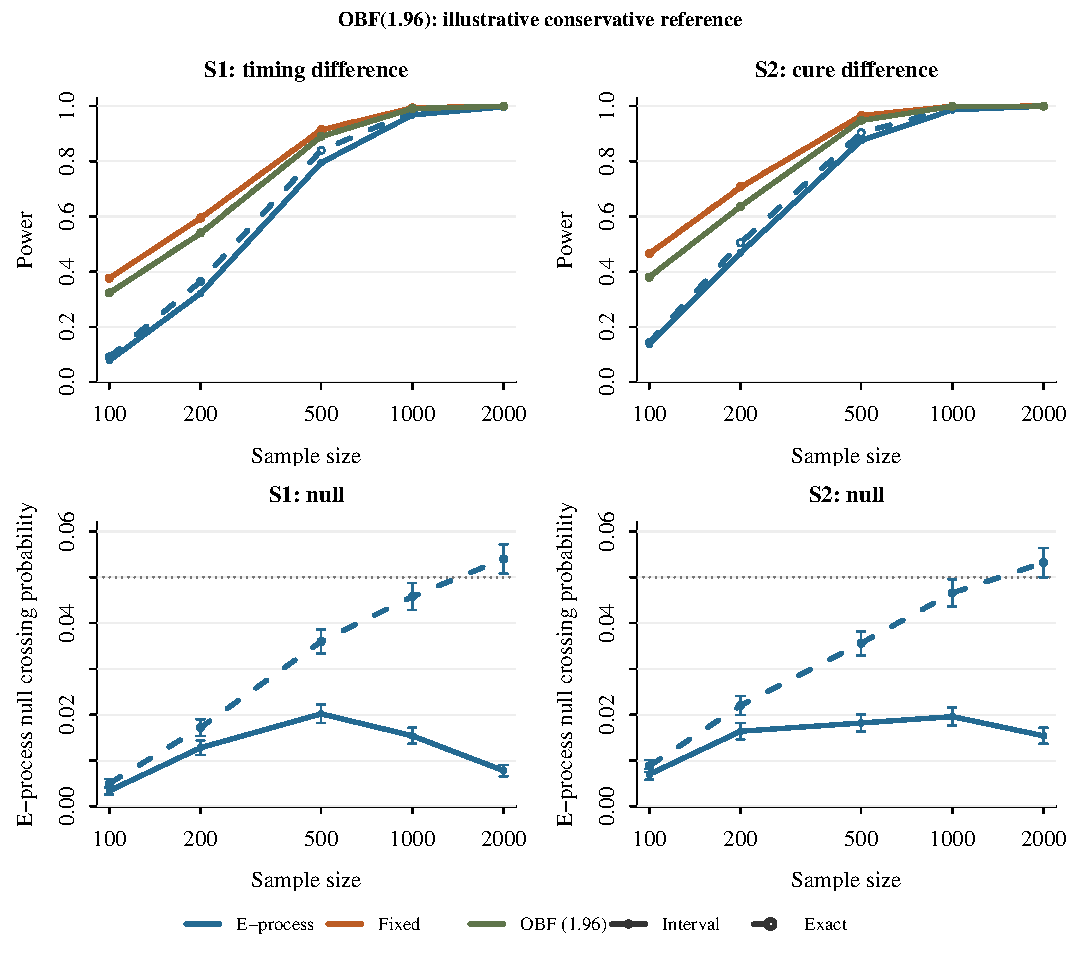
\includegraphics[width=\textwidth]{figures/referee_sim_sample_size.pdf}
\caption{S1/S2 monitoring results with OBF(1.96) as an illustrative conservative reference. Oracle log-growth coefficients are selected under each true alternative. Top: power for the e-process, Fixed and OBF(1.96); the latter is not calibrated to a 5\% rejection probability on the finite schedules. Bottom: e-process null crossing probabilities; bars show one Monte Carlo standard error, and the dotted line is 0.05. Solid lines and filled points denote Interval observation; dashed lines and open points denote Exact observation. The sample-size axis is logarithmic. Each estimate uses 5,000 datasets. Scenario definitions: Table~\ref{tab:simulation-scenarios}.}
\label{fig:simulation-sample-size}
\end{figure}

The OBF null rejection estimates are mostly 0.033--0.042. Its boundary was not calibrated to spend 0.05 over the finite Gaussian information schedule, so comparisons here concern this conservative boundary, not an optimized group-sequential design. In interval-observed S1 at $n=500$, the e-process has median stopping time 2.00 years among rejections, compared with 3.00 for OBF, but its mean capped time is slightly longer, 3.81 versus 3.74 years. Nonrejecting datasets contribute the full planned duration to this mean. Earlier rejection in selected datasets need not reduce expected follow-up. Fixed has known analysis time 8 years in S1 and 10 years in S2 (Table~\ref{tab:primary-performance}).

\begin{samepage}
The null curves also distinguish monitoring schemes. Exact observation provides more event-time updates as the sample size increases; grouped observation retains the fixed annual assessment grid and increases the counts within each update. The grouped null crossing estimates remain well below 0.05 and are not monotone in sample size, whereas the exact estimates approach 0.05 in these designs. Coefficients are also selected separately by sample size. The plots therefore reflect changes in the number of event-time updates, counts within grouped updates and selected coefficients, not a failure of the conditional martingale argument or a theorem about monotone convergence to the nominal level. Across primary designs the estimated e-process null rejection ranges from 0.003 to 0.054, compared with 0.125--0.509 for Repeated; Monte Carlo variation must be considered when interpreting estimates near 0.05.
\par\end{samepage}

\subsection{Sensitivity to assessment spacing, allocation, censoring and stratification}
\label{sec:observation-sensitivity}

The assessment-frequency experiment holds follow-up at 8 years and the event-time model fixed while varying visit spacing over 0.5, 1 and 2 years. It uses susceptible control hazard 0.21, treatment hazard ratio 0.70, cure probability 0.15 in both groups and independent exponential censoring at rate 0.085. The annual-design coefficient selected at $n=500$ is retained at all sample sizes and spacings. Only completed intervals contribute. Thus changing visit spacing changes both when evidence can arrive and how much follow-up remains unassessed before censoring.

At $n=500$, e-process power is 0.615, 0.597 and 0.519 at the three spacings, with conditional median stopping times 2.50, 3.00 and 4.00 years (Figure~\ref{fig:simulation-assessments}). The differences are much smaller near the upper end of the sample-size grid, where power is already high. These results concern the retained annual-design coefficient, not a separate optimum for each schedule. The full grid and the effect-size sensitivity designs are given in Tables~\ref{tab:visit-frequency} and~\ref{tab:effect-size}.

\begin{figure}[H]
\centering
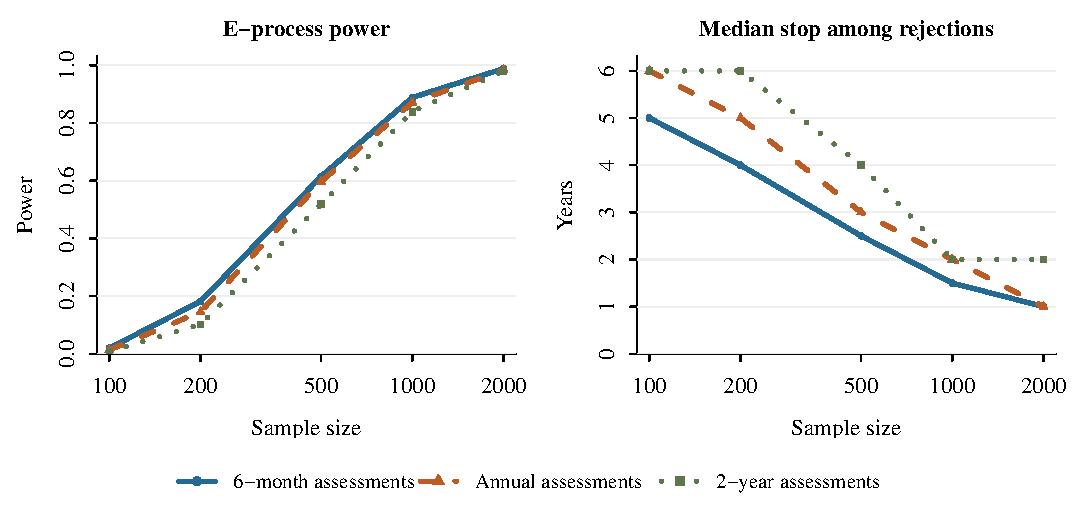
\includegraphics[width=\textwidth]{figures/referee_sim_assessment_frequency.pdf}
\caption{Effect of assessment spacing with a fixed 8-year duration and the same annual-design coefficient. Left: e-process power. Right: median stopping time conditional on rejection, which is not expected study duration. Lines represent 6-month, annual and 2-year assessments. The sample-size axis is logarithmic, and each estimate uses 5,000 alternative datasets.}
\label{fig:simulation-assessments}
\end{figure}

The allocation and censoring grid keeps the coefficient fixed while changing sample size, treatment assignment probability and loss to follow-up (Tables~\ref{tab:design-interval} and~\ref{tab:design-exact}). Its e-process null rejection estimates range from 0.000 to 0.052, compared with 0.115--0.447 for Repeated. A different issue arises in the covariate experiment: treatment assignment favours the lower-risk stratum, and subjects enter at different event-free times. Stratifying the completed-interval comparisons gives null rejection between 0.001 and 0.021; pooling gives 0.179--0.842 (Table~\ref{tab:covariate}). The contrast shows why a valid monitoring rule cannot repair a comparison whose conditional null is wrong. Appendix~\ref{sec:covariate-simulation} gives the entry-conditioned cure model and all design parameters.

\subsection{Combining exact and completed-window records}
\label{sec:mixed-resolution-main}

In S1 and S2, each subject is independently assigned to exact observation with probability $r_{\mathrm{exact}}\in\{0,0.25,0.5,0.75,1\}$, independently of treatment, event time and censoring. The remaining subjects are assessed annually. Under the null, the independent subject records, common stratum survival law and independent censoring satisfy the joint sufficient model in Corollary~\ref{cor:mixed-streams}. The unified analysis combines exact risk-set updates and completed-interval updates, formed within their respective observation subcohorts, in time order. It is compared with using only the exact subcohort, coarsening everyone to annual intervals, and an all-exact benchmark that has additional event-time information. All analyses share the latent datasets. Independent true-alternative pilots choose log-growth coefficients separately for each analysis and fraction; the all-interval and all-exact coefficients are shared across fractions.

At $n=500$ and $r_{\mathrm{exact}}=0.5$, unified power is 0.8190 in S1 and 0.8984 in S2, compared with 0.4924 and 0.6366 when the interval-observed subcohort is discarded. Coarsening the full sample gives 0.7856 and 0.8776. The latter comparison asks whether preserving exact timing compensates for making comparisons within smaller observation subcohorts. Subtracting all-interval power from unified power gives differences of 0.0334 in S1 and 0.0208 in S2, with paired Monte Carlo standard errors 0.00280 and 0.00233, respectively.

At $n=100$ in S1, the unified estimate at the same fraction is 0.0744, below 0.0792 for all-interval observation, a difference of $-0.0048$ with paired Monte Carlo standard error 0.00204. These standard errors condition on the independently selected coefficients and omit variation from repeating the pilot calibration. Each contrast compares separately calibrated procedures with different comparison sets. Exact timing can add information, but smaller risk sets and grouped comparison sets can offset that benefit. Tables~\ref{tab:app-mixed-null} and~\ref{tab:app-mixed-power} retain the complete null and power results; they support examining this tradeoff in the intended study design rather than assuming a fixed ordering.

\section{Exploratory clinical reconstructions}
\label{sec:clinical}

\subsection{Observation models and analysis specification}
\label{sec:application-plan}

The cardiac allograft vasculopathy (CAV) and psoriatic arthritis (PsA) data from \texttt{msm} illustrate evidence calculations after irregular visits have been grouped into working assessment intervals. Follow-up is aligned within patients, rather than monitored prospectively across staggered recruitment. The observation assumptions required for exact validity are not established for either cohort. We therefore use 20 as a reference threshold and interpret the weight and grid comparisons descriptively.

Within each application, every weight uses the same comparison tables, prognostic strata and coefficient mixture. LR is the reference weight; GB, PP, FH, GT and the equal LR--GT mixture assess other working alternatives. GB divides the current table size by the eligible baseline count in its prognostic band. PP, FH with $(\rho,\gamma)=(0,1)$, and GT with $s_{\min}=0.12$ use the band's survival estimate before the current batch. After all tables at time $t$, this estimate is multiplied by $1-\sum_j M_j/\sum_j N_j$, summing over that band's tables at $t$. It is an estimator for the constructed comparisons, not a Kaplan--Meier estimate from the original visits. Each coefficient mixture averages complete processes. Changing $w_j$ at fixed $\eta$ changes the magnitude $\eta w_j$ as well as its temporal emphasis.

Table~\ref{tab:clinical-information} distinguishes retained events from informative comparisons. We call a table informative when its hypergeometric conditional variance is positive, requiring both groups and both event and nonevent observations. A table containing only events contributes no comparative evidence even when both groups are present. Full evidence summaries and observed ranges of $\eta w_j$ appear in Appendix~\ref{sec:clinical-supplement}.

\begin{table}[H]
\centering
\small
\caption{Comparative information after rounding or binning visits. The comparison and event columns show informative/total counts, where informative means positive conditional variance. All 214 CAV detections and 72 PsA progressions are retained at every width, but fewer contribute to a group comparison.}
\label{tab:clinical-information}
\begin{tabular}{llrrrr}
\toprule
Application & Width $q$ & Retained intervals & Monitoring times & Comparisons & Events\\
\midrule
CAV & 0.10 years & 1477 & 95 & 67/521 & 130/214\\
CAV & 0.25 years & 1475 & 51 & 70/329 & 166/214\\
CAV & 0.50 years & 1475 & 31 & 63/257 & 175/214\\
PsA & 3 months & 202 & 7 & 5/16 & 51/72\\
PsA & 6 months & 193 & 4 & 4/8 & 61/72\\
PsA & 12 months & 186 & 2 & 3/4 & 71/72\\
\bottomrule
\end{tabular}
\end{table}

\subsection{Cardiac allograft vasculopathy}
\label{sec:application-cav}

The \texttt{cav} data contain 2,846 records from 622 heart-transplant recipients undergoing approximately yearly angiography \citep{Jackson2011msm,SharplesEtAl2003}. We compare 313 recipients with pretransplant ischaemic heart disease, IHD, group 1, and 270 with idiopathic dilated cardiomyopathy, IDC, group 0. The event is first detected mild, moderate or severe CAV, with 128 IHD and 86 IDC detections. We stratify by sex, baseline recipient age below 45, 45--54 or at least 55 years, and donor age below 30 or at least 30 years. The comparison is prognostic and does not remove residual confounding.

Each event interval runs from the last negative to the first positive angiogram. Death before detected CAV censors follow-up at the last negative angiogram, requiring an assumption of noninformative death that is doubtful in this setting. For width $q$, each endpoint $t$ is rounded to $q\,\mathrm{round}(t/q)$ using R's ties-to-even rule. Intervals with coincident rounded endpoints are omitted; none contains a first CAV detection. A comparison requires agreement of both rounded endpoints and the prognostic categories. Tables ending at rounded time $r$ are combined and inspected at $r+q/2$, after all actual visits assigned to that batch. Exact validity would require a common conditional event probability despite differences between the actual intervals grouped together.

The reference specification uses $q=0.25$ years and equal weights on $\eta\in\{-\log2,-\log1.5,\log1.5,\log2\}$. LR first reaches 20 at 4.38 years, peaks at 369.11 at 5.38 years and ends at 34.69. With the same tables, GT ends at $5.14\times10^{-15}$. The observed GT weights attain the cap $8.33$ in informative comparisons, giving $\eta w_j$ between $-5.776$ and $5.776$, or conditional odds from approximately $0.0031$ to $322.54$. LR uses odds from $0.5$ to $2$. The large difference in terminal evidence therefore compares substantially different alternative magnitudes, as well as different time emphases. Figure~\ref{fig:cav-evidence} also shows declines after earlier threshold crossings. Its vertical scale is linear from zero to one, so values below one remain visible, and logarithmic above one, so large evidence values fit on the same plot. Wider rounding retains more events in informative tables, but changes their composition and the evidence path.

\begin{figure}[H]
\centering
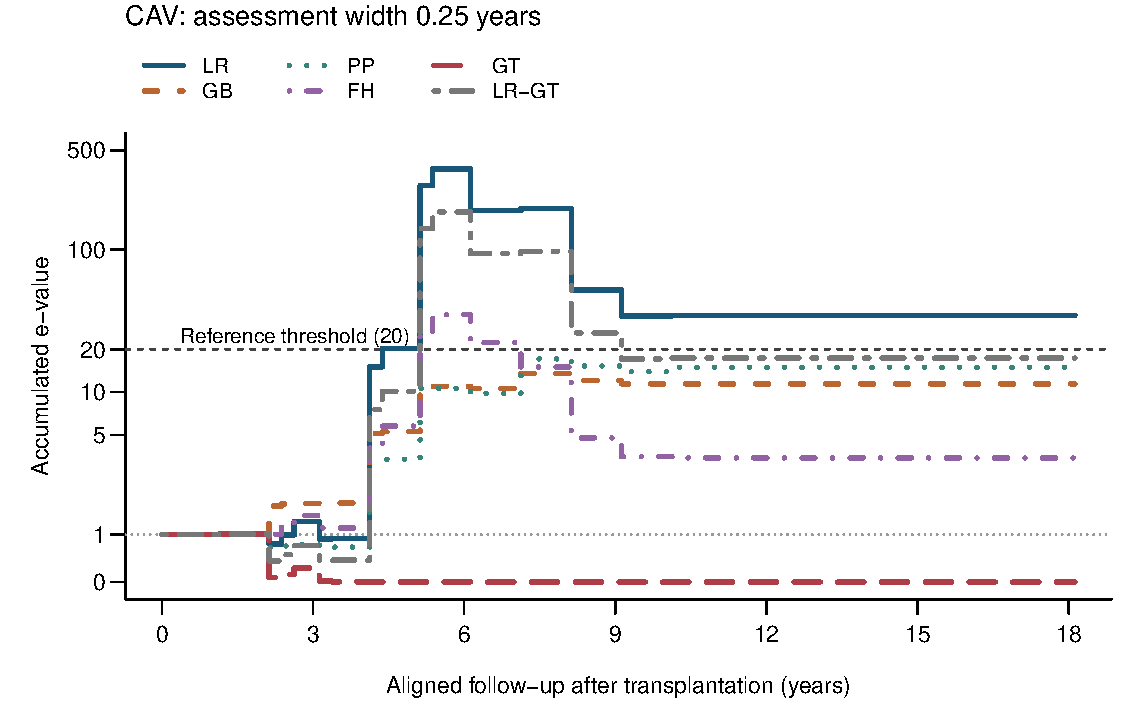
\includegraphics[width=\textwidth]{figures/referee_cav_evidence.pdf}
\caption{Retrospective CAV evidence at $q=0.25$ years under the working common-probability assumption for rounded intervals and noninformative censoring at the last negative angiogram. These assumptions are not established for this cohort. Steps occur at fixed upper bin edges on aligned post-transplant follow-up. The line at 20 is a reference threshold. The vertical scale is linear from 0 to 1 and logarithmic above 1.}
\label{fig:cav-evidence}
\end{figure}

\subsection{Psoriatic-arthritis progression}
\label{sec:application-psor}

The \texttt{psor} data contain 806 clinic observations from 305 patients \citep{Jackson2011msm,GladmanFarewell1999}. Excluding 93 patients with joint damage at their first visit and 27 with missing baseline erythrocyte sedimentation rate (ESR) leaves 185 patients. Of these, 120 have ESR $\geq15$ mm/h, group 0, and 65 have ESR $<15$ mm/h, group 1. First progression to at least one damaged joint occurs in 54 and 18 patients, respectively; 66 and 47 are censored at their final damage-free visit. The comparison adjusts for baseline high effusion, present in only 20 eligible patients, including three with ESR $<15$ mm/h.

Follow-up begins at the first recorded damage-free visit. In each right-closed nominal window $((k-1)q,kq]$, the last visit is selected by time alone. Follow-up stops at the first retained positive state. Because damage states never decrease, each patient with an observed progression retains one event in the same first-positive nominal bin. The selected positive assessment can be later than the original first-positive visit within that bin. Tables group the previous and current nominal bins and high-effusion status, and updates are combined at $kq$. Actual visit times vary within the bins; attendance, loss to follow-up and treatment may depend on disease activity. Common conditional event probabilities are consequently a working assumption. The comparison is observational, with selection at cohort entry and possible residual confounding.

The reference width is six months, within the source study's 6--12-month assessment protocol. The equal mixture uses $\eta=\log(0.50),\log(0.67),\log(0.80)$. The direction follows a published outcome analysis of the same cohort and is outside the optional-monitoring guarantee. Only four of the eight reference tables are informative, as shown in Table~\ref{tab:psa-eight}. In particular, all seven patients in the $(6,12]$-month table progress, so these events contribute a factor of one. LR equals 3.19, 8.25, 11.22 and 11.22 at months 6, 12, 18 and 24. GT equals 23.63 by month 18. Its informative-table weights reach 2.326, with $\eta w_j\in[-1.613,-0.223]$, compared with $[-0.693,-0.223]$ for LR. Thus GT's larger contributions at months 12 and 18 use alternatives with lower group-1 event odds as well as greater late emphasis. Because the weights were compared retrospectively, the GT crossing is descriptive. No weight reaches 20 with three- or twelve-month bins.

\begin{table}[H]
\centering
\small
\caption{The eight six-month PsA comparison tables. Group columns report events/subjects, with $v_j$ the conditional hypergeometric variance. The last columns give the LR and GT mixture multipliers $E_j^{\mathrm{mix}}/E_{j-1}^{\mathrm{mix}}$ in the displayed row order. Only products over all tables ending at one time are monitored; intermediate multipliers depend on the chosen within-batch ordering.}
\label{tab:psa-eight}
\begin{tabular}{lcrrrrr}
\toprule
Window & High & ESR $\geq15$ & ESR $<15$ & $v_j$ & LR & GT\\
(months) & effusion & mm/h & mm/h & & multiplier & multiplier\\
\midrule
$(0,6]$ & No & 32/70 & 14/47 & 6.767 & 3.436 & 3.436\\
$(0,6]$ & Yes & 5/15 & 1/3 & 0.588 & 0.928 & 0.928\\
$(0,12]$ & No & 7/28 & 0/13 & 1.288 & 2.588 & 4.137\\
$(0,12]$ & Yes & 2/2 & 0/0 & 0 & 1 & 1\\
$(6,12]$ & No & 4/4 & 3/3 & 0 & 1 & 1\\
$(0,18]$ & No & 2/4 & 0/2 & 0.356 & 1.360 & 1.792\\
$(6,18]$ & No & 1/1 & 0/0 & 0 & 1 & 1\\
$(0,24]$ & No & 1/1 & 0/0 & 0 & 1 & 1\\
\bottomrule
\end{tabular}
\end{table}

\begin{figure}[H]
\centering
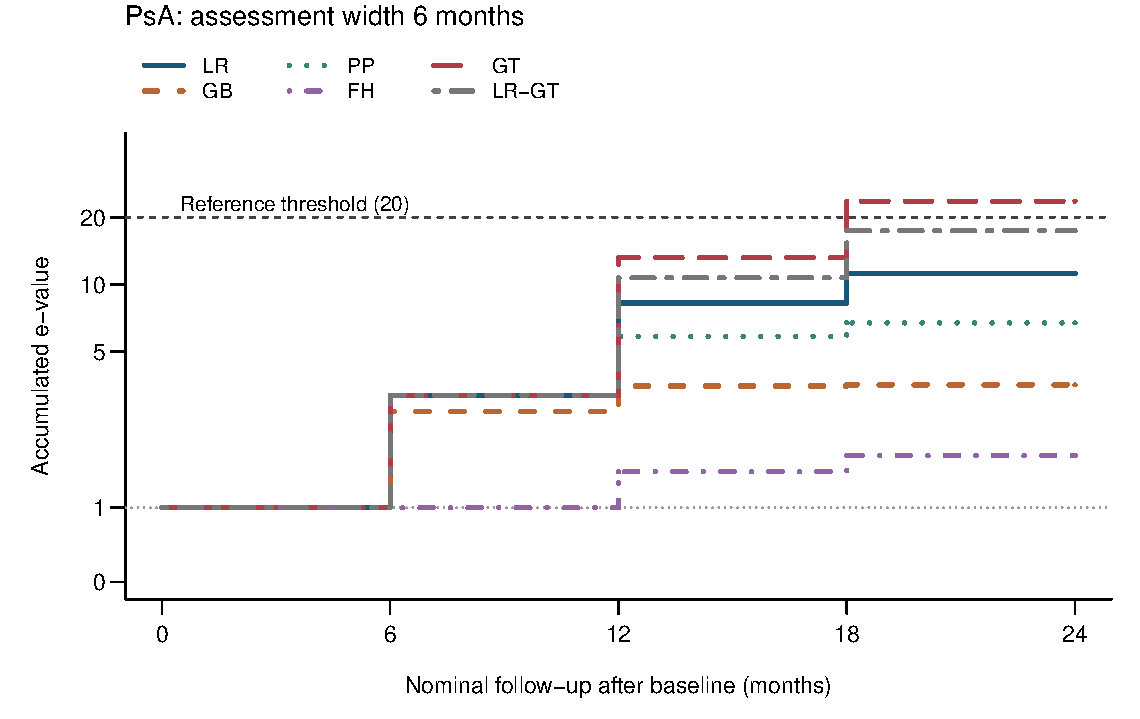
\includegraphics[width=\textwidth]{figures/referee_psa_evidence.pdf}
\caption{Retrospective PsA evidence at $q=6$ months under a working common-probability model for nominal visit bins. That model and noninformative attendance are not established for this cohort; the direction was informed by an earlier analysis of the same outcomes. Evidence is reconstructed on aligned follow-up and inspected at the four nominal assessment times. The line at 20 is a reference threshold. The vertical scale is linear from 0 to 1 and logarithmic above 1.}
\label{fig:psa-evidence}
\end{figure}

\subsection{Stress tests of irregular visits}
\label{sec:clinical-stress-main}

\citet{FayShih2012} study weighted logrank tests for interval-censored data when assessment distributions depend on treatment, using asymptotic arguments and simulation to examine calibration at a fixed analysis. That setting differs from the repeated-monitoring guarantee under Condition~\ref{ass:allocation}.

We applied the actual CAV rounding and PsA visit-binning functions to synthetic visits under equal latent event hazards in the two groups. Each of three visit mechanisms has 2,000 replications. For PsA, making group-1 visits earlier within each nominal window changes the observed LR and GT threshold-crossing frequencies from 0.0085 and 0.0090 on the common grid to 0.0540 and 0.0570. Their 95\% Wilson intervals, $[0.0449,0.0648]$ and $[0.0477,0.0680]$, include 0.05. This shows sensitivity to differential visit timing, without establishing above-nominal crossing probabilities. Group-independent jitter gives 0.0070 and 0.0085, and all CAV estimates remain below 0.05. Appendix~\ref{sec:clinical-stress} specifies the mechanisms and interval-probability diagnostics. These stress tests do not validate either cohort's observation assumptions.

\section{Discussion}
\label{sec:discussion}

Conditional likelihood-ratio normalization permits exact and completed-window comparisons to be monitored in one process when their allocation laws hold given the combined history. The independent-stream corollary supplies one sufficient joint model. The survival-weight specialization connects that process to classical weighted scores, while the fixed-margin local calculation addresses relative score shifts. These results leave the design question of finite-duration rejection probability to the specified alternative, observation scheme and monitoring rule.

Weight choice cannot be separated from the choice of $\eta$. In interval-observed S4 at $n=500$, the normalized Fleming--Harrington specification exceeded LR under both fixed and oracle specifications. In interval-observed S3 at the same sample size, PP exceeded LR under alternative-specific normalization and coefficient selection, but the ordering reversed under fixed specifications. Small positive PP differences remain elsewhere in the fixed-specification grid, so this is not a uniform ordering across sample sizes. The featured comparisons condition on the realized pilots, and neither normalization nor coefficient selection was varied alone. Increasing mean terminal log evidence could also reduce the probability of rejection before follow-up ended. A useful design comparison must therefore specify both the anticipated effects and the performance objective.

Mixture performance also depends on sample size and the chosen objective. At $n=100$, Cmix has higher estimated power than LR in all ten scenario--observation combinations in Table~\ref{tab:app-fixed-design-power}. At $n=2000$ under interval-observed S4, Wmix has higher estimated power than FH, 0.982 versus 0.953, but longer mean capped follow-up, 5.34 versus 5.10 years (Table~\ref{tab:app-fixed-design-stop}). These descriptive comparisons do not give a single preferred mixture across study sizes and performance criteria.

The small-sample power losses relative to the terminal score test were substantial for the specified procedures. For a prespecified terminal sample size, \citet{KoningVanMeer2026} construct an anytime-valid sequence of $[0,1]$-valued tests that agrees with the chosen valid terminal test at that sample size. The e-process allows stopping or continuation without a new type-I error calculation. That flexibility need not be valuable in a study with one feasible analysis and a firm end date. When monitoring is important, design simulations should report rejection probability and mean capped follow-up across plausible alternatives. Stopping medians conditional on rejection describe the successful replications. OBF(1.96) is only an illustrative conservative reference here; quantifying efficiency relative to planned group-sequential monitoring would require a comparator calibrated to the same rejection probability and information schedule.

The clinical analyses expose a separate difficulty. Rounding or binning irregular visits changes which subjects can be compared and can place subjects with different interval event probabilities in the same table. Retaining each first detection does not retain all comparative information: tables with zero conditional variance contribute a factor of one. The clinical weight comparisons also change the magnitude of the conditional-odds alternative, as well as its timing. Their threshold crossings are exploratory descriptions under working observation assumptions, rather than demonstrations of the exact monitoring guarantee for these cohorts.

The method applies when the conditional allocation model is defensible. Residual prognostic heterogeneity within strata, informative attendance and outcome-related censoring can invalidate it. A rejection with a late-emphasis weight does not identify a cured subgroup without further follow-up and assumptions about susceptible subjects' long-term survival \citep{MallerZhou1992}. Prospective use with staggered recruitment must also respect the order in which observations become available; delayed entry on a common risk-time scale is different from aligning each subject's time since entry \citep[Section~8.2]{TerSchureEtAl2024}. Extending the construction to history-dependent visits or continuous-covariate adjustment requires a justified conditional allocation law, rather than only a different weight. These observation-model questions are the principal limitation of applying the procedure beyond common completed windows.

\section*{Data accessibility statement}
Data and code supporting the analyses are available in the accompanying \href{https://github.com/hiendn/Anytime_Valid_Survival_Tests}{GitHub repository}. The reported analyses use the scientific code and data at \href{https://github.com/hiendn/Anytime_Valid_Survival_Tests/tree/025903c484a004cd278c86738f0721d05104c790}{commit \texttt{025903c}}. The round-7 source and an archival PDF build are stored under \href{https://github.com/hiendn/Anytime_Valid_Survival_Tests/tree/manuscript-round7-2026-10-23}{version \texttt{manuscript-round7-2026-10-23}}, with the hashes of those archived artifacts and their verification scope recorded in the repository.

\section*{AI use statement}
OpenAI ChatGPT and Codex were used for exposition, mathematical formulation, proof checking, computational implementation, proofreading, and formatting. The authors take responsibility for all parts of this manuscript.

\renewcommand{\refname}{References}
\begin{thebibliography}{52}

\bibitem[Andersen et~al.(1993)Andersen, Borgan, Gill, and
  Keiding]{AndersenEtAl1993}
Per~Kragh Andersen, Ornulf Borgan, Richard~D. Gill, and Niels Keiding.
\newblock \emph{Statistical Models Based on Counting Processes}.
\newblock Springer, New York, 1993.

\bibitem[Boher et~al.(2024)Boher, Filleron, Sfumato, Bunouf, and Cook]{BoherEtAl2024}
Jean~Marie Boher, Thomas Filleron, Patrick Sfumato, Pierre Bunouf, and Richard~J. Cook.
\newblock Group sequential methods based on supremum logrank statistics under proportional and nonproportional hazards.
\newblock \emph{Statistical Methods in Medical Research}, 33\penalty0 (7):\penalty0 1137--1151, 2024.
\newblock doi:10.1177/09622802241254211.

\bibitem[Brummel and Gillen(2014)]{BrummelGillen2014}
Sean~S. Brummel and Daniel~L. Gillen.
\newblock Flexibly monitoring group sequential survival trials when testing is based upon a weighted log-rank statistic.
\newblock \emph{Sequential Analysis}, 33\penalty0 (1):\penalty0 39--59, 2014.
\newblock doi:10.1080/07474946.2014.856635.

\bibitem[Choe and Ramdas(2026)]{ChoeRamdas2026}
Yo~Joong Choe and Aaditya Ramdas.
\newblock Combining evidence across filtrations.
\newblock \emph{Journal of the Royal Statistical Society Series B: Statistical Methodology}, 88\penalty0 (4):\penalty0 1492--1514, 2026.
\newblock doi:10.1093/jrsssb/qkag058.

\bibitem[Cochran(1954)]{Cochran1954}
William~G. Cochran.
\newblock Some methods for strengthening the common chi-squared tests.
\newblock \emph{Biometrics}, 10\penalty0 (4):\penalty0 417--451, 1954.

\bibitem[Cox(1972)]{Cox1972}
David~R. Cox.
\newblock Regression models and life-tables.
\newblock \emph{Journal of the Royal Statistical Society: Series B},
  34\penalty0 (2):\penalty0 187--220, 1972.

\bibitem[Fay and Shaw(2010)]{FayShaw2010}
Michael~P. Fay and Pamela~A. Shaw.
\newblock Exact and asymptotic weighted logrank tests for interval censored
  data: The interval {R} package.
\newblock \emph{Journal of Statistical Software}, 36\penalty0 (2):\penalty0
  1--34, 2010.

\bibitem[Fay and Shih(2012)]{FayShih2012}
Michael~P. Fay and Joanna~H. Shih.
\newblock Weighted logrank tests for interval censored data when assessment
  times depend on treatment.
\newblock \emph{Statistics in Medicine}, 31\penalty0 (28):\penalty0
  3760--3772, 2012.
\newblock doi:10.1002/sim.5447.

\bibitem[Finkelstein(1986)]{Finkelstein1986}
Dianne~M. Finkelstein.
\newblock A proportional hazards model for interval-censored failure time data.
\newblock \emph{Biometrics}, 42\penalty0 (4):\penalty0 845--854, 1986.

\bibitem[Fleming and Harrington(1991)]{FlemingHarrington1991}
Thomas~R. Fleming and David~P. Harrington.
\newblock \emph{Counting Processes and Survival Analysis}.
\newblock Wiley, New York, 1991.

\bibitem[Fog(2008)]{Fog2008}
Agner Fog.
\newblock Sampling methods for Wallenius' and Fisher's noncentral
  hypergeometric distributions.
\newblock \emph{Communications in Statistics---Simulation and Computation},
  37\penalty0 (2):\penalty0 241--257, 2008.

\bibitem[Gehan(1965)]{Gehan1965}
Edmund~A. Gehan.
\newblock A generalized {Wilcoxon} test for comparing arbitrarily
  singly-censored samples.
\newblock \emph{Biometrika}, 52\penalty0 (1--2):\penalty0 203--223, 1965.

\bibitem[Gill et~al.(1997)Gill, van~der Laan, and
  Robins]{GillVanDerLaanRobins1997}
Richard~D. Gill, Mark~J. van~der Laan, and James~M. Robins.
\newblock Coarsening at random: Characterizations, conjectures,
  counter-examples.
\newblock \emph{State of the Art in Survival Analysis}, pages 255--294, 1997.

\bibitem[Gladman and Farewell(1999)]{GladmanFarewell1999}
Danielle~D. Gladman and Vernon~T. Farewell.
\newblock Progression in psoriatic arthritis: role of time-varying clinical
  indicators.
\newblock \emph{Journal of Rheumatology}, 26\penalty0 (11):\penalty0
  2409--2413, 1999.

\bibitem[Gray and Tsiatis(1989)]{GrayTsiatis1989}
Robert~J. Gray and Anastasios~A. Tsiatis.
\newblock A linear rank test for use when the main interest is in differences
  in cure rates.
\newblock \emph{Biometrics}, 45\penalty0 (3):\penalty0 899--904, 1989.

\bibitem[Harrington and Fleming(1982)]{HarringtonFleming1982}
David~P. Harrington and Thomas~R. Fleming.
\newblock A class of rank test procedures for censored survival data.
\newblock \emph{Biometrika}, 69\penalty0 (3):\penalty0 553--566, 1982.

\bibitem[Heitjan and Rubin(1991)]{HeitjanRubin1991}
Daniel~F. Heitjan and Donald~B. Rubin.
\newblock Ignorability and coarse data.
\newblock \emph{The Annals of Statistics}, 19\penalty0 (4):\penalty0
  2244--2253, 1991.

\bibitem[Jackson(2011)]{Jackson2011msm}
Christopher~H. Jackson.
\newblock Multi-state models for panel data: The \texttt{msm} package for
  \texttt{R}.
\newblock \emph{Journal of Statistical Software}, 38\penalty0 (8):\penalty0
  1--29, 2011.
\newblock doi:10.18637/jss.v038.i08.

\bibitem[Koning and van Meer(2026)]{KoningVanMeer2026}
Nick~W. Koning and Sam van Meer.
\newblock Anytime validity is free: inducing sequential tests.
\newblock \emph{Journal of the Royal Statistical Society Series B: Statistical Methodology}, 88\penalty0 (4):\penalty0 1366--1384, 2026.
\newblock doi:10.1093/jrsssb/qkag050.

\bibitem[Kundu and Sarkar(2021)]{KunduSarkar2021}
Madan~G. Kundu and Jyotirmoy Sarkar.
\newblock On information fraction for {Fleming--Harrington} type weighted log-rank tests in a group-sequential clinical trial design.
\newblock \emph{Statistics in Medicine}, 40\penalty0 (10):\penalty0 2321--2338, 2021.
\newblock doi:10.1002/sim.8905.

\bibitem[Lan and DeMets(1983)]{LanDeMets1983}
K.~K.~Gordon Lan and David~L. DeMets.
\newblock Discrete sequential boundaries for clinical trials.
\newblock \emph{Biometrika}, 70\penalty0 (3):\penalty0 659--663, 1983.

\bibitem[Law and Brookmeyer(1992)]{LawBrookmeyer1992}
C.~G. Law and Ron Brookmeyer.
\newblock Effects of midpoint imputation on the analysis of doubly censored
  data.
\newblock \emph{Statistics in Medicine}, 11\penalty0 (12):\penalty0 1569--1578,
  1992.

\bibitem[Li and Wang(2026)]{LiWang2026}
Zhiguo Li and Xiaofei Wang.
\newblock A powerful and self-adaptive weighted logrank test.
\newblock \emph{Statistics in Medicine}, 45\penalty0 (3--5):\penalty0 e70390, 2026.
\newblock doi:10.1002/sim.70390.

\bibitem[Lin and Le\'on(2017)]{LinLeon2017}
Ray~S. Lin and Larry~F. Le\'on.
\newblock Estimation of treatment effects in weighted log-rank tests.
\newblock \emph{Contemporary Clinical Trials Communications}, 8:\penalty0
  147--155, 2017.
\newblock \url{https://doi.org/10.1016/j.conctc.2017.09.004}.

\bibitem[Maller and Zhou(1992)]{MallerZhou1992}
Ross~A. Maller and S.~Zhou.
\newblock Estimating the proportion of immunes in a censored sample.
\newblock \emph{Biometrika}, 79\penalty0 (4):\penalty0 731--739, 1992.

\bibitem[Mantel(1966)]{Mantel1966}
Nathan Mantel.
\newblock Evaluation of survival data and two new rank order statistics arising
  in its consideration.
\newblock \emph{Cancer Chemotherapy Reports}, 50\penalty0 (3):\penalty0
  163--170, 1966.

\bibitem[Mantel and Haenszel(1959)]{MantelHaenszel1959}
Nathan Mantel and William Haenszel.
\newblock Statistical aspects of the analysis of data from retrospective
  studies of disease.
\newblock \emph{Journal of the National Cancer Institute}, 22\penalty0
  (4):\penalty0 719--748, 1959.

\bibitem[O'Brien and Fleming(1979)]{OBrienFleming1979}
Peter~C. O'Brien and Thomas~R. Fleming.
\newblock A multiple testing procedure for clinical trials.
\newblock \emph{Biometrics}, 35\penalty0 (3):\penalty0 549--556, 1979.

\bibitem[Ramdas and Wang(2025)]{RamdasWang2025}
Aaditya Ramdas and Ruodu Wang.
\newblock Hypothesis testing with e-values.
\newblock \emph{Foundations and Trends in Statistics}, 1\penalty0
  (1--2):\penalty0 1--390, 2025.

\bibitem[Robins and Finkelstein(2000)]{RobinsFinkelstein2000}
James~M. Robins and Dianne~M. Finkelstein.
\newblock Correcting for noncompliance and dependent censoring in an {AIDS}
  clinical trial with inverse probability of censoring weighted log-rank tests.
\newblock \emph{Biometrics}, 56\penalty0 (3):\penalty0 779--788, 2000.

\bibitem[Sharples et~al.(2003)Sharples, Jackson, Parameshwar, Wallwork, and
  Large]{SharplesEtAl2003}
Linda~D. Sharples, Christopher~H. Jackson, Jayan Parameshwar, John Wallwork,
  and Stephen~R. Large.
\newblock Diagnostic accuracy of coronary angiography and risk factors for
  post-heart-transplant cardiac allograft vasculopathy.
\newblock \emph{Transplantation}, 76\penalty0 (4):\penalty0 679--682, 2003.
\newblock doi:10.1097/01.TP.0000071200.37399.1D.

\bibitem[Slud(1984)]{Slud1984}
Eric~V. Slud.
\newblock Sequential linear rank tests for two-sample censored survival data.
\newblock \emph{The Annals of Statistics}, 12\penalty0 (2):\penalty0 551--571,
  1984.

\bibitem[Sun(1996)]{Sun1996}
Jianguo Sun.
\newblock A non-parametric test for interval-censored failure time data with
  application to {AIDS} studies.
\newblock \emph{Statistics in Medicine}, 15\penalty0 (13):\penalty0 1387--1395,
  1996.

\bibitem[Sun(2006)]{Sun2006}
Jianguo Sun.
\newblock \emph{The Statistical Analysis of Interval-Censored Failure Time
  Data}.
\newblock Springer, New York, 2006.

\bibitem[ter Schure et~al.(2024)ter Schure, P\'erez-Ortiz, Ly, and
  Gr\"unwald]{TerSchureEtAl2024}
Judith ter Schure, Muriel~F. P\'erez-Ortiz, Alexander Ly, and Peter~D.
  Gr\"unwald.
\newblock The anytime-valid logrank test: Error control under continuous
  monitoring with unlimited horizon.
\newblock \emph{The New England Journal of Statistics in Data Science},
  2:\penalty0 190--214, 2024.

\bibitem[Turnbull(1976)]{Turnbull1976}
Bruce~W. Turnbull.
\newblock The empirical distribution function with arbitrarily grouped,
  censored and truncated data.
\newblock \emph{Journal of the Royal Statistical Society: Series B},
  38\penalty0 (3):\penalty0 290--295, 1976.

\bibitem[Turner and Gr\"unwald(2023)]{TurnerGrunwald2023}
Rosanne~J. Turner and Peter~D. Gr\"unwald.
\newblock Safe sequential testing and effect estimation in stratified count
  data.
\newblock In \emph{Proceedings of the 26th International Conference on
  Artificial Intelligence and Statistics}, volume 206 of \emph{Proceedings of
  Machine Learning Research}, pages 4880--4893, 2023.

\bibitem[Ville(1939)]{Ville1939}
Jean Ville.
\newblock \emph{\'Etude critique de la notion de collectif}.
\newblock Gauthier-Villars, Paris, 1939.

\bibitem[Vovk and Wang(2021)]{VovkWang2021}
Vladimir Vovk and Ruodu Wang.
\newblock E-values: Calibration, combination and applications.
\newblock \emph{The Annals of Statistics}, 49\penalty0 (3):\penalty0
  1736--1754, 2021.

\bibitem[Wang et~al.(2021)Wang, Luo, and Zheng]{WangLuoZheng2021}
Lili Wang, Xiaodong Luo, and Cheng Zheng.
\newblock A simulation-free group sequential design with max-combo tests in the presence of non-proportional hazards.
\newblock \emph{Pharmaceutical Statistics}, 20\penalty0 (4):\penalty0 879--897, 2021.
\newblock doi:10.1002/pst.2116.

\bibitem[Zhao et~al.(2008)Zhao, Zhao, Sun, and Kim]{ZhaoEtAl2008}
Xingqiu Zhao, Qiang Zhao, Jianguo Sun, and Jong~S. Kim.
\newblock Generalized log-rank tests for partly interval-censored failure time
  data.
\newblock \emph{Biometrical Journal}, 50\penalty0 (3):\penalty0 375--385, 2008.

\end{thebibliography}

\appendix
\numberwithin{equation}{section}
\numberwithin{table}{section}
\numberwithin{figure}{section}

\section{Proofs and additional theoretical results}
\label{app:proofs}

The notation follows Section~\ref{sec:methods}.

\subsection{Probability-space and observation-record conventions}
\label{app:formal-setup}

All random objects are measurable on a common space $(\Omega,\mathfrak F)$ under a family of probability measures $\mathcal P$, with $\mathcal P_0\subseteq\mathcal P$ the conditional null family in Section~\ref{sec:methods}. Subject indices lie in $\mathsf I_n=\{1,\ldots,n\}$, group labels in $\{0,1\}$, baseline covariates in a Borel subset $\mathcal X\subseteq\mathbb R^p$, and event and right-censoring times in $(0,\infty]$. The fixed stratification map $\mathsf s:\mathcal X\to\{1,\ldots,K_X\}$ is measurable. These variables, entry times, examination times and comparison sets are measurable, and the discrete observation filtration is contained in $\mathfrak F$.

An interval record $(L_i,R_i]$ satisfies $0\leq L_i<R_i\leq\infty$ and $L_i<T_i\leq R_i$. It includes left censoring when $L_i=0$, $R_i<\infty$, and right censoring when $R_i=\infty$. An exact record gives $T_i$ itself. Under exact observation with right censoring, write
\[
 U_i=\min(T_i,C_i),\qquad
 \Delta_i=\mathbf 1\{T_i<\infty,\ T_i\leq C_i\}.
\]
Thus $\Delta_i=1$ records an event, including an event--censoring tie; finite $U_i$ with $\Delta_i=0$ records $(U_i,\infty]$. A random index $\tau\in\mathbb N_0\cup\{\infty\}$ is a stopping time when $\{\tau\leq j\}\in\mathfrak F_j$ for every $j$. Quantities determined by completed earlier updates are $\mathfrak F_{j-1}$-measurable; exact-event risk-set weights evaluated before the jump are predictable for the continuous-time filtration used below.


\subsection{Proof of anytime validity}

\begin{proof}[Proof of Theorem~\ref{thm:master}]
The event set, margins and numerator kernel are $\mathfrak F_j$-measurable, so $Y_j$ and $e_j$ are $\mathfrak F_j$-measurable. The denominator is positive on $\mathcal Y_j$.
Under Condition~\ref{ass:allocation}, there are $\binom{N_j}{M_j}$ equiprobable event subsets. Exactly $\binom{N_{1j}}{y}\binom{N_{0j}}{M_j-y}$ contain $y$ treatment subjects, which gives \eqref{eq:null-pmf}. Therefore, conditionally on $\mathfrak G_j$, $Y_j$ has mass function $p_{0j}$, and
\[
 \mathbb E_0\left(e_j\mid\mathfrak G_j\right)
 =\sum_{y\in\mathcal Y_j}p_{0j}(y)\frac{q_j(y)}{p_{0j}(y)}
 =\sum_{y\in\mathcal Y_j}q_j(y)=1.
\]
By iterated conditional expectation,
\[
 \mathbb E_0\left(e_j\mid\mathfrak F_{j-1}\right)=1.
\]
Because $E_{j-1}$ is $\mathfrak F_{j-1}$-measurable,
\[
 \mathbb E_0\left(E_j\mid\mathfrak F_{j-1}\right)
 =E_{j-1}\mathbb E_0\left(e_j\mid\mathfrak F_{j-1}\right)=E_{j-1}.
\]
The process is nonnegative and starts at one. Taking expectations inductively gives $\mathbb E_0(E_j)=1$, so every finite-time value is integrable. Ville's maximal inequality gives \eqref{eq:ville-bound}.
\end{proof}

\begin{corollary}[E-value at a stopping time]
\label{cor:app-stopping}
Let $\tau:\Omega\to\mathbb N_0\cup\{\infty\}$ be an almost surely finite stopping time for $(\mathfrak F_J)$, meaning that $\{\omega\in\Omega:\tau(\omega)\leq J\}\in\mathfrak F_J$ for every $J$. Then $\mathbb E_0(E_\tau)\leq1$ for every $\mathbb P_0\in\mathcal P_0$.
\end{corollary}

\begin{proof}
For each $m$, optional sampling at the bounded time $\tau\wedge m$ gives $\mathbb E_0(E_{\tau\wedge m})=1$. Since $\tau<\infty$ almost surely, $E_{\tau\wedge m}\to E_\tau$ almost surely. Fatou's lemma yields
\[
 \mathbb E_0(E_\tau)\leq\liminf_{m\to\infty}\mathbb E_0(E_{\tau\wedge m})=1.
\]
\end{proof}



\subsection{Proof of the score identity and local expansion}

The pathwise expansion in Section~\ref{sec:theory} applies to the realized finite sequence of tables. The triangular-array results below are ancillary: their deterministic conditional laws and weights isolate the additional assumptions needed for a Gaussian limit. They do not establish a central limit theorem for general random risk sets or adaptive weights.

For the factor in \eqref{eq:weighted-factor}, write
\[
 \psi_j(u)=\log\mathbb E_0\left\{\exp\left(uY_j\right)\mid\mathfrak G_j\right\}
\]
so that
\[
 \log e_j^{(w)}(\eta)=\eta w_jY_j-\psi_j(\eta w_j).
\]

\begin{proof}[Proof of Theorem~\ref{thm:score}]
Differentiation gives
\[
 \frac{\partial}{\partial\eta}\log e_j^{(w)}(\eta)
 =w_j\left\{Y_j-\psi_j'(\eta w_j)\right\}.
\]
At zero, $\psi_j'(0)=\mathbb E_0(Y_j\mid\mathfrak G_j)=\mu_j$, the hypergeometric mean. A second differentiation gives
\[
 -\frac{\partial^2}{\partial\eta^2}\log e_j^{(w)}(\eta)
 =w_j^2\psi_j''(\eta w_j).
\]
At zero, $\psi_j''(0)=\mathrm{Var}_0(Y_j\mid\mathfrak G_j)=v_j$. Summing over $j$ proves both identities.

For the variance interpretation in the main text, let $D_j=w_j(Y_j-\mu_j)$. Then $\mathbb E_0(D_j\mid\mathfrak G_j)=0$ and $\mathbb E_0(D_j^2\mid\mathfrak G_j)=w_j^2v_j$. With the refined filtration $\mathfrak J_{2j-2}=\mathfrak F_{j-1}$, $\mathfrak J_{2j-1}=\mathfrak G_j$ and $\mathfrak J_{2j}=\mathfrak F_j$, the cumulative score held constant at odd indices is a martingale. Its predictable quadratic variation at index $2J$ is therefore $\sum_{j=1}^J w_j^2v_j$. Moreover, for $j<k$,
\[
 \mathbb E_0(D_jD_k)
 =\mathbb E_0\left\{D_j\mathbb E_0(D_k\mid\mathfrak F_{k-1})\right\}=0,
\]
where iterated expectation gives $\mathbb E_0(D_k\mid\mathfrak F_{k-1})=0$. Hence square integrability implies
\[
 \mathrm{Var}_0\left(\sum_{j=1}^{J}D_j\right)
 =\sum_{j=1}^J\mathbb E_0(D_j^2)
 =\mathbb E_0\left(\sum_{j=1}^J w_j^2v_j\right).
\]
\end{proof}

\begin{proposition}[Local expansion]
\label{prop:local-expansion}
For each $J$, let $Y_{J,1},\ldots,Y_{J,J}$ be adapted to a filtration $(\mathfrak H_{J,j})_{j=0}^J$. Under $\mathbb P_0$, suppose the conditional law of $Y_{J,j}$ given $\mathfrak H_{J,j-1}$ is a deterministic finite-support distribution with cumulant function
\[
 \psi_{J,j}(u)=\log\mathbb E_0\left\{\exp(uY_{J,j})\mid\mathfrak H_{J,j-1}\right\},
\]
and write $\mu_{J,j}=\psi_{J,j}'(0)$ and $v_{J,j}=\psi_{J,j}''(0)$. Let $w_{J,j}$ be deterministic and define
\[
 V_J=\sum_{j=1}^J w_{J,j}^2v_{J,j},
 \qquad
 Z_J=V_J^{-1/2}\sum_{j=1}^J w_{J,j}(Y_{J,j}-\mu_{J,j}),
\]
where $V_J\to\infty$ and the normalized quantities are defined for $J$ with $V_J>0$. Suppose, for every fixed $c>0$,
\[
 V_J^{-3/2}\sum_{j=1}^J |w_{J,j}|^3
 \sup_{|u|\leq c|w_{J,j}|/\sqrt{V_J}}|\psi_{J,j}'''(u)|
 \longrightarrow0.
\]
For
\[
 E_J^\triangle(\eta)=
 \prod_{j=1}^J
 \exp\left\{\eta w_{J,j}Y_{J,j}-\psi_{J,j}(\eta w_{J,j})\right\}
\]
and the prespecified local sequence $\eta_J=a/\sqrt{V_J}$, with fixed $a\in\mathbb R$,
\[
 \log E_J^\triangle(\eta_J)=aZ_J-a^2/2+o(1).
\]
\end{proposition}

\begin{proof}
For each $j$, Taylor's theorem gives
\[
 \psi_{J,j}(\eta_{J}w_{J,j})
 =\psi_{J,j}(0)+\eta_{J}w_{J,j}\psi_{J,j}'(0)
  +\frac{\eta_J^2w_{J,j}^2}{2}\psi_{J,j}''(0)+R_{J,j},
\]
where
\[
 |R_{J,j}|\leq \frac{|\eta_{J}w_{J,j}|^3}{6}
 \sup_{|u|\leq |a||w_{J,j}|/\sqrt{V_J}}|\psi_{J,j}'''(u)|.
\]
Since $\psi_{J,j}(0)=0$, $\psi_{J,j}'(0)=\mu_{J,j}$ and $\psi_{J,j}''(0)=v_{J,j}$,
\begin{align*}
 \log E_J^\triangle(\eta_J)
 &=\eta_J\sum_{j=1}^J w_{J,j}(Y_{J,j}-\mu_{J,j})
   -\frac{\eta_J^2}{2}\sum_{j=1}^J w_{J,j}^2v_{J,j}
   -\sum_{j=1}^{J}R_{J,j}\\
 &=aZ_J-\frac{a^2}{2}-\sum_{j=1}^{J}R_{J,j}.
\end{align*}
If $a=0$, the result is immediate. If $a\neq0$, the third-derivative condition with $c=|a|$ implies $\sum_{j=1}^J|R_{J,j}|\to0$.
\end{proof}

\begin{corollary}[Gaussian limit under a score central limit theorem]
\label{cor:local-gaussian}
Under the conditions of Proposition~\ref{prop:local-expansion}, if $Z_J\Rightarrow\mathrm{N}(0,1)$ under $\mathbb P_0$, then
\[
 \log E_J^\triangle(\eta_J)\Rightarrow\mathrm{N}\left(-a^2/2,a^2\right).
\]
\end{corollary}

\begin{proof}
Apply Slutsky's theorem to Proposition~\ref{prop:local-expansion}.
\end{proof}

\subsection{Sufficient conditions for exact-event updates}

Let $(\mathfrak F_t^{\mathrm{ex}})_{t\geq0}$ be a filtration satisfying the usual conditions. Let $N_i(t)$ be a simple $\mathfrak F_t^{\mathrm{ex}}$-adapted observed event counting process and $R_i(t)$ an $\mathfrak F_t^{\mathrm{ex}}$-predictable at-risk indicator. The filtration includes the baseline covariates, group labels and previously observed information from all strata. Fix one monitoring and covariate stratum and set $N_i=R_i=0$ for subjects outside it. This is the standard multiplicative-intensity formulation \citep{AndersenEtAl1993,FlemingHarrington1991,TerSchureEtAl2024}.

\begin{condition}[Common null intensity]
\label{ass:common-intensity}
For every $\mathbb P_0\in\mathcal P_0$, the multivariate counting process is nonexplosive on every finite time interval, distinct subjects have no simultaneous event jumps, and $N_i$ has compensator
\[
 \Gamma_i(t)=\int_0^tR_i(s)\lambda(s)\,\mathrm ds
\]
for a common nonnegative $\mathfrak F_t^{\mathrm{ex}}$-predictable process $\lambda$, which may depend on $\mathbb P_0$.
\end{condition}

Let $N_\cdot=\sum_{i=1}^nN_i$, let $T_k^{\mathrm{ex}}$ be its $k$th finite jump time, and let $I_k\in\{1,\ldots,n\}$ be the index of the unique subject whose process jumps at $T_k^{\mathrm{ex}}$. We call $I_k$ the \emph{mark} of this observed failure.

For a stopping time $T$, we use the pre-jump convention
\[
 \mathfrak F^{\mathrm{ex}}_{T-}
 =\sigma\bigl(\mathfrak F^{\mathrm{ex}}_0,
   \{A\cap\{t<T\}:t\geq0,\ A\in\mathfrak F^{\mathrm{ex}}_t\}\bigr).
\]
In this convention $T$ is already measurable in $\mathfrak F^{\mathrm{ex}}_{T-}$; the displayed conditioning on its time below makes the intended information explicit. The marked-process compensator argument uses the standard predictable-compensator framework of \citet{AndersenEtAl1993,FlemingHarrington1991}.

\begin{proposition}[Uniform mark law for an exact failure]
\label{prop:exact-mark}
Under Condition~\ref{ass:common-intensity}, on the event that $T_k^{\mathrm{ex}}<\infty$ and the total risk-set intensity at $T_k^{\mathrm{ex}}$ is positive,
\[
 \mathbb P_0\left(I_k=i\mid
 \mathfrak F_{T_k^{\mathrm{ex}}-}^{\mathrm{ex}}\vee\sigma(T_k^{\mathrm{ex}})\right)
 =\frac{R_i(T_k^{\mathrm{ex}})}{\sum_{r=1}^nR_r(T_k^{\mathrm{ex}})}.
\]
Thus the mark is uniform over the current risk set
\[
 \mathsf R(T_k^{\mathrm{ex}})=\left\{i\in\{1,\ldots,n\}:R_i(T_k^{\mathrm{ex}})=1\right\}.
\]
\end{proposition}

\begin{proof}
Regard the observed events as a marked point process on the product of time and the finite mark space $\{1,\ldots,n\}$. Under Condition~\ref{ass:common-intensity}, its predictable compensator measure is
\[
 \nu(\mathrm dt,\{i\})=R_i(t)\lambda(t)\,\mathrm dt,
\]
with ground compensator
\[
 \nu_\cdot(\mathrm dt)=\lambda(t)\sum_{r=1}^nR_r(t)\,\mathrm dt.
\]
Write
\[
 \pi_i(t)=\frac{R_i(t)}{\sum_{r=1}^nR_r(t)}
\]
when the denominator is positive, and set $\pi_i(t)=0$ otherwise. For any bounded nonnegative predictable $H$, the compensator identities, with the predictable selector $\mathbf 1\{N_\cdot(t-)=k-1\}$, give
\begin{align*}
 &\mathbb E_0\left[H(T_k^{\mathrm{ex}})\mathbf 1\{T_k^{\mathrm{ex}}<\infty,I_k=i\}\right]\\*
 &\quad=\mathbb E_0\int_0^\infty
 H(t)\mathbf 1\{N_\cdot(t-)=k-1\}R_i(t)\lambda(t)\,\mathrm dt\\*
 &\quad=\mathbb E_0\int_0^\infty
 H(t)\mathbf 1\{N_\cdot(t-)=k-1\}\pi_i(t)
 \lambda(t)\sum_{r=1}^nR_r(t)\,\mathrm dt\\*
 &\quad=\mathbb E_0\left[H(T_k^{\mathrm{ex}})\mathbf 1\{T_k^{\mathrm{ex}}<\infty\}
 \pi_i(T_k^{\mathrm{ex}})\right].
\end{align*}
The identities may first be applied up to bounded times and localizing times and then extended by monotone convergence. Indicators of the form $H(t)=\mathbf 1_A\mathbf 1\{t>s\}$, with $A\in\mathfrak F_s^{\mathrm{ex}}$, together with initial measurable indicators, generate $\mathfrak F_{T_k^{\mathrm{ex}}-}^{\mathrm{ex}}$ upon evaluation at $T_k^{\mathrm{ex}}$. A monotone-class argument therefore identifies $\pi_i(T_k^{\mathrm{ex}})$ as the conditional mark probability on $\{T_k^{\mathrm{ex}}<\infty\}$. The jump time itself is measurable with respect to this pre-jump sigma-algebra. Cancelling the common positive intensity yields the asserted uniform distribution on the current stratum's risk set.
\end{proof}

Suppose update $j$ corresponds to $T_k^{\mathrm{ex}}$, with $\mathsf R_j=\mathsf R(T_k^{\mathrm{ex}})$. If
\[
 \mathfrak G_j\subseteq
 \mathfrak F_{T_k^{\mathrm{ex}}-}^{\mathrm{ex}}\vee\sigma(T_k^{\mathrm{ex}}),
\]
then the tower property and $\mathfrak G_j$-measurability of the risk set give
\[
 \mathbb P_0(I_k=i\mid\mathfrak G_j)
 =\frac{\mathbf 1\{i\in\mathsf R_j\}}{N_j}.
\]
Summing over treated subjects gives the $M_j=1$ specialization of \eqref{eq:null-pmf}. If $\mathfrak G_j$ also contains allocations processed in other strata at the same time, the uniform law must hold conditional on those allocations as well; the common-intensity condition alone does not establish this stronger statement.

When $M_j=1$ and $w_j=1$, the normalising constant in \eqref{eq:tilted-pmf} is
\[
 \frac{N_{0j}+e^\eta N_{1j}}{N_j}.
\]
The resulting e-factor is
\[
 e_j(\eta)=
 \begin{cases}
 \dfrac{e^\eta N_j}{N_{0j}+e^\eta N_{1j}},&Y_j=1,\\[6pt]
 \dfrac{N_j}{N_{0j}+e^\eta N_{1j}},&Y_j=0,
 \end{cases}
\]
which is the explicit $M_j=1$ specialization of \eqref{eq:weighted-factor}.

\subsection{Sufficient conditions for interval-censored and left-censored updates}

For a completed interval $(\ell_j,r_j]$, let
\[
 D_{ij}=\mathbf 1\{\ell_j<T_i\leq r_j\},\qquad i\in\mathsf R_j.
\]
If $(D_{ij}:i\in\mathsf R_j)$ is exchangeable conditional on $\mathfrak K_j$, then every binary vector with the same number of ones has the same conditional probability. Since $M_j=\sum_{i\in\mathsf R_j}D_{ij}$, conditioning further on $M_j=m$ makes every size-$m$ event subset equiprobable and establishes Condition~\ref{ass:allocation}.

Under the stronger independent-Bernoulli version of \eqref{eq:common-panel-prob}, for every $\mathsf A\subseteq\mathsf R_j$ with $|\mathsf A|=m$,
\[
 \mathbb P_0\left(\mathsf A_j=\mathsf A\mid\mathfrak K_j\right)
 =p_j^m(1-p_j)^{N_j-m}.
\]
The same fixed-total conditioning therefore applies.

In the basic interval assessment model, let $S$ denote the common stratum-specific population survival function. In the absence of additional history-dependent heterogeneity, a subject known event-free at $\ell_j$ has, provided $S(\ell_j)>0$,
\[
 p_j=1-\frac{S(r_j)}{S(\ell_j)}.
\]
The formula remains valid when $\lim_{t\to\infty}S(t)>0$ because of a cure fraction. For $\ell_j=0$, $S(0)=1$ and $p_j=1-S(r_j)$.

\subsection{A sufficient independent-completion model}

Let
\[
 \mathfrak L_j=\mathfrak F_{j-1}\vee\sigma(O_j)
\]
and suppose the preselection set $\widetilde{\mathsf R}_j$ of subjects known event-free at $\ell_j$ is $\mathfrak L_j$-measurable. For $i\in\widetilde{\mathsf R}_j$, define
\[
 D_{ij}=\mathbf 1\{\ell_j<T_i\leq r_j\},
 \qquad
 B_{ij}=\mathbf 1\{\text{subject $i$ is observed through $r_j$}\},
\]
and set
\[
 \mathsf R_j=\left\{i\in\widetilde{\mathsf R}_j:B_{ij}=1\right\}.
\]
Given the $\mathfrak L_j$-measurable set $\widetilde{\mathsf R}_j$, the random set $\mathsf R_j$ determines the vector $(B_{ij}:i\in\widetilde{\mathsf R}_j)$. Hence the sigma-algebra $\mathfrak K_j$, which records the information before adding the current event total in Section~\ref{sec:information-flow}, satisfies
\[
 \mathfrak K_j=\mathfrak L_j\vee\sigma(\mathsf R_j).
\]

\begin{proposition}[Independent censoring preserves the interval law]
\label{prop:right-censor}
Conditionally on $\mathfrak L_j$, suppose the pairs $(D_{ij},B_{ij})$, indexed by $i\in\widetilde{\mathsf R}_j$, are independent across subjects, each $D_{ij}$ is Bernoulli with a common $\mathfrak L_j$-measurable probability $p_j$, and $D_{ij}$ is conditionally independent of $B_{ij}$ within each pair. Then, conditionally on $\mathfrak K_j$, the retained indicators $(D_{ij}:i\in\mathsf R_j)$ are independent $\mathrm{Bernoulli}(p_j)$. Hence Condition~\ref{ass:allocation} holds after conditioning on $M_j$.
\end{proposition}

\begin{proof}
For each subject and $d\in\{0,1\}$, conditional independence gives
\[
 \mathbb P_0\left(D_{ij}=d\mid B_{ij},\mathfrak L_j\right)
 =\mathbb P_0\left(D_{ij}=d\mid\mathfrak L_j\right).
\]
Conditional independence of the pairs implies that conditioning on the complete vector $(B_{ij}:i\in\widetilde{\mathsf R}_j)$ preserves the product form of the conditional law of the $D_{ij}$. Restricting that product to the indices with $B_{ij}=1$ yields independent $\mathrm{Bernoulli}(p_j)$ indicators conditional on $\mathfrak K_j$. The fixed-total argument from the preceding subsection then gives the hypergeometric allocation law.
\end{proof}

\subsection{A sufficient joint model for mixed observations}

\citet{ChoeRamdas2026} study generic adjustment of e-processes across filtrations. The sufficient model below instead establishes the conditional allocation law directly in the merged release filtration.

\begin{corollary}[Independent observation streams]
\label{cor:mixed-streams}
Condition on baseline information $\mathfrak B$ containing treatment labels, prognostic strata and a partition into finitely many streams indexed jointly by observation regime and monitoring/prognostic stratum. Suppose the complete underlying prospective record sigma-algebras $\mathfrak Z_s$, including any local release randomization, are conditionally independent given $\mathfrak B$. All own-stream filtrations contain $\mathfrak B$ and are contained in $\mathfrak B\vee\mathfrak Z_s$.

In each exact stream, assume Condition~\ref{ass:common-intensity} for its own filtration and use preallocation information
$\mathfrak H_{sk}=\mathfrak F^s_{T_{sk}-}\vee\sigma(T_{sk})$ at its $k$th failure. In each grouped stream, use prospective fixed common windows on a locally finite calendar and assume the pair-independence, common-probability and independent-completion hypotheses of Proposition~\ref{prop:right-censor} given its own preselection history $\mathfrak L_{sk}$, before retention. Use $\mathfrak H_{sk}=\mathfrak L_{sk}\vee\sigma(\mathsf R_{sk},M_{sk})$. In both cases the release time $T_{sk}$ and margins are $\mathfrak H_{sk}$-measurable.

Form comparisons within streams, count each event once, and merge releases chronologically with a tie order fixed before the relevant allocations. Each stream releases at most one table at a time. The combined release filtration uses only baseline information, the permitted own-stream histories and current margins, and already released records from other streams. More precisely, if $C_{jsk}$ is the event that candidate $(s,k)$ occupies merged update $j$, require
\[
 C_{jsk}\in\mathfrak D_{sk},\qquad
 A\cap C_{jsk}\in\mathfrak D_{sk}\quad(A\in\mathfrak G_j),
 \qquad
 \mathfrak D_{sk}=\mathfrak H_{sk}\vee\bigvee_{r\ne s}\mathfrak Z_r.
\]
Weights for a simultaneous release are fixed before its allocations are used. Then every finite merged update satisfies Condition~\ref{ass:allocation}, and Theorem~\ref{thm:master} applies.
\end{corollary}

\begin{proof}
For a nonexistent candidate, set $T_{sk}=\infty$, $\mathsf R_{sk}=\mathsf A_{sk}=\varnothing$ and $M_{sk}=0$, with $\binom00=1$. After the last genuine merged update, use the same trivial empty table; its allocation law is immediate and its factor is one. For a deterministic subject subset $a\subseteq\mathsf I_n$, the exact-mark and independent-completion propositions give
\[
 \mathbb P_0(\mathsf A_{sk}=a\mid\mathfrak H_{sk})
 =K_{sk}(a),\qquad
 K_{sk}(a)=
 \frac{\mathbf1\{a\subseteq\mathsf R_{sk},\ |a|=M_{sk}\}}
      {\binom{|\mathsf R_{sk}|}{M_{sk}}}.
\]
The local event set and preallocation information are measurable from $\mathfrak B\vee\mathfrak Z_s$. Conditional independence therefore preserves this law after adjoining the complete records of the other streams:
\[
 \mathbb P_0(\mathsf A_{sk}=a\mid\mathfrak D_{sk})=K_{sk}(a).
\]
For bounded $\mathfrak G_j$-measurable $h$, the trace condition makes $h\mathbf1_{C_{jsk}}$ measurable in $\mathfrak D_{sk}$. Consequently,
\[
 \mathbb E_0[h\mathbf1_{C_{jsk}}\mathbf1\{\mathsf A_{sk}=a\}]
 =\mathbb E_0[h\mathbf1_{C_{jsk}}K_{sk}(a)].
\]
Sum over the disjoint candidates $(s,k)$ that can occupy genuine update $j$; after the final update the trivial law applies separately. On $C_{jsk}$ the local margins and event set are the merged ones, so
\[
 \mathbb E_0[h\mathbf1\{\mathsf A_j=a\}]
 =\mathbb E_0[hK_j(a)],\qquad
 K_j(a)=\frac{\mathbf1\{a\subseteq\mathsf R_j,\ |a|=M_j\}}
                    {\binom{N_j}{M_j}}.
\]
Since $K_j(a)$ is $\mathfrak G_j$-measurable, this is Condition~\ref{ass:allocation}.

For the stated chronological release rule, a candidate's own earlier release history, release time and the other streams' release lists determine its merged position. Its own earlier records belong to $\mathfrak H_{sk}$; all other-stream records, including earlier same-time allocations, belong to the enlargement. Thus the selection and trace conditions hold for the specified release filtration. Local finiteness and exact-stream nonexplosion make the merge well defined. If no further candidate exists, the process is held constant. The proof uses complete other-stream records only to establish the conditional law, not as information available to the analyst.
\end{proof}

One concrete model has subjects whose latent event and censoring records are conditionally independent given baseline strata and treatment labels, a common null event-time law within each stratum with a continuous finite-time hazard, and censoring independent of event time. Assign observation regimes independently across subjects at baseline, independently of treatment and latent event and censoring records conditional on strata. Disjoint exact and fixed common-grid subcohorts then satisfy the corollary on a compatible prospective clock; a cure mass at infinity is allowed. Independence concerns underlying prospective records before any common stopping decision truncates observation. Holding the valid merged process constant after stopping preserves its guarantee. Shared unobserved shocks, outcome-selected releases and retrospective alignment need a separate argument. In particular, the corollary does not establish the observation assumptions of the clinical reconstructions.

\subsection{Fixed-margin local score shifts}
\label{sec:local-weights}

\begin{proof}[Proof of Theorem~\ref{thm:optimal-weight}]
Because the number of updates $J$ is fixed and each $r_j(\varepsilon)=o(\varepsilon)$,
\[
 \mathbb E_\varepsilon\left\{U_J(w)\right\}
 =\varepsilon\sum_{j=1}^{J}w_jc_jv_j+o(\varepsilon).
\]
Under $\mathbb P_0$, the increments $w_j(Y_j-\mu_j)$ are martingale differences for $(\mathfrak H_j)$ and are therefore uncorrelated. Hence
\[
 \mathrm{Var}_0\{U_J(w)\}=\sum_{j=1}^{J}w_j^2v_j.
\]
This proves \eqref{eq:main-local-efficacy}. By the Cauchy--Schwarz inequality applied to the vectors $(w_j\sqrt{v_j})_{j=1}^J$ and $(c_j\sqrt{v_j})_{j=1}^J$,
\[
 \left(\sum_{j=1}^{J}w_jc_jv_j\right)^2
 \leq\left(\sum_{j=1}^{J}w_j^2v_j\right)
       \left(\sum_{j=1}^{J}c_j^2v_j\right).
\]
Equality in absolute value holds exactly when $w_j$ is proportional to $c_j$ on the support of $v_j$, and the maximizing direction uses a positive proportionality constant.
\end{proof}

\begin{proposition}[Mean derivative under a local conditional-odds tilt]
\label{prop:tilt-mean-derivative}
Fix one table with null mass function $p_{0j}$, mean $\mu_j$ and variance $v_j$. For a finite coefficient $c_j$, define
\[
 p_{\varepsilon,j}(y)=
 \frac{p_{0j}(y)\exp(\varepsilon c_jy)}
 {\sum_{u\in\mathcal Y_j}p_{0j}(u)\exp(\varepsilon c_ju)},
 \qquad y\in\mathcal Y_j.
\]
Then
\[
 \left.\frac{\mathrm d}{\mathrm d\varepsilon}
 \mathbb E_\varepsilon(Y_j)\right|_{\varepsilon=0}=c_jv_j,
\]
so $\mathbb E_\varepsilon(Y_j)=\mu_j+\varepsilon c_jv_j+o(\varepsilon)$.
\end{proposition}

\begin{proof}
The support is finite, so differentiation may be performed term by term. If
\[
 \psi_j(t)=\log\sum_{u\in\mathcal Y_j}p_{0j}(u)e^{tu},
\]
then $\mathbb E_\varepsilon(Y_j)=\psi_j'(\varepsilon c_j)$. Differentiating at zero gives $c_j\psi_j''(0)=c_jv_j$.
\end{proof}

For the following fixed-margin working-alternative calculations, suppose that, before conditioning on the event total, the event indicators are independent with a common probability $\pi_{gj}(\varepsilon)\in(0,1)$ within group $g$ in the current stratum. Assume $\pi_{0j}(0)=\pi_{1j}(0)$, and write
\[
 \omega_j(\varepsilon)
 =\frac{\pi_{1j}(\varepsilon)/\{1-\pi_{1j}(\varepsilon)\}}
        {\pi_{0j}(\varepsilon)/\{1-\pi_{0j}(\varepsilon)\}}.
\]
For fixed group sizes, the joint probability of treatment count $y$ and total $M_j$ is proportional, as a function of $y$, to
\[
 \binom{N_{1j}}{y}\binom{N_{0j}}{M_j-y}
 \omega_j(\varepsilon)^y.
\]
Indeed, the remaining Bernoulli factors are
$\pi_{0j}(\varepsilon)^{M_j}
 \{1-\pi_{0j}(\varepsilon)\}^{N_{0j}-M_j}
 \{1-\pi_{1j}(\varepsilon)\}^{N_{1j}}$,
which do not depend on $y$. Conditional on the fixed total, normalization therefore gives Fisher's noncentral hypergeometric law \citep[Section~3.3 and Appendix~A.3]{TerSchureEtAl2024}. If $\log\omega_j(\varepsilon)=\varepsilon c_j+o(\varepsilon)$, its mean is
\[
 \psi_j'\{\log\omega_j(\varepsilon)\}
 =\mu_j+\varepsilon c_jv_j+o(\varepsilon),
\]
by differentiability of the finite-support cumulant function used in Proposition~\ref{prop:tilt-mean-derivative}. This supplies \eqref{eq:main-local-shift} for the fixed-table calculation.

\begin{proposition}[Proportional-hazards local weight]
Within one prognostic stratum, let $\Delta\Lambda_j>0$ be the baseline cumulative-hazard increment over a block and let the population treatment hazard ratio be $e^\varepsilon$. The conditional event-odds ratio is
\[
 \omega_j(\varepsilon)=
 \frac{\exp\{e^\varepsilon\Delta\Lambda_j\}-1}{e^{\Delta\Lambda_j}-1}.
\]
Then
\[
 \left.\frac{\partial}{\partial\varepsilon}\log\omega_j(\varepsilon)\right|_{\varepsilon=0}
 =\frac{\Delta\Lambda_je^{\Delta\Lambda_j}}{e^{\Delta\Lambda_j}-1}
 =1+\frac{\Delta\Lambda_j}{2}+O\left(\Delta\Lambda_j^2\right)
 \qquad\text{as }\Delta\Lambda_j\downarrow0.
\]
\end{proposition}

\begin{proof}
Differentiate
\[
 \log\omega_j(\varepsilon)
 =\log\left(\exp\{e^\varepsilon\Delta\Lambda_j\}-1\right)
 -\log\left(e^{\Delta\Lambda_j}-1\right).
\]
The derivative at zero is $\Delta\Lambda_je^{\Delta\Lambda_j}/(e^{\Delta\Lambda_j}-1)$. For $x=\Delta\Lambda_j$, divide numerator and denominator by $x$ and use
\[
 \frac{xe^x}{e^x-1}
 =\frac{1+x+x^2/2+O(x^3)}{1+x/2+x^2/6+O(x^3)}
 =1+x/2+O(x^2).
\]
The denominator tends to one, so the division is valid for sufficiently small positive $x$.
\end{proof}

By Proposition~\ref{prop:tilt-mean-derivative}, this log-odds derivative is the local coefficient $c_j$, which approaches one as $\Delta\Lambda_j\downarrow0$. Theorem~\ref{thm:optimal-weight} therefore gives approximately constant relative weights when these increments are small.

\begin{proposition}[Cure-rate local weight]
Fix $0\leq\ell<r<\infty$. Let $0\leq c<1$, $S_{\mathrm{sus}}(\ell)>S_{\mathrm{sus}}(r)$ and $S_{\mathrm{pop},c}(r)>0$. At $c=0$ the derivative below is understood from the right. For the mixture-cure survival function in \eqref{eq:cure-survival}, define the block event odds
\[
 o_c(\ell,r)=\frac{S_{\mathrm{pop},c}(\ell)-S_{\mathrm{pop},c}(r)}
 {S_{\mathrm{pop},c}(r)}.
\]
Then
\[
 \frac{\partial}{\partial c}\log o_c(\ell,r)
 =-\frac{1}{(1-c)S_{\mathrm{pop},c}(r)}.
\]
\end{proposition}

\begin{proof}
Since
\[
 S_{\mathrm{pop},c}(\ell)-S_{\mathrm{pop},c}(r)
 =(1-c)\{S_{\mathrm{sus}}(\ell)-S_{\mathrm{sus}}(r)\},
\]
we have
\[
 \log o_c(\ell,r)=\log(1-c)
 +\log\{S_{\mathrm{sus}}(\ell)-S_{\mathrm{sus}}(r)\}
 -\log S_{\mathrm{pop},c}(r).
\]
Differentiate and use
$\partial S_{\mathrm{pop},c}(r)/\partial c=1-S_{\mathrm{sus}}(r)$. Then
\begin{align*}
 \frac{\partial}{\partial c}\log o_c(\ell,r)
 &=-\frac{1}{1-c}
   -\frac{1-S_{\mathrm{sus}}(r)}{S_{\mathrm{pop},c}(r)}\\
 &=-\frac{S_{\mathrm{pop},c}(r)+(1-c)\{1-S_{\mathrm{sus}}(r)\}}
 {(1-c)S_{\mathrm{pop},c}(r)}\\
 &=-\frac{1}{(1-c)S_{\mathrm{pop},c}(r)}.
\end{align*}
\end{proof}

By Proposition~\ref{prop:tilt-mean-derivative}, the derivative supplies the local coefficient $c_j$ up to the common scalar associated with the perturbation parameter. Within a fixed stratum its magnitude is therefore proportional to $1/S_{\mathrm{pop},c}(r)$. This is survival at the right endpoint, whereas the pooled-survival GT rule in Table~\ref{tab:weight-guide} uses the estimate preceding the update. On a consecutive common grid, ignoring estimation and truncation, the left-endpoint weight divided by the right-endpoint weight is $S_{\mathrm{pop},c}(r)/S_{\mathrm{pop},c}(\ell)=1-p_j$, where $p_j$ is the conditional interval event probability. The approximation is close when $p_j$ is small, but need not preserve relative weights across coarse intervals. The factor $1/(1-c)$ must also be retained when $c$ varies across strata and the perturbation is a common additive change in cure probability. The fixed-margin result does not establish local optimality of these pooled-survival weights at arbitrary assessment widths.

\subsection{Confidence sequences and optional continuation}
The following inversion is an ancillary template for a correctly specified family of conditional allocation laws. It requires more than the null exchangeability used for testing and is not evaluated in the numerical studies.
The inversion and optional-continuation arguments use the conditional likelihood-ratio framework of \citet{TerSchureEtAl2024}.
\label{app:confidence-sequences}

Let $\Theta\subseteq\mathbb R$ be a Borel parameter space and fix finite $\mathfrak G_j$-measurable weights $w_j$ that do not depend on $\eta_0$. For $\eta_0\in\Theta$, let
\[
 p_{\eta_0,j}(y)=
 \frac{p_{0j}(y)\exp(\eta_0w_jy)}
 {\sum_{u\in\mathcal Y_j}p_{0j}(u)\exp(\eta_0w_ju)},
 \qquad y\in\mathcal Y_j.
\]
This family models conditional event allocation, with log-odds parameter $\eta_0w_j$ at update $j$. At an exact failure with $w_j=1$, a correctly specified proportional-hazards model identifies $e^{\eta_0}$ with the common treatment-to-control hazard ratio within strata. Under the independent-indicator working model in Appendix~\ref{sec:local-weights}, consider an assessment interval with control cumulative-hazard increment $\Delta\Lambda_j>0$ and population hazard ratio $h>0$. The two event probabilities are $1-e^{-\Delta\Lambda_j}$ and $1-e^{-h\Delta\Lambda_j}$. Their odds ratio is therefore
\begin{equation}
 \omega_j(h)=\frac{e^{h\Delta\Lambda_j}-1}
                  {e^{\Delta\Lambda_j}-1}.
 \label{eq:interval-hr-odds}
\end{equation}
It is generally not equal to $h$, although it approaches $h$ as $\Delta\Lambda_j\downarrow0$ for fixed $h$. Thus a coefficient confidence sequence for the displayed family is not automatically a hazard-ratio confidence sequence for interval-censored observations. The baseline increments would also have to be accounted for. Likewise, the derivative in the cure-rate calculation describes a perturbation at fixed susceptible survival, not a general identification of $\eta_0$ with cure probability or its group difference.

Suppose that $(\omega,\eta_0,y)\mapsto q_{j,\eta_0}(\omega,y)$ is jointly measurable, that for each $\eta_0$ it is a $\mathfrak G_j$-measurable probability kernel supported on the support of $p_{\eta_0,j}$, and define
\[
 E_J(\eta_0)=\prod_{j=1}^J
 \frac{q_{j,\eta_0}(Y_j)}{p_{\eta_0,j}(Y_j)}.
\]

\begin{theorem}[Confidence sequence]
\label{thm:confidence-sequence}
For $\alpha\in(0,1)$, define the random set
\[
 \mathcal C_J=\left\{\eta_0\in\Theta:E_J(\eta_0)<\alpha^{-1}\right\}.
\]
If, for some $\eta_\star\in\Theta$, the conditional law of $Y_j$ given $\mathfrak G_j$ is $p_{\eta_\star,j}$ at every update, then
\[
 \mathbb P_{\eta_\star}
 \left(\eta_\star\in \mathcal C_J\text{ for every }J\geq0\right)
 \geq1-\alpha.
\]
\end{theorem}

\begin{proof}
At $\eta_\star$, each ratio has conditional expectation one given $\mathfrak G_j$, so $(E_J(\eta_\star),\mathfrak F_J)$ is a test martingale. Exclusion of $\eta_\star$ at any time implies
$\sup_{J\geq0}E_J(\eta_\star)\geq\alpha^{-1}$. Ville's inequality bounds the probability of this event by $\alpha$.
\end{proof}

\begin{theorem}[Optional continuation across studies]
Let $(\mathfrak H_j)_{j\geq0}$ be the filtration generated by the completed studies and their initiation decisions. Suppose study $j$ is initiated using only $\mathfrak H_{j-1}$ and produces an $\mathfrak H_j$-measurable nonnegative e-value $E^{(j)}$ satisfying
\[
 \mathbb E_0\left(E^{(j)}\mid\mathfrak H_{j-1}\right)\leq1.
\]
With $K_0=1$, the process $K_J=\prod_{j=1}^J E^{(j)}$ is a nonnegative supermartingale in $J$. Consequently, for every $\alpha\in(0,1)$,
\[
 \mathbb P_0\left(\sup_{J\geq0}K_J\geq\alpha^{-1}\right)\leq\alpha.
\]
\end{theorem}

\begin{proof}
We have
\[
 \mathbb E_0\left(K_J\mid\mathfrak H_{J-1}\right)
 =K_{J-1}\mathbb E_0\left(E^{(J)}\mid\mathfrak H_{J-1}\right)
 \leq K_{J-1}.
\]
Ville's inequality applies to the resulting supermartingale.
\end{proof}

\section{Additional simulation and numerical results}
\label{app:simulations}

The supplementary studies use the sample-size grid in Section~\ref{sec:simulation}. The common event and observation models are in Appendix~\ref{sec:simulation-model}, with scenario parameters in Table~\ref{tab:simulation-scenarios}; Appendix~\ref{sec:app-simulation-designs} defines the procedures and performance measures. The experiment map links each specification to its results. The accompanying result files contain calibration curves, paired differences, observation proportions and Monte Carlo standard errors.

\begin{table}[H]
\centering
\small
\caption*{Experiment map for Appendix~\ref{app:simulations}.}
\begin{tabularx}{\textwidth}{@{}>{\raggedright\arraybackslash}p{0.23\textwidth}>{\raggedright\arraybackslash}p{0.25\textwidth}Y@{}}
\toprule
Experiment & Specification & Results \\
\midrule
Fixed weights, mixtures and PQ & Section~\ref{sec:fixed-design-comparison}; Appendix~\ref{sec:app-fixed-design} & Power: Table~\ref{tab:app-fixed-design-power}; mean capped duration: Table~\ref{tab:app-fixed-design-stop} \\
Alternative-specific weights & Appendix~\ref{sec:app-weight-normalization} & Power: Table~\ref{tab:weight-battery}; interval duration and log growth: Table~\ref{tab:app-panel-power} \\
S1/S2 monitoring comparison & Appendix~\ref{sec:app-monitoring-comparison} & Rejection probabilities and duration: Table~\ref{tab:primary-performance} \\
Reference and effect-specific coefficients & Appendix~\ref{sec:frequency-effects} & Reference power, duration and growth: Table~\ref{tab:effect-size}; coefficient comparison: Table~\ref{tab:effect-calibration} \\
Mixed observations & Appendix~\ref{sec:app-mixed-resolution} & Null: Table~\ref{tab:app-mixed-null}; power: Table~\ref{tab:app-mixed-power} \\
Interval-censored benchmark & Appendix~\ref{sec:ic-benchmark} & Full grid: Table~\ref{tab:app-ic-benchmark} \\
Allocation and censoring & Appendix~\ref{sec:design-sensitivity} & Rejection probabilities: Tables~\ref{tab:design-interval} and~\ref{tab:design-exact} \\
Assessment frequency & Appendix~\ref{sec:assessment-frequency} & Power and conditional median: Table~\ref{tab:visit-frequency} \\
Covariates and delayed entry & Appendix~\ref{sec:covariate-simulation} & Rejection probabilities: Table~\ref{tab:covariate} \\
\bottomrule
\end{tabularx}
\end{table}

\subsection{Simulation models and comparison procedures}
\label{sec:app-simulation-designs}
Exact and Interval identify the observation scheme.

\subsubsection{Event and observation models}
\label{sec:simulation-model}

Except in the allocation and confounding experiments, group membership is generated as $G_i\sim\mathrm{Bernoulli}(1/2)$. Some scenarios include a long-term survivor subgroup to distinguish differences in the probability of ever experiencing the event from differences in its timing. For a subject in group $g$, set $T_i=\infty$ with probability $c_g$. With probability $1-c_g$, the subject eventually experiences the event and its finite event time has piecewise-exponential hazard
\begin{equation}
 \lambda_g(t)=\lambda_0r_g(t),\qquad r_0(t)=1.
 \label{eq:simulation-hazard}
\end{equation}
The null sets $c_1=c_0$ and $r_1(t)=1$, leaving the observation mechanism unchanged.

The five scenarios separate the features to which the weights are intended to respond. S1 changes event timing among subjects who eventually fail, with equal cure probabilities. S2 changes cure probability while leaving the finite-event hazards equal. In S3, the treatment hazard is lower before time 2.5, whereas in S4 it is lower only after time 3. Neither S3 nor S4 has a cure fraction. S5 combines changes in event timing and long-term survival. Table~\ref{tab:simulation-scenarios} gives all parameters, with probabilities $d$ of loss to follow-up rounded to three decimal places. In S1 and S5, the reported hazard ratio concerns subjects with finite event times and need not be the population hazard ratio.

For interval assessment spacing $\delta$ and planned follow-up duration $K\delta$, the final observed assessment index is $K_i=\min\{1+Q_i,K\}$, where $\Pr(Q_i=q)=d(1-d)^{q-1}$ for $q=1,2,\ldots$. Right censoring occurs at $\delta K_i$. Exact observation records $T_i$ when $T_i\leq\delta K_i$, whereas interval-censored observation records $(\delta(k-1),\delta k]$ when failure is first detected at visit $k$. The first such interval represents left censoring. An event-free final visit gives right censoring. Paired comparisons use the same latent event times and censoring times under the two observation maps.

\begingroup
\scriptsize
\setlength{\tabcolsep}{3pt}
\renewcommand{\arraystretch}{1.10}
\setlength{\LTcapwidth}{\textwidth}
\begin{longtable}{crcrrrl}
\caption{Scenario specifications across the five-size grid. HR is the susceptible treatment-to-control hazard ratio; follow-up is $K\delta$.}\label{tab:simulation-scenarios}\\
\toprule
Scenario & $\lambda_0$ & $(c_0,c_1)$ & Follow-up & $\delta$ & $d$ & Treatment HR \\
\midrule
\endfirsthead
\multicolumn{7}{c}{\tablename\ \thetable{} --- continued}\\
\toprule
Scenario & $\lambda_0$ & $(c_0,c_1)$ & Follow-up & $\delta$ & $d$ & Treatment HR \\
\midrule
\endhead
\midrule
\multicolumn{7}{r}{Continued on next page}\\
\endfoot
\bottomrule
\endlastfoot
S1 & 0.21 & $(0.15,0.15)$ & 8 & 1 & 0.14 & 0.65 throughout \\
S2 & 0.25 & $(0.15,0.34)$ & 10 & 1 & 0.12 & 1 throughout \\
S3 & 0.20 & $(0,0)$ & 6 & 0.5 & 0.034 & 0.65 to 2.5, then 1 \\
S4 & 0.18 & $(0,0)$ & 8 & 0.5 & 0.030 & 1 to 3, then 0.55 \\
S5 & 0.23 & $(0.20,0.30)$ & 10 & 1 & 0.035 & 0.82 throughout \\
\end{longtable}
\endgroup

\subsubsection{Procedures, information schedules and performance measures}
For a selected $\mathfrak G_j$-measurable weight, write $U_J=\sum_{j=1}^{J}w_j(Y_j-\mu_j)$, $V_J=\sum_{j=1}^{J}w_j^2v_j$ and $Z_J=U_J/\sqrt{V_J}$ for $V_J>0$. Comparisons assigned to the same monitoring time are combined before a decision. The primary comparison uses four procedures:
\begin{description}[style=multiline,leftmargin=6em,labelwidth=5em]
\item[$E$] The e-process rejects at the first monitoring time with $E_j\geq20$.
\item[Fixed] The terminal score test rejects once at the prespecified end of follow-up if $Z_j\leq\Phi^{-1}(0.05)$.
\item[OBF] The O'Brien--Fleming-type comparator rejects at a planned calendar assessment time $\tau_k$, $k=1,\ldots,L$, if $Z(\tau_k)\leq-1.96/\sqrt{t_k}$, where $t_k=\widehat I_k^{(0)}/\widehat I_L^{(0)}$ and $\widehat I_k^{(0)}=B_0^{-1}\sum_{b=1}^{B_0}V_b^{(0)}(\tau_k)$ is estimated from independent null pilots. The same scheduled calendar grid is used for exact and interval observations. Cumulative score and information are carried forward at visits with no new events, and zero-information looks cannot reject. This is an asymptotic comparator, not an exact level-0.05 procedure. The boundary constant remains 1.96 throughout and was not calibrated to attain 0.05 for the finite Gaussian look schedule.
\item[Repeated] The terminal 5\% score critical value is applied at each monitoring time, without adjustment for repeated testing.
\end{description}

The Fixed procedure uses the terminal version of the same accumulated table score as the e-process.

For interval observations, we additionally use the generalized logrank test of \citet{Sun1996} as implemented by \citet{FayShaw2010}. We call the R function \texttt{ictest} in the \texttt{interval} package with \texttt{scores = "logrank1"} and \texttt{method = "pclt"} for asymptotic permutation calibration. Like Fixed, it is evaluated once at the planned end of follow-up, using the same interval records and nominal level 0.05 to test for fewer treatment events than expected under the conditional null. On the common assessment grid its score equals the unweighted $U_J$, but its variance is the finite-population permutation variance of the pooled subject scores, rather than $V_J$. The permutation calibration requires exchangeability of group labels under the null, including the observation mechanism; the treatment-independent assessment and censoring rules satisfy this requirement in these simulations.

In observation columns, Interval denotes interval-censored observations and Exact denotes exact failures with right censoring. Null and power columns give rejection probability by the planned end of follow-up under the null and alternative. RC is the observed right-censored fraction under the alternative. Stopping summaries use alternative replications and calendar time. Median stop is the median first-rejection time among rejecting replications; a dash means none rejected. Mean capped stop averages the time to first rejection across all replications, using the full planned follow-up duration for each replication in which no rejection occurs. Both stopping columns for Fixed report its known planned analysis time: 8 years for S1 and 10 years for S2.
Monte Carlo standard errors for rejection probabilities are $\{\widehat p(1-\widehat p)/B\}^{1/2}$, where $B$ is the number of evaluation replications. Their maximum across the reported tables is 0.0071. Paired analyses use the same latent event and censoring variables; their standard errors are the sample standard deviations of within-replication differences divided by $\sqrt{B}$. Evaluation standard errors condition on the realized pilot normalization constants, selected coefficients and information schedules; they omit variation from repeating the pilot calibration.


\subsubsection{Raw weights and normalization for the weight comparisons}
\label{sec:app-weight-normalization}
Both weight-comparison experiments use raw LR, PP, FH and GT weights $1$, $\widehat S_{j-1}$, $1-\widehat S_{j-1}$ and $1/\max(\widehat S_{j-1},0.12)$, respectively. For each dataset and observation scheme, let $N_{\mathrm{first}}$ be the total eligible size in its first comparison containing at least one observed event. The raw GB weight is
\[
 \widetilde w_j^{\mathrm{GB}}=\frac{N_j}{N_{\mathrm{first}}}.
\]
Zero-event windows are omitted from the stored comparisons; the first stored comparison need not have positive conditional variance. The denominator is determined separately for each dataset and scheme and then retained throughout that dataset. It need not equal total enrollment and is not fixed at 500. If there is no observed event, the process remains one. These raw weights are implemented by \texttt{all\_weight\_matrices} in \nolinkurl{simulations/code/run_practical_battery.R}.

The weight comparison in Table~\ref{tab:weight-battery} uses 1,000 independent null pilot datasets to normalize the raw weights and 1,000 independent alternative pilot datasets to choose their coefficients in every S1--S5 sample-size and scheme combination. Let $J_b$ be the number of updates through the planned end of follow-up in pilot dataset $b$. For raw weight $\widetilde w$, define $I_b(\widetilde w)=\sum_{j=1}^{J_b}\widetilde w_{bj}^2v_{bj}$. The normalized weight is $w=a_{\widetilde w}\widetilde w$, where
\[a_{\widetilde w}=\left\{\frac{\sum_{b=1}^{1000}I_b(1)}{\sum_{b=1}^{1000}I_b(\widetilde w)}\right\}^{1/2}.\]
The coefficient grid is searched on the independent alternative pilots. Scale constants and selected coefficients remain fixed during independent evaluation. In the fixed-specification experiment, the same normalization formula is applied only to the S1 null pilots at $n=500$, separately by observation scheme. Those multipliers are then retained across sample sizes and alternatives, while each dataset supplies its own $N_{\mathrm{first}}$.
\subsection{Fixed specifications, mixtures and prequential procedures}
\label{sec:app-fixed-design}
\emph{Procedure key.} Cmix averages three LR processes with coefficients $\log(0.5)$, $\log(0.7)$ and $\log(0.9)$ in equal proportions. Wmix averages the nine combinations of these coefficients with LR, FH and GT in equal proportions. PQ uses a smoothed coefficient fit from strictly earlier observations; PQ$^-$ uses that fit when negative and zero otherwise. Both prequential procedures use unit weights.

For the fixed-design study, normalization multipliers are estimated from the reference null simulations. In the order LR, GB, PP, FH and GT, they are approximately $(1,1.35180,1.27465,3.15151,0.65365)$ for interval observation. For exact observation they are $(1,1.45782,1.37477,2.84439,0.61015)$. Full-precision constants, coefficients, seeds, binomial intervals and paired Monte Carlo uncertainties are retained with the reproducibility materials.

For the prequential comparators, let $a$ and $b$ be the initial enrolled control and treatment counts, respectively. When both are positive, the smoothing factor of \citet[Section~3.2, equation~(3.7)]{TerSchureEtAl2024} is
\[
 s(u)=\frac{e^u}{\{a+1+(b+1)e^u\}\{a+(b+1)e^u\}}.
\]
Let $t_j$ be the release time of comparison $j$, and let $q_{u,j}^{(1)}$ denote \eqref{eq:tilted-pmf} with unit weight. Before a release at time $t$, fit
\[
 \widehat\eta(t)=\mathop{\rm arg\,max}_{u\in\mathbb R}
 \left\{\log s(u)+\sum_{j:t_j<t}\log q_{u,j}^{(1)}(Y_j)\right\}.
\]
For exact failures this is the published smoothed fit; for grouped observations the sum uses the conditional likelihoods of the earlier completed-window tables. Before any informative comparison, the fit is $\log\{\sqrt{a(a+1)}/(b+1)\}$. The smoothing gives a unique finite maximizer; no parameter bounds are imposed. All comparisons released together use the same fit, and enter its history only after their evidence factors have been computed. PQ uses $\widehat\eta(t)$ and PQ$^-$ uses $\min\{\widehat\eta(t),0\}$ in the unit-weight factor. If either enrolled group is empty, both processes remain one. The supplement implements these rules in \texttt{sim2\_comparators} in \texttt{scripts/sim2\_comparators.R}, with the likelihood and fitting calculation in \texttt{scripts/sim2\_kernels.cpp}.

\subsubsection{Representative stopping times and complete grids}
The $n=500$ subset below accompanies the main-text power comparison; the complete five-size power and duration grids are in Tables~\ref{tab:app-fixed-design-power} and~\ref{tab:app-fixed-design-stop}.
\begin{table}[H]
\centering
\small
\setlength{\tabcolsep}{3pt}
\renewcommand{\arraystretch}{1.10}
\caption{Mean capped stopping time in calendar years for fixed specifications and prequential comparators at total $n=500$. Scenario definitions: Table~\ref{tab:simulation-scenarios}.}\label{tab:fixed-design-stop}
\begin{tabular}{ccrrrrrr}
\toprule
Scenario & Obs. & LR & FH & Cmix & Wmix & PQ & PQ$^{-}$ \\
\midrule
S1 & Interval & 4.00 & 6.52 & 4.49 & 4.68 & 6.04 & 5.83 \\
S1 & Exact & 3.08 & 4.81 & 3.50 & 3.56 & 4.67 & 4.27 \\
S2 & Interval & 5.00 & 6.08 & 5.88 & 5.63 & 7.08 & 6.82 \\
S2 & Exact & 4.18 & 4.47 & 5.02 & 4.48 & 6.63 & 6.00 \\
S3 & Interval & 3.02 & 5.18 & 3.36 & 3.54 & 4.36 & 4.24 \\
S3 & Exact & 2.43 & 4.27 & 2.75 & 2.87 & 3.64 & 3.34 \\
S4 & Interval & 7.39 & 6.54 & 7.62 & 7.14 & 7.75 & 7.72 \\
S4 & Exact & 7.23 & 6.30 & 7.48 & 6.95 & 7.64 & 7.61 \\
S5 & Interval & 5.08 & 7.07 & 5.90 & 5.99 & 7.40 & 7.16 \\
S5 & Exact & 4.09 & 5.23 & 4.83 & 4.63 & 6.41 & 5.81 \\
\bottomrule
\end{tabular}
\end{table}

\begingroup
\scriptsize
\setlength{\tabcolsep}{2.5pt}
\renewcommand{\arraystretch}{1.10}
\setlength{\LTcapwidth}{\textwidth}
\begin{longtable}{rccrrrrrrrrr}
\caption{Power for fixed specifications and prequential comparators over the full sample-size grid. Scenario definitions: Table~\ref{tab:simulation-scenarios}.}\label{tab:app-fixed-design-power}\\
\toprule
$n$ & Scenario & Obs. & LR & GB & PP & FH & GT & Cmix & Wmix & PQ & PQ$^{-}$ \\
\midrule
\endfirsthead
\multicolumn{12}{c}{\tablename\ \thetable{} --- continued}\\
\toprule
$n$ & Scenario & Obs. & LR & GB & PP & FH & GT & Cmix & Wmix & PQ & PQ$^{-}$ \\
\midrule
\endhead
\midrule
\multicolumn{12}{r}{Continued on next page}\\
\endfoot
\bottomrule
\endlastfoot
100 & S1 & Interval & 0.049 & 0.042 & 0.051 & 0.009 & 0.027 & 0.105 & 0.074 & 0.067 & 0.074 \\
100 & S1 & Exact & 0.070 & 0.063 & 0.074 & 0.023 & 0.044 & 0.134 & 0.107 & 0.117 & 0.135 \\
100 & S2 & Interval & 0.063 & 0.035 & 0.045 & 0.060 & 0.081 & 0.114 & 0.130 & 0.073 & 0.083 \\
100 & S2 & Exact & 0.085 & 0.052 & 0.061 & 0.092 & 0.104 & 0.133 & 0.155 & 0.090 & 0.107 \\
100 & S3 & Interval & 0.035 & 0.039 & 0.040 & 0.009 & 0.021 & 0.082 & 0.054 & 0.067 & 0.072 \\
100 & S3 & Exact & 0.051 & 0.064 & 0.062 & 0.016 & 0.029 & 0.104 & 0.075 & 0.108 & 0.119 \\
100 & S4 & Interval & 0.022 & 0.007 & 0.009 & 0.081 & 0.056 & 0.037 & 0.070 & 0.022 & 0.023 \\
100 & S4 & Exact & 0.027 & 0.012 & 0.013 & 0.077 & 0.060 & 0.040 & 0.075 & 0.034 & 0.033 \\
100 & S5 & Interval & 0.064 & 0.051 & 0.049 & 0.048 & 0.069 & 0.116 & 0.109 & 0.072 & 0.081 \\
100 & S5 & Exact & 0.093 & 0.075 & 0.072 & 0.077 & 0.091 & 0.143 & 0.145 & 0.099 & 0.116 \\
200 & S1 & Interval & 0.280 & 0.234 & 0.263 & 0.090 & 0.223 & 0.290 & 0.260 & 0.148 & 0.166 \\
200 & S1 & Exact & 0.346 & 0.288 & 0.328 & 0.193 & 0.296 & 0.352 & 0.345 & 0.223 & 0.263 \\
200 & S2 & Interval & 0.332 & 0.193 & 0.243 & 0.329 & 0.398 & 0.300 & 0.358 & 0.198 & 0.218 \\
200 & S2 & Exact & 0.368 & 0.229 & 0.277 & 0.418 & 0.441 & 0.330 & 0.402 & 0.195 & 0.237 \\
200 & S3 & Interval & 0.227 & 0.235 & 0.236 & 0.052 & 0.150 & 0.248 & 0.200 & 0.139 & 0.156 \\
200 & S3 & Exact & 0.287 & 0.291 & 0.295 & 0.097 & 0.206 & 0.306 & 0.266 & 0.211 & 0.243 \\
200 & S4 & Interval & 0.101 & 0.026 & 0.038 & 0.277 & 0.219 & 0.073 & 0.167 & 0.044 & 0.047 \\
200 & S4 & Exact & 0.112 & 0.034 & 0.047 & 0.284 & 0.238 & 0.080 & 0.181 & 0.051 & 0.052 \\
200 & S5 & Interval & 0.323 & 0.258 & 0.265 & 0.231 & 0.325 & 0.296 & 0.298 & 0.171 & 0.192 \\
200 & S5 & Exact & 0.375 & 0.305 & 0.314 & 0.331 & 0.388 & 0.342 & 0.367 & 0.212 & 0.247 \\
500 & S1 & Interval & 0.775 & 0.690 & 0.734 & 0.500 & 0.765 & 0.677 & 0.676 & 0.466 & 0.507 \\
500 & S1 & Exact & 0.821 & 0.729 & 0.774 & 0.725 & 0.832 & 0.739 & 0.767 & 0.576 & 0.633 \\
500 & S2 & Interval & 0.823 & 0.593 & 0.689 & 0.834 & 0.890 & 0.725 & 0.797 & 0.608 & 0.647 \\
500 & S2 & Exact & 0.826 & 0.600 & 0.693 & 0.891 & 0.906 & 0.740 & 0.834 & 0.540 & 0.626 \\
500 & S3 & Interval & 0.708 & 0.684 & 0.697 & 0.275 & 0.651 & 0.611 & 0.590 & 0.413 & 0.442 \\
500 & S3 & Exact & 0.780 & 0.734 & 0.751 & 0.497 & 0.748 & 0.688 & 0.696 & 0.503 & 0.566 \\
500 & S4 & Interval & 0.285 & 0.077 & 0.111 & 0.639 & 0.528 & 0.191 & 0.443 & 0.137 & 0.162 \\
500 & S4 & Exact & 0.294 & 0.085 & 0.115 & 0.653 & 0.557 & 0.204 & 0.456 & 0.105 & 0.150 \\
500 & S5 & Interval & 0.777 & 0.680 & 0.706 & 0.650 & 0.806 & 0.675 & 0.685 & 0.508 & 0.547 \\
500 & S5 & Exact & 0.807 & 0.701 & 0.727 & 0.800 & 0.860 & 0.721 & 0.767 & 0.523 & 0.602 \\
1000 & S1 & Interval & 0.972 & 0.945 & 0.961 & 0.854 & 0.978 & 0.954 & 0.952 & 0.802 & 0.835 \\
1000 & S1 & Exact & 0.981 & 0.952 & 0.966 & 0.969 & 0.988 & 0.968 & 0.975 & 0.903 & 0.932 \\
1000 & S2 & Interval & 0.980 & 0.868 & 0.931 & 0.981 & 0.993 & 0.969 & 0.985 & 0.932 & 0.949 \\
1000 & S2 & Exact & 0.976 & 0.854 & 0.919 & 0.993 & 0.994 & 0.968 & 0.988 & 0.912 & 0.950 \\
1000 & S3 & Interval & 0.944 & 0.920 & 0.930 & 0.720 & 0.950 & 0.900 & 0.895 & 0.745 & 0.773 \\
1000 & S3 & Exact & 0.967 & 0.936 & 0.944 & 0.906 & 0.976 & 0.936 & 0.945 & 0.830 & 0.876 \\
1000 & S4 & Interval & 0.429 & 0.089 & 0.143 & 0.846 & 0.743 & 0.362 & 0.763 & 0.325 & 0.397 \\
1000 & S4 & Exact & 0.417 & 0.095 & 0.144 & 0.856 & 0.762 & 0.364 & 0.763 & 0.236 & 0.359 \\
1000 & S5 & Interval & 0.959 & 0.913 & 0.931 & 0.898 & 0.970 & 0.936 & 0.940 & 0.839 & 0.865 \\
1000 & S5 & Exact & 0.966 & 0.914 & 0.933 & 0.970 & 0.981 & 0.949 & 0.967 & 0.878 & 0.914 \\
2000 & S1 & Interval & 0.999 & 0.996 & 0.997 & 0.990 & 1.000 & 0.999 & 0.999 & 0.965 & 0.976 \\
2000 & S1 & Exact & 0.999 & 0.995 & 0.997 & 0.999 & 1.000 & 0.999 & 1.000 & 0.998 & 0.999 \\
2000 & S2 & Interval & 1.000 & 0.982 & 0.995 & 1.000 & 1.000 & 1.000 & 1.000 & 0.999 & 0.999 \\
2000 & S2 & Exact & 0.999 & 0.974 & 0.993 & 1.000 & 1.000 & 1.000 & 1.000 & 0.999 & 1.000 \\
2000 & S3 & Interval & 0.998 & 0.992 & 0.995 & 0.984 & 1.000 & 0.996 & 0.998 & 0.963 & 0.973 \\
2000 & S3 & Exact & 0.999 & 0.994 & 0.996 & 0.999 & 1.000 & 0.999 & 1.000 & 0.993 & 0.997 \\
2000 & S4 & Interval & 0.574 & 0.085 & 0.156 & 0.953 & 0.889 & 0.708 & 0.982 & 0.670 & 0.794 \\
2000 & S4 & Exact & 0.539 & 0.095 & 0.153 & 0.957 & 0.899 & 0.730 & 0.981 & 0.565 & 0.761 \\
2000 & S5 & Interval & 0.998 & 0.992 & 0.995 & 0.991 & 1.000 & 1.000 & 0.999 & 0.986 & 0.991 \\
2000 & S5 & Exact & 0.998 & 0.988 & 0.993 & 0.999 & 1.000 & 1.000 & 1.000 & 0.997 & 1.000 \\
\end{longtable}
\endgroup

% Generated by scripts/build_manuscript_simulation_additions.R.
% Data rows must be regenerated from the audited CSVs; do not hand-edit.
% summary.csv SHA256: 64110e46cef2422d1935c09921069eb7c839fb2ae7f3cfb77e7fcbc5f3b59ea1
% paired_differences.csv SHA256: 8df51beb877586a177c692983111cd62413f5e3cda979c575524a5480b84674d
\clearpage
\begingroup
\scriptsize
\setlength{\tabcolsep}{2.5pt}
\renewcommand{\arraystretch}{1.10}
\setlength{\LTcapwidth}{\textwidth}
\begin{longtable}{rccrrrrrrrrr}
\caption{Mean capped stopping time in calendar years for fixed specifications and prequential comparators over the full sample-size grid. Scenario definitions: Table~\ref{tab:simulation-scenarios}.}\label{tab:app-fixed-design-stop}\\
\toprule
$n$ & Scenario & Obs. & LR & GB & PP & FH & GT & Cmix & Wmix & PQ & PQ$^{-}$ \\
\midrule
\endfirsthead
\multicolumn{12}{c}{\tablename\ \thetable{} --- continued}\\
\toprule
$n$ & Scenario & Obs. & LR & GB & PP & FH & GT & Cmix & Wmix & PQ & PQ$^{-}$ \\
\midrule
\endhead
\midrule
\multicolumn{12}{r}{Continued on next page}\\
\endfoot
\bottomrule
\endlastfoot
100 & S1 & Interval & 7.88 & 7.82 & 7.82 & 7.99 & 7.96 & 7.61 & 7.79 & 7.76 & 7.73 \\
100 & S1 & Exact & 7.75 & 7.67 & 7.66 & 7.96 & 7.90 & 7.39 & 7.59 & 7.34 & 7.25 \\
100 & S2 & Interval & 9.74 & 9.79 & 9.77 & 9.86 & 9.78 & 9.46 & 9.51 & 9.65 & 9.60 \\
100 & S2 & Exact & 9.57 & 9.65 & 9.63 & 9.70 & 9.61 & 9.24 & 9.26 & 9.36 & 9.26 \\
100 & S3 & Interval & 5.92 & 5.88 & 5.88 & 5.99 & 5.98 & 5.75 & 5.87 & 5.77 & 5.75 \\
100 & S3 & Exact & 5.86 & 5.77 & 5.79 & 5.98 & 5.95 & 5.64 & 5.79 & 5.53 & 5.48 \\
100 & S4 & Interval & 7.96 & 7.98 & 7.97 & 7.90 & 7.93 & 7.91 & 7.87 & 7.93 & 7.93 \\
100 & S4 & Exact & 7.94 & 7.96 & 7.95 & 7.88 & 7.90 & 7.88 & 7.83 & 7.83 & 7.86 \\
100 & S5 & Interval & 9.77 & 9.73 & 9.76 & 9.91 & 9.84 & 9.48 & 9.60 & 9.67 & 9.63 \\
100 & S5 & Exact & 9.58 & 9.55 & 9.59 & 9.78 & 9.70 & 9.22 & 9.34 & 9.30 & 9.20 \\
200 & S1 & Interval & 6.97 & 6.87 & 6.83 & 7.86 & 7.41 & 6.74 & 7.04 & 7.45 & 7.37 \\
200 & S1 & Exact & 6.41 & 6.36 & 6.27 & 7.46 & 6.96 & 6.15 & 6.43 & 6.71 & 6.49 \\
200 & S2 & Interval & 8.42 & 8.79 & 8.64 & 8.98 & 8.50 & 8.42 & 8.37 & 9.11 & 9.01 \\
200 & S2 & Exact & 7.88 & 8.34 & 8.16 & 8.17 & 7.90 & 7.90 & 7.74 & 8.72 & 8.45 \\
200 & S3 & Interval & 5.27 & 5.12 & 5.15 & 5.92 & 5.63 & 5.07 & 5.33 & 5.50 & 5.44 \\
200 & S3 & Exact & 4.96 & 4.78 & 4.81 & 5.80 & 5.43 & 4.74 & 5.00 & 5.04 & 4.90 \\
200 & S4 & Interval & 7.79 & 7.91 & 7.89 & 7.50 & 7.63 & 7.83 & 7.67 & 7.89 & 7.90 \\
200 & S4 & Exact & 7.71 & 7.86 & 7.83 & 7.41 & 7.53 & 7.76 & 7.57 & 7.76 & 7.81 \\
200 & S5 & Interval & 8.48 & 8.49 & 8.53 & 9.33 & 8.78 & 8.41 & 8.60 & 9.21 & 9.10 \\
200 & S5 & Exact & 7.84 & 7.91 & 7.94 & 8.66 & 8.20 & 7.79 & 7.87 & 8.56 & 8.31 \\
500 & S1 & Interval & 4.00 & 4.10 & 3.99 & 6.52 & 4.47 & 4.49 & 4.68 & 6.04 & 5.83 \\
500 & S1 & Exact & 3.08 & 3.27 & 3.13 & 4.81 & 3.48 & 3.50 & 3.56 & 4.67 & 4.27 \\
500 & S2 & Interval & 5.00 & 5.95 & 5.57 & 6.08 & 4.94 & 5.88 & 5.63 & 7.08 & 6.82 \\
500 & S2 & Exact & 4.18 & 5.31 & 4.88 & 4.47 & 3.96 & 5.02 & 4.48 & 6.63 & 6.00 \\
500 & S3 & Interval & 3.02 & 2.98 & 2.96 & 5.18 & 3.47 & 3.36 & 3.54 & 4.36 & 4.24 \\
500 & S3 & Exact & 2.43 & 2.46 & 2.42 & 4.27 & 2.87 & 2.75 & 2.87 & 3.64 & 3.34 \\
500 & S4 & Interval & 7.39 & 7.75 & 7.69 & 6.54 & 6.91 & 7.62 & 7.14 & 7.75 & 7.72 \\
500 & S4 & Exact & 7.23 & 7.63 & 7.58 & 6.30 & 6.67 & 7.48 & 6.95 & 7.64 & 7.61 \\
500 & S5 & Interval & 5.08 & 5.38 & 5.30 & 7.07 & 5.33 & 5.90 & 5.99 & 7.40 & 7.16 \\
500 & S5 & Exact & 4.09 & 4.56 & 4.46 & 5.23 & 4.20 & 4.83 & 4.63 & 6.41 & 5.81 \\
1000 & S1 & Interval & 1.95 & 2.10 & 2.02 & 4.45 & 2.16 & 2.31 & 2.44 & 4.16 & 3.90 \\
1000 & S1 & Exact & 1.20 & 1.34 & 1.26 & 2.49 & 1.40 & 1.42 & 1.48 & 2.29 & 1.95 \\
1000 & S2 & Interval & 2.79 & 3.62 & 3.25 & 3.98 & 2.73 & 3.31 & 3.21 & 4.47 & 4.23 \\
1000 & S2 & Exact & 2.04 & 3.01 & 2.61 & 2.43 & 1.91 & 2.47 & 2.17 & 3.64 & 3.05 \\
1000 & S3 & Interval & 1.47 & 1.55 & 1.51 & 3.34 & 1.64 & 1.78 & 1.88 & 2.82 & 2.69 \\
1000 & S3 & Exact & 1.02 & 1.10 & 1.07 & 2.21 & 1.19 & 1.23 & 1.28 & 1.94 & 1.65 \\
1000 & S4 & Interval & 7.13 & 7.74 & 7.64 & 5.71 & 6.30 & 7.34 & 6.31 & 7.46 & 7.35 \\
1000 & S4 & Exact & 6.94 & 7.58 & 7.48 & 5.46 & 5.99 & 7.15 & 6.06 & 7.43 & 7.26 \\
1000 & S5 & Interval & 2.74 & 3.15 & 3.00 & 4.80 & 2.83 & 3.31 & 3.40 & 5.04 & 4.76 \\
1000 & S5 & Exact & 1.86 & 2.32 & 2.18 & 2.83 & 1.91 & 2.30 & 2.20 & 3.53 & 3.00 \\
2000 & S1 & Interval & 1.20 & 1.30 & 1.26 & 2.81 & 1.22 & 1.32 & 1.36 & 2.71 & 2.55 \\
2000 & S1 & Exact & 0.53 & 0.56 & 0.54 & 1.42 & 0.64 & 0.59 & 0.65 & 0.86 & 0.75 \\
2000 & S2 & Interval & 1.75 & 2.23 & 2.04 & 2.72 & 1.64 & 1.96 & 1.95 & 2.79 & 2.66 \\
2000 & S2 & Exact & 1.02 & 1.56 & 1.34 & 1.45 & 0.97 & 1.19 & 1.11 & 1.67 & 1.44 \\
2000 & S3 & Interval & 0.79 & 0.85 & 0.83 & 1.86 & 0.85 & 0.91 & 0.94 & 1.56 & 1.48 \\
2000 & S3 & Exact & 0.45 & 0.47 & 0.45 & 1.23 & 0.55 & 0.50 & 0.55 & 0.72 & 0.63 \\
2000 & S4 & Interval & 6.97 & 7.81 & 7.68 & 5.10 & 5.79 & 6.78 & 5.34 & 6.79 & 6.53 \\
2000 & S4 & Exact & 6.73 & 7.55 & 7.45 & 4.85 & 5.45 & 6.39 & 5.05 & 6.79 & 6.30 \\
2000 & S5 & Interval & 1.55 & 1.85 & 1.75 & 3.02 & 1.50 & 1.77 & 1.79 & 3.02 & 2.84 \\
2000 & S5 & Exact & 0.82 & 1.08 & 0.99 & 1.58 & 0.86 & 0.96 & 0.96 & 1.43 & 1.22 \\
\end{longtable}
\endgroup

\subsection{Alternative-specific weight comparisons}
\label{sec:app-alternative-weights}
Table~\ref{tab:weight-battery} compares complete normalized specifications with oracle coefficients selected under each true alternative. At $n=500$ under interval censoring, PP has power 0.668 in the early-effect scenario S3 compared with 0.595 for LR. In the delayed-effect scenario S4, FH has power 0.681 compared with 0.257 for LR. GT has power 0.874 in S2 compared with 0.803 for LR. These differences compare both weight shape and selected alternative magnitude, conditional on the realized independent pilots. The maximum estimated null rejection across the weighted processes is 0.052.


\begingroup
\scriptsize
\setlength{\tabcolsep}{3pt}
\renewcommand{\arraystretch}{1.10}
\setlength{\LTcapwidth}{\textwidth}
\begin{longtable}{rlcrrrrrrr}
\caption{Power for five weighted e-processes and their LR--GT mixture of complete processes across the common sample-size grid. Null pilots determine normalization and independent true-alternative pilots select oracle coefficients separately by design. Max null is the largest null rejection among these six procedures. Scenario definitions: Table~\ref{tab:simulation-scenarios}.}\label{tab:weight-battery}\\
\toprule
$n$ & Obs. & Scenario & LR & GB & PP & FH & GT & LR--GT & Max null \\
\midrule
\endfirsthead
\multicolumn{10}{c}{\tablename\ \thetable{} --- continued}\\
\toprule
$n$ & Obs. & Scenario & LR & GB & PP & FH & GT & LR--GT & Max null \\
\midrule
\endhead
\midrule
\multicolumn{10}{r}{Continued on next page}\\
\endfoot
\bottomrule
\endlastfoot
100 & Interval & S1 & 0.059 & 0.048 & 0.059 & 0.002 & 0.039 & 0.049 & 0.003 \\
100 & Interval & S2 & 0.112 & 0.027 & 0.046 & 0.088 & 0.141 & 0.128 & 0.009 \\
100 & Interval & S3 & 0.002 & 0.015 & 0.016 & 0.000 & 0.000 & 0.000 & 0.001 \\
100 & Interval & S4 & 0.000 & 0.000 & 0.000 & 0.033 & 0.013 & 0.004 & 0.003 \\
100 & Interval & S5 & 0.068 & 0.045 & 0.049 & 0.015 & 0.045 & 0.056 & 0.004 \\
100 & Exact & S1 & 0.068 & 0.055 & 0.069 & 0.011 & 0.045 & 0.055 & 0.004 \\
100 & Exact & S2 & 0.104 & 0.031 & 0.054 & 0.115 & 0.138 & 0.122 & 0.010 \\
100 & Exact & S3 & 0.003 & 0.025 & 0.014 & 0.000 & 0.000 & 0.000 & 0.002 \\
100 & Exact & S4 & 0.000 & 0.000 & 0.000 & 0.028 & 0.011 & 0.003 & 0.003 \\
100 & Exact & S5 & 0.073 & 0.051 & 0.054 & 0.028 & 0.047 & 0.062 & 0.006 \\
200 & Interval & S1 & 0.317 & 0.265 & 0.294 & 0.071 & 0.262 & 0.292 & 0.011 \\
200 & Interval & S2 & 0.371 & 0.192 & 0.257 & 0.370 & 0.465 & 0.428 & 0.023 \\
200 & Interval & S3 & 0.062 & 0.169 & 0.170 & 0.000 & 0.004 & 0.029 & 0.007 \\
200 & Interval & S4 & 0.022 & 0.000 & 0.000 & 0.204 & 0.132 & 0.080 & 0.010 \\
200 & Interval & S5 & 0.331 & 0.248 & 0.263 & 0.141 & 0.318 & 0.329 & 0.012 \\
200 & Exact & S1 & 0.359 & 0.303 & 0.339 & 0.151 & 0.312 & 0.341 & 0.018 \\
200 & Exact & S2 & 0.397 & 0.206 & 0.272 & 0.449 & 0.480 & 0.452 & 0.030 \\
200 & Exact & S3 & 0.096 & 0.221 & 0.183 & 0.000 & 0.003 & 0.040 & 0.010 \\
200 & Exact & S4 & 0.028 & 0.000 & 0.000 & 0.201 & 0.153 & 0.097 & 0.013 \\
200 & Exact & S5 & 0.363 & 0.271 & 0.288 & 0.236 & 0.357 & 0.367 & 0.019 \\
500 & Interval & S1 & 0.787 & 0.698 & 0.742 & 0.470 & 0.793 & 0.792 & 0.021 \\
500 & Interval & S2 & 0.803 & 0.591 & 0.679 & 0.821 & 0.874 & 0.856 & 0.018 \\
500 & Interval & S3 & 0.595 & 0.660 & 0.668 & 0.000 & 0.227 & 0.492 & 0.021 \\
500 & Interval & S4 & 0.257 & 0.005 & 0.033 & 0.681 & 0.563 & 0.479 & 0.024 \\
500 & Interval & S5 & 0.781 & 0.685 & 0.707 & 0.614 & 0.804 & 0.800 & 0.025 \\
500 & Exact & S1 & 0.837 & 0.739 & 0.787 & 0.723 & 0.852 & 0.849 & 0.039 \\
500 & Exact & S2 & 0.814 & 0.606 & 0.690 & 0.887 & 0.891 & 0.870 & 0.040 \\
500 & Exact & S3 & 0.675 & 0.720 & 0.721 & 0.007 & 0.208 & 0.571 & 0.036 \\
500 & Exact & S4 & 0.277 & 0.007 & 0.041 & 0.683 & 0.588 & 0.508 & 0.039 \\
500 & Exact & S5 & 0.825 & 0.719 & 0.744 & 0.783 & 0.854 & 0.845 & 0.043 \\
1000 & Interval & S1 & 0.960 & 0.919 & 0.941 & 0.856 & 0.975 & 0.970 & 0.019 \\
1000 & Interval & S2 & 0.966 & 0.873 & 0.919 & 0.970 & 0.983 & 0.979 & 0.017 \\
1000 & Interval & S3 & 0.940 & 0.927 & 0.933 & 0.012 & 0.832 & 0.921 & 0.023 \\
1000 & Interval & S4 & 0.576 & 0.073 & 0.176 & 0.919 & 0.850 & 0.803 & 0.026 \\
1000 & Interval & S5 & 0.958 & 0.917 & 0.927 & 0.921 & 0.976 & 0.970 & 0.023 \\
1000 & Exact & S1 & 0.975 & 0.933 & 0.954 & 0.972 & 0.988 & 0.984 & 0.048 \\
1000 & Exact & S2 & 0.967 & 0.877 & 0.918 & 0.987 & 0.987 & 0.984 & 0.049 \\
1000 & Exact & S3 & 0.963 & 0.943 & 0.952 & 0.154 & 0.839 & 0.944 & 0.040 \\
1000 & Exact & S4 & 0.582 & 0.083 & 0.190 & 0.908 & 0.861 & 0.816 & 0.041 \\
1000 & Exact & S5 & 0.969 & 0.928 & 0.938 & 0.980 & 0.985 & 0.982 & 0.051 \\
2000 & Interval & S1 & 0.997 & 0.993 & 0.996 & 0.989 & 1.000 & 0.999 & 0.014 \\
2000 & Interval & S2 & 0.997 & 0.982 & 0.992 & 0.999 & 0.999 & 0.999 & 0.012 \\
2000 & Interval & S3 & 1.000 & 0.996 & 0.997 & 0.230 & 0.999 & 1.000 & 0.025 \\
2000 & Interval & S4 & 0.854 & 0.284 & 0.455 & 0.991 & 0.976 & 0.969 & 0.020 \\
2000 & Interval & S5 & 0.998 & 0.993 & 0.996 & 0.997 & 1.000 & 1.000 & 0.018 \\
2000 & Exact & S1 & 0.998 & 0.995 & 0.997 & 1.000 & 1.000 & 1.000 & 0.047 \\
2000 & Exact & S2 & 0.998 & 0.982 & 0.992 & 1.000 & 1.000 & 1.000 & 0.052 \\
2000 & Exact & S3 & 1.000 & 0.998 & 0.999 & 0.832 & 1.000 & 1.000 & 0.047 \\
2000 & Exact & S4 & 0.847 & 0.295 & 0.448 & 0.991 & 0.978 & 0.972 & 0.042 \\
2000 & Exact & S5 & 0.999 & 0.995 & 0.997 & 1.000 & 1.000 & 1.000 & 0.048 \\
\end{longtable}
\endgroup


\subsubsection{Interval stopping and log-growth summaries}
Corresponding exact-observation stopping and log-growth summaries are included in the computational supplement.
\par
\begingroup
\scriptsize
\setlength{\tabcolsep}{3pt}
\renewcommand{\arraystretch}{1.10}
\setlength{\LTcapwidth}{\textwidth}
\begin{longtable}{rclrrr}
\caption{Alternative-specific weight specifications: interval-censored stopping and terminal log-growth summaries corresponding to Table~\ref{tab:weight-battery}. Median stop is conditional on rejection; a dash means none rejected. Mean capped stop assigns the full planned duration to every nonrejecting replication. Stopping times are in years.}\label{tab:app-panel-power}\\
\toprule
$n$ & Scenario & Weight & Median stop & Mean capped stop & Mean terminal $\log E$ \\
\midrule
\endfirsthead
\multicolumn{6}{c}{\tablename\ \thetable{} --- continued}\\
\toprule
$n$ & Scenario & Weight & Median stop & Mean capped stop & Mean terminal $\log E$ \\
\midrule
\endhead
\midrule
\multicolumn{6}{r}{Continued on next page}\\
\endfoot
\bottomrule
\endlastfoot
100 & S1 & LR & 5.00 & 7.83 & 0.876 \\
100 & S1 & GB & 3.00 & 7.78 & 0.842 \\
100 & S1 & PP & 4.00 & 7.77 & 0.884 \\
100 & S1 & FH & 7.00 & 8.00 & 0.400 \\
100 & S1 & GT & 6.00 & 7.93 & 0.744 \\
100 & S1 & LR--GT & 6.00 & 7.89 & 0.827 \\
100 & S2 & LR & 6.00 & 9.53 & 1.048 \\
100 & S2 & GB & 4.00 & 9.84 & 0.685 \\
100 & S2 & PP & 4.00 & 9.75 & 0.817 \\
100 & S2 & FH & 7.00 & 9.77 & 0.971 \\
100 & S2 & GT & 7.00 & 9.55 & 1.144 \\
100 & S2 & LR--GT & 6.00 & 9.53 & 1.132 \\
100 & S3 & LR & 5.50 & 6.00 & 0.410 \\
100 & S3 & GB & 3.00 & 5.96 & 0.588 \\
100 & S3 & PP & 3.50 & 5.96 & 0.554 \\
100 & S3 & FH & -- & 6.00 & 0.059 \\
100 & S3 & GT & -- & 6.00 & 0.219 \\
100 & S3 & LR--GT & 6.00 & 6.00 & 0.332 \\
100 & S4 & LR & -- & 8.00 & 0.321 \\
100 & S4 & GB & -- & 8.00 & 0.090 \\
100 & S4 & PP & -- & 8.00 & 0.130 \\
100 & S4 & FH & 7.00 & 7.97 & 0.688 \\
100 & S4 & GT & 7.50 & 7.99 & 0.557 \\
100 & S4 & LR--GT & 7.50 & 8.00 & 0.467 \\
100 & S5 & LR & 6.00 & 9.75 & 0.873 \\
100 & S5 & GB & 5.00 & 9.77 & 0.795 \\
100 & S5 & PP & 5.00 & 9.77 & 0.818 \\
100 & S5 & FH & 9.00 & 9.98 & 0.535 \\
100 & S5 & GT & 8.00 & 9.90 & 0.769 \\
100 & S5 & LR--GT & 7.00 & 9.83 & 0.844 \\
200 & S1 & LR & 4.00 & 6.75 & 1.756 \\
200 & S1 & GB & 3.00 & 6.68 & 1.678 \\
200 & S1 & PP & 3.00 & 6.64 & 1.767 \\
200 & S1 & FH & 7.00 & 7.89 & 0.825 \\
200 & S1 & GT & 5.00 & 7.20 & 1.503 \\
200 & S1 & LR--GT & 4.00 & 6.96 & 1.668 \\
200 & S2 & LR & 5.00 & 8.13 & 2.154 \\
200 & S2 & GB & 3.00 & 8.80 & 1.412 \\
200 & S2 & PP & 4.00 & 8.52 & 1.683 \\
200 & S2 & FH & 6.00 & 8.74 & 1.977 \\
200 & S2 & GT & 5.00 & 8.00 & 2.352 \\
200 & S2 & LR--GT & 5.00 & 8.04 & 2.323 \\
200 & S3 & LR & 3.00 & 5.85 & 0.776 \\
200 & S3 & GB & 2.50 & 5.40 & 1.138 \\
200 & S3 & PP & 2.50 & 5.42 & 1.066 \\
200 & S3 & FH & -- & 6.00 & 0.103 \\
200 & S3 & GT & 5.50 & 6.00 & 0.404 \\
200 & S3 & LR--GT & 3.50 & 5.94 & 0.631 \\
200 & S4 & LR & 6.50 & 7.97 & 0.642 \\
200 & S4 & GB & -- & 8.00 & 0.167 \\
200 & S4 & PP & -- & 8.00 & 0.248 \\
200 & S4 & FH & 6.50 & 7.71 & 1.421 \\
200 & S4 & GT & 7.00 & 7.84 & 1.145 \\
200 & S4 & LR--GT & 7.00 & 7.91 & 0.966 \\
200 & S5 & LR & 5.00 & 8.41 & 1.795 \\
200 & S5 & GB & 4.00 & 8.55 & 1.606 \\
200 & S5 & PP & 4.00 & 8.52 & 1.659 \\
200 & S5 & FH & 8.00 & 9.70 & 1.151 \\
200 & S5 & GT & 6.00 & 8.87 & 1.612 \\
200 & S5 & LR--GT & 6.00 & 8.61 & 1.751 \\
500 & S1 & LR & 2.00 & 3.83 & 4.446 \\
500 & S1 & GB & 2.00 & 4.04 & 4.259 \\
500 & S1 & PP & 2.00 & 3.92 & 4.485 \\
500 & S1 & FH & 5.00 & 6.70 & 2.082 \\
500 & S1 & GT & 3.00 & 4.15 & 3.788 \\
500 & S1 & LR--GT & 2.00 & 3.94 & 4.245 \\
500 & S2 & LR & 3.00 & 5.05 & 5.490 \\
500 & S2 & GB & 3.00 & 5.95 & 3.593 \\
500 & S2 & PP & 3.00 & 5.61 & 4.293 \\
500 & S2 & FH & 5.00 & 5.98 & 5.051 \\
500 & S2 & GT & 4.00 & 4.83 & 6.014 \\
500 & S2 & LR--GT & 3.00 & 4.87 & 5.915 \\
500 & S3 & LR & 2.00 & 3.75 & 2.032 \\
500 & S3 & GB & 1.50 & 3.16 & 2.941 \\
500 & S3 & PP & 1.50 & 3.16 & 2.765 \\
500 & S3 & FH & -- & 6.00 & 0.295 \\
500 & S3 & GT & 3.00 & 5.44 & 1.086 \\
500 & S3 & LR--GT & 2.50 & 4.28 & 1.717 \\
500 & S4 & LR & 6.50 & 7.53 & 1.756 \\
500 & S4 & GB & 6.00 & 7.99 & 0.495 \\
500 & S4 & PP & 6.50 & 7.94 & 0.715 \\
500 & S4 & FH & 6.00 & 6.55 & 3.736 \\
500 & S4 & GT & 6.00 & 6.95 & 3.052 \\
500 & S4 & LR--GT & 6.50 & 7.15 & 2.675 \\
500 & S5 & LR & 3.00 & 5.01 & 4.535 \\
500 & S5 & GB & 3.00 & 5.36 & 4.105 \\
500 & S5 & PP & 3.00 & 5.28 & 4.234 \\
500 & S5 & FH & 6.00 & 7.62 & 2.843 \\
500 & S5 & GT & 4.00 & 5.35 & 4.028 \\
500 & S5 & LR--GT & 3.00 & 5.11 & 4.410 \\
1000 & S1 & LR & 2.00 & 2.06 & 8.884 \\
1000 & S1 & GB & 1.00 & 2.31 & 8.460 \\
1000 & S1 & PP & 1.00 & 2.21 & 8.934 \\
1000 & S1 & FH & 4.00 & 4.60 & 4.235 \\
1000 & S1 & GT & 2.00 & 2.09 & 7.614 \\
1000 & S1 & LR--GT & 2.00 & 2.04 & 8.559 \\
1000 & S2 & LR & 2.00 & 3.02 & 11.101 \\
1000 & S2 & GB & 2.00 & 3.58 & 7.284 \\
1000 & S2 & PP & 2.00 & 3.43 & 8.694 \\
1000 & S2 & FH & 3.00 & 3.96 & 10.182 \\
1000 & S2 & GT & 2.00 & 2.77 & 12.137 \\
1000 & S2 & LR--GT & 2.00 & 2.84 & 11.982 \\
1000 & S3 & LR & 1.50 & 1.71 & 4.084 \\
1000 & S3 & GB & 1.00 & 1.54 & 5.929 \\
1000 & S3 & PP & 1.00 & 1.53 & 5.575 \\
1000 & S3 & FH & 5.50 & 5.99 & 0.587 \\
1000 & S3 & GT & 2.00 & 2.78 & 2.172 \\
1000 & S3 & LR--GT & 1.50 & 1.94 & 3.590 \\
1000 & S4 & LR & 6.00 & 6.80 & 3.438 \\
1000 & S4 & GB & 5.50 & 7.83 & 0.936 \\
1000 & S4 & PP & 6.00 & 7.63 & 1.366 \\
1000 & S4 & FH & 5.00 & 5.49 & 7.441 \\
1000 & S4 & GT & 5.50 & 6.01 & 6.056 \\
1000 & S4 & LR--GT & 6.00 & 6.21 & 5.502 \\
1000 & S5 & LR & 2.00 & 2.74 & 9.212 \\
1000 & S5 & GB & 2.00 & 3.09 & 8.322 \\
1000 & S5 & PP & 2.00 & 3.02 & 8.585 \\
1000 & S5 & FH & 4.00 & 4.96 & 5.807 \\
1000 & S5 & GT & 2.00 & 2.87 & 8.203 \\
1000 & S5 & LR--GT & 2.00 & 2.73 & 8.991 \\
2000 & S1 & LR & 1.00 & 1.24 & 17.760 \\
2000 & S1 & GB & 1.00 & 1.36 & 17.016 \\
2000 & S1 & PP & 1.00 & 1.32 & 17.930 \\
2000 & S1 & FH & 3.00 & 2.92 & 8.338 \\
2000 & S1 & GT & 1.00 & 1.19 & 15.148 \\
2000 & S1 & LR--GT & 1.00 & 1.20 & 17.250 \\
2000 & S2 & LR & 2.00 & 1.95 & 22.110 \\
2000 & S2 & GB & 2.00 & 2.20 & 14.492 \\
2000 & S2 & PP & 2.00 & 2.19 & 17.304 \\
2000 & S2 & FH & 3.00 & 2.66 & 20.307 \\
2000 & S2 & GT & 1.00 & 1.68 & 24.184 \\
2000 & S2 & LR--GT & 2.00 & 1.77 & 23.919 \\
2000 & S3 & LR & 1.00 & 0.84 & 8.199 \\
2000 & S3 & GB & 0.50 & 0.80 & 11.887 \\
2000 & S3 & PP & 0.50 & 0.79 & 11.182 \\
2000 & S3 & FH & 4.00 & 5.53 & 1.189 \\
2000 & S3 & GT & 1.00 & 1.25 & 4.377 \\
2000 & S3 & LR--GT & 1.00 & 0.93 & 7.558 \\
2000 & S4 & LR & 5.50 & 6.00 & 6.833 \\
2000 & S4 & GB & 6.00 & 7.35 & 1.848 \\
2000 & S4 & PP & 6.00 & 7.00 & 2.702 \\
2000 & S4 & FH & 4.50 & 4.72 & 14.836 \\
2000 & S4 & GT & 5.00 & 5.22 & 12.083 \\
2000 & S4 & LR--GT & 5.00 & 5.36 & 11.414 \\
2000 & S5 & LR & 1.00 & 1.57 & 18.150 \\
2000 & S5 & GB & 1.00 & 1.82 & 16.361 \\
2000 & S5 & PP & 1.00 & 1.78 & 16.888 \\
2000 & S5 & FH & 3.00 & 3.26 & 11.510 \\
2000 & S5 & GT & 1.00 & 1.53 & 16.207 \\
2000 & S5 & LR--GT & 1.00 & 1.52 & 17.799 \\
\end{longtable}
\endgroup

\subsection{S1/S2 monitoring comparison with alternative-specific coefficients}
\label{sec:app-monitoring-comparison}
LR, GB, PP, FH and GT denote logrank, Gehan--Breslow, Peto--Peto, Fleming--Harrington $(0,1)$ and Gray--Tsiatis weights. LR--GT is the equal arithmetic average of the LR and GT e-processes. The primary S1 comparison uses LR and S2 uses design-informed GT. This GT specification also applies to mixed-observation S2 and the cure-family effect-sensitivity study. Its supplied control survival curve is $S_{0,\mathrm{design}}(t)=c_0+(1-c_0)\exp(-\lambda_0t)$, and its weight is
\[
 w_j^{\mathrm{design}}=
 \begin{cases}
  1/\max\{S_{0,\mathrm{design}}(t_j),0.10\}, & \text{exact failure},\\
  1/\max\{S_{0,\mathrm{design}}(r_j),0.10\}, & \text{completed interval},
 \end{cases}
\]
where $t_j$ is the exact failure time and $r_j$ is the completed interval's right endpoint. The floor 0.10 is inactive in primary S2 and its mixed-observation comparisons because $c_0=0.15$. In contrast, the pooled-survival GT rule in Table~\ref{tab:weight-guide} uses the estimate preceding the update. The fixed-specification and alternative-specific weight comparisons use that rule with $s_{\min}=0.12$ and their stated normalization.

For each primary scenario, sample size and observation scheme, 1,000 independent null pilot datasets determine the planned information schedule. A separate set of 1,000 alternative pilot datasets selects $\eta$ by maximizing mean terminal log e-value over 50 equally spaced values from $-1.25$ to $-0.015$. The selected coefficients range from $-0.418$ to $-0.217$ and remain fixed during independent evaluation. Coefficients and full calibration curves are included with the reproducibility files.


\begingroup
\scriptsize
\setlength{\tabcolsep}{3pt}
\renewcommand{\arraystretch}{1.10}
\setlength{\LTcapwidth}{\textwidth}
\begin{longtable}{rcllrrrr}
\caption{S1/S2 monitoring comparison at every total sample size, using LR in S1 and design-informed GT in S2 with alternative-specific coefficients. Stopping times are in years. Median stop is conditional on rejection and mean capped stop includes nonrejections. Both Fixed columns give its known planned analysis time: 8 years in S1 and 10 years in S2.}\label{tab:primary-performance}\\
\toprule
$n$ & Scenario & Obs. & Procedure & Null & Power & Median stop & Mean capped stop \\
\midrule
\endfirsthead
\multicolumn{8}{c}{\tablename\ \thetable{} --- continued}\\
\toprule
$n$ & Scenario & Obs. & Procedure & Null & Power & Median stop & Mean capped stop \\
\midrule
\endhead
\midrule
\multicolumn{8}{r}{Continued on next page}\\
\endfoot
\bottomrule
\endlastfoot
100 & S1 & Interval & $E$ & 0.003 & 0.077 & 5.00 & 7.75 \\
100 & S1 & Interval & Fixed & 0.047 & 0.376 & 8.00 & 8.00 \\
100 & S1 & Interval & OBF & 0.035 & 0.322 & 4.00 & 6.85 \\
100 & S1 & Interval & Repeated & 0.125 & 0.537 & 2.00 & 5.10 \\
100 & S1 & Exact & $E$ & 0.005 & 0.090 & 3.84 & 7.65 \\
100 & S1 & Exact & Fixed & 0.048 & 0.376 & 8.00 & 8.00 \\
100 & S1 & Exact & OBF & 0.034 & 0.323 & 4.00 & 6.83 \\
100 & S1 & Exact & Repeated & 0.277 & 0.659 & 0.75 & 3.63 \\
100 & S2 & Interval & $E$ & 0.007 & 0.136 & 7.00 & 9.61 \\
100 & S2 & Interval & Fixed & 0.055 & 0.465 & 10.00 & 10.00 \\
100 & S2 & Interval & OBF & 0.042 & 0.381 & 7.00 & 8.79 \\
100 & S2 & Interval & Repeated & 0.163 & 0.634 & 3.00 & 6.00 \\
100 & S2 & Exact & $E$ & 0.009 & 0.144 & 6.50 & 9.50 \\
100 & S2 & Exact & Fixed & 0.056 & 0.466 & 10.00 & 10.00 \\
100 & S2 & Exact & OBF & 0.042 & 0.380 & 7.00 & 8.78 \\
100 & S2 & Exact & Repeated & 0.335 & 0.731 & 1.20 & 4.25 \\
200 & S1 & Interval & $E$ & 0.013 & 0.321 & 4.00 & 6.73 \\
200 & S1 & Interval & Fixed & 0.055 & 0.594 & 8.00 & 8.00 \\
200 & S1 & Interval & OBF & 0.038 & 0.539 & 4.00 & 5.84 \\
200 & S1 & Interval & Repeated & 0.125 & 0.738 & 2.00 & 3.86 \\
200 & S1 & Exact & $E$ & 0.017 & 0.364 & 2.91 & 6.28 \\
200 & S1 & Exact & Fixed & 0.053 & 0.594 & 8.00 & 8.00 \\
200 & S1 & Exact & OBF & 0.038 & 0.540 & 4.00 & 5.82 \\
200 & S1 & Exact & Repeated & 0.314 & 0.837 & 0.56 & 2.26 \\
200 & S2 & Interval & $E$ & 0.016 & 0.468 & 6.00 & 8.06 \\
200 & S2 & Interval & Fixed & 0.051 & 0.706 & 10.00 & 10.00 \\
200 & S2 & Interval & OBF & 0.035 & 0.636 & 6.00 & 7.71 \\
200 & S2 & Interval & Repeated & 0.168 & 0.825 & 3.00 & 4.55 \\
200 & S2 & Exact & $E$ & 0.022 & 0.504 & 4.87 & 7.55 \\
200 & S2 & Exact & Fixed & 0.050 & 0.708 & 10.00 & 10.00 \\
200 & S2 & Exact & OBF & 0.035 & 0.637 & 6.00 & 7.70 \\
200 & S2 & Exact & Repeated & 0.372 & 0.892 & 0.92 & 2.64 \\
500 & S1 & Interval & $E$ & 0.020 & 0.795 & 2.00 & 3.81 \\
500 & S1 & Interval & Fixed & 0.052 & 0.914 & 8.00 & 8.00 \\
500 & S1 & Interval & OBF & 0.036 & 0.889 & 3.00 & 3.74 \\
500 & S1 & Interval & Repeated & 0.132 & 0.958 & 1.00 & 2.04 \\
500 & S1 & Exact & $E$ & 0.036 & 0.840 & 1.55 & 2.93 \\
500 & S1 & Exact & Fixed & 0.052 & 0.915 & 8.00 & 8.00 \\
500 & S1 & Exact & OBF & 0.036 & 0.891 & 3.00 & 3.72 \\
500 & S1 & Exact & Repeated & 0.380 & 0.980 & 0.29 & 0.83 \\
500 & S2 & Interval & $E$ & 0.018 & 0.875 & 4.00 & 4.83 \\
500 & S2 & Interval & Fixed & 0.053 & 0.966 & 10.00 & 10.00 \\
500 & S2 & Interval & OBF & 0.034 & 0.948 & 5.00 & 5.48 \\
500 & S2 & Interval & Repeated & 0.163 & 0.985 & 2.00 & 2.60 \\
500 & S2 & Exact & $E$ & 0.036 & 0.903 & 2.77 & 3.91 \\
500 & S2 & Exact & Fixed & 0.053 & 0.966 & 10.00 & 10.00 \\
500 & S2 & Exact & OBF & 0.035 & 0.948 & 5.00 & 5.47 \\
500 & S2 & Exact & Repeated & 0.437 & 0.993 & 0.51 & 1.18 \\
1000 & S1 & Interval & $E$ & 0.015 & 0.968 & 1.00 & 1.97 \\
1000 & S1 & Interval & Fixed & 0.052 & 0.994 & 8.00 & 8.00 \\
1000 & S1 & Interval & OBF & 0.039 & 0.991 & 2.00 & 2.33 \\
1000 & S1 & Interval & Repeated & 0.127 & 0.998 & 1.00 & 1.27 \\
1000 & S1 & Exact & $E$ & 0.046 & 0.980 & 0.80 & 1.19 \\
1000 & S1 & Exact & Fixed & 0.053 & 0.994 & 8.00 & 8.00 \\
1000 & S1 & Exact & OBF & 0.039 & 0.991 & 2.00 & 2.31 \\
1000 & S1 & Exact & Repeated & 0.401 & 0.999 & 0.16 & 0.34 \\
1000 & S2 & Interval & $E$ & 0.020 & 0.987 & 2.00 & 2.76 \\
1000 & S2 & Interval & Fixed & 0.047 & 1.000 & 10.00 & 10.00 \\
1000 & S2 & Interval & OBF & 0.034 & 1.000 & 4.00 & 3.84 \\
1000 & S2 & Interval & Repeated & 0.164 & 1.000 & 1.00 & 1.65 \\
1000 & S2 & Exact & $E$ & 0.047 & 0.993 & 1.52 & 1.92 \\
1000 & S2 & Exact & Fixed & 0.047 & 1.000 & 10.00 & 10.00 \\
1000 & S2 & Exact & OBF & 0.033 & 1.000 & 4.00 & 3.84 \\
1000 & S2 & Exact & Repeated & 0.458 & 1.000 & 0.24 & 0.55 \\
2000 & S1 & Interval & $E$ & 0.008 & 0.998 & 1.00 & 1.24 \\
2000 & S1 & Interval & Fixed & 0.050 & 1.000 & 8.00 & 8.00 \\
2000 & S1 & Interval & OBF & 0.036 & 1.000 & 2.00 & 1.63 \\
2000 & S1 & Interval & Repeated & 0.131 & 1.000 & 1.00 & 1.04 \\
2000 & S1 & Exact & $E$ & 0.054 & 0.999 & 0.39 & 0.51 \\
2000 & S1 & Exact & Fixed & 0.050 & 1.000 & 8.00 & 8.00 \\
2000 & S1 & Exact & OBF & 0.035 & 1.000 & 2.00 & 1.62 \\
2000 & S1 & Exact & Repeated & 0.457 & 1.000 & 0.08 & 0.16 \\
2000 & S2 & Interval & $E$ & 0.015 & 1.000 & 1.00 & 1.64 \\
2000 & S2 & Interval & Fixed & 0.055 & 1.000 & 10.00 & 10.00 \\
2000 & S2 & Interval & OBF & 0.041 & 1.000 & 3.00 & 2.82 \\
2000 & S2 & Interval & Repeated & 0.178 & 1.000 & 1.00 & 1.20 \\
2000 & S2 & Exact & $E$ & 0.053 & 1.000 & 0.80 & 0.96 \\
2000 & S2 & Exact & Fixed & 0.055 & 1.000 & 10.00 & 10.00 \\
2000 & S2 & Exact & OBF & 0.041 & 1.000 & 3.00 & 2.82 \\
2000 & S2 & Exact & Repeated & 0.509 & 1.000 & 0.13 & 0.29 \\
\end{longtable}
\endgroup

\subsection{Common-grid interval-censored benchmark}
\label{sec:ic-benchmark}
The following comparison covers every S1--S5 and sample-size combination. The common-grid calculation was checked against the \texttt{interval} implementation before evaluation. Table~\ref{tab:ic-benchmark} gives the $n=500$ results, with the full grid in Table~\ref{tab:app-ic-benchmark}. Null rejection for the Fay--Shaw benchmark \citep{Sun1996,FayShaw2010} ranges from 0.0448 to 0.0548, compared with 0.0446 to 0.0554 for Fixed LR. The scores agree throughout evaluation, but the different variance estimates produce 250 rejection disagreements among 250,000 interval-record datasets (0.10\%).

% Generated by scripts/build_manuscript_simulation_additions.R.
% Data rows must be regenerated from the audited CSVs; do not hand-edit.
% summary.csv SHA256: 64110e46cef2422d1935c09921069eb7c839fb2ae7f3cfb77e7fcbc5f3b59ea1
% paired_differences.csv SHA256: 8df51beb877586a177c692983111cd62413f5e3cda979c575524a5480b84674d
\begin{table}[H]
\centering
\small
\setlength{\tabcolsep}{4pt}
\renewcommand{\arraystretch}{1.10}
\caption{Fixed-analysis interval-censored benchmark at $n=500$. $\Delta$ is Fay--Shaw power minus Fixed LR power, with its paired Monte Carlo SE.}\label{tab:ic-benchmark}
\begin{tabular}{crrrrrr}
\toprule
Scenario & \multicolumn{2}{c}{Fixed LR} & \multicolumn{2}{c}{Fay--Shaw} & $\Delta$ & Paired SE \\
 & Null & Power & Null & Power & & \\
\midrule
S1 & 0.0462 & 0.9030 & 0.0462 & 0.9026 & -0.0004 & 0.0003 \\
S2 & 0.0476 & 0.9542 & 0.0476 & 0.9540 & -0.0002 & 0.0002 \\
S3 & 0.0512 & 0.6518 & 0.0512 & 0.6516 & -0.0002 & 0.0004 \\
S4 & 0.0478 & 0.5956 & 0.0480 & 0.5954 & -0.0002 & 0.0003 \\
S5 & 0.0492 & 0.9234 & 0.0492 & 0.9228 & -0.0006 & 0.0003 \\
\bottomrule
\end{tabular}
\end{table}


% Generated by scripts/build_manuscript_simulation_additions.R.
% Data rows must be regenerated from the audited CSVs; do not hand-edit.
% summary.csv SHA256: 64110e46cef2422d1935c09921069eb7c839fb2ae7f3cfb77e7fcbc5f3b59ea1
% paired_differences.csv SHA256: 8df51beb877586a177c692983111cd62413f5e3cda979c575524a5480b84674d
\clearpage
\begingroup
\scriptsize
\setlength{\tabcolsep}{4pt}
\renewcommand{\arraystretch}{1.10}
\setlength{\LTcapwidth}{\textwidth}
\begin{longtable}{rcrrrrrr}
\caption{Fixed-analysis interval-censored benchmark over the full sample-size grid. $\Delta$ is Fay--Shaw power minus Fixed LR power, with its paired Monte Carlo SE.}\label{tab:app-ic-benchmark}\\
\toprule
$n$ & Scenario & \multicolumn{2}{c}{Fixed LR} & \multicolumn{2}{c}{Fay--Shaw} & $\Delta$ & Paired SE \\
 &  & Null & Power & Null & Power & & \\
\midrule
\endfirsthead
\multicolumn{8}{c}{\tablename\ \thetable{} --- continued}\\
\toprule
$n$ & Scenario & \multicolumn{2}{c}{Fixed LR} & \multicolumn{2}{c}{Fay--Shaw} & $\Delta$ & Paired SE \\
 &  & Null & Power & Null & Power & & \\
\midrule
\endhead
\midrule
\multicolumn{8}{r}{Continued on next page}\\
\endfoot
\bottomrule
\endlastfoot
100 & S1 & 0.0524 & 0.3866 & 0.0520 & 0.3846 & -0.0020 & 0.0008 \\
100 & S2 & 0.0488 & 0.4392 & 0.0490 & 0.4374 & -0.0018 & 0.0008 \\
100 & S3 & 0.0544 & 0.2302 & 0.0528 & 0.2276 & -0.0026 & 0.0011 \\
100 & S4 & 0.0530 & 0.2090 & 0.0520 & 0.2070 & -0.0020 & 0.0007 \\
100 & S5 & 0.0554 & 0.3908 & 0.0538 & 0.3890 & -0.0018 & 0.0011 \\
200 & S1 & 0.0502 & 0.5982 & 0.0496 & 0.5972 & -0.0010 & 0.0005 \\
200 & S2 & 0.0446 & 0.6730 & 0.0452 & 0.6720 & -0.0010 & 0.0007 \\
200 & S3 & 0.0484 & 0.3562 & 0.0480 & 0.3548 & -0.0014 & 0.0007 \\
200 & S4 & 0.0506 & 0.3266 & 0.0508 & 0.3258 & -0.0008 & 0.0007 \\
200 & S5 & 0.0456 & 0.5998 & 0.0452 & 0.5982 & -0.0016 & 0.0008 \\
500 & S1 & 0.0462 & 0.9030 & 0.0462 & 0.9026 & -0.0004 & 0.0003 \\
500 & S2 & 0.0476 & 0.9542 & 0.0476 & 0.9540 & -0.0002 & 0.0002 \\
500 & S3 & 0.0512 & 0.6518 & 0.0512 & 0.6516 & -0.0002 & 0.0004 \\
500 & S4 & 0.0478 & 0.5956 & 0.0480 & 0.5954 & -0.0002 & 0.0003 \\
500 & S5 & 0.0492 & 0.9234 & 0.0492 & 0.9228 & -0.0006 & 0.0003 \\
1000 & S1 & 0.0496 & 0.9946 & 0.0496 & 0.9946 & 0.0000 & 0.0000 \\
1000 & S2 & 0.0448 & 0.9992 & 0.0448 & 0.9992 & 0.0000 & 0.0000 \\
1000 & S3 & 0.0552 & 0.8894 & 0.0548 & 0.8890 & -0.0004 & 0.0004 \\
1000 & S4 & 0.0474 & 0.8398 & 0.0472 & 0.8396 & -0.0002 & 0.0002 \\
1000 & S5 & 0.0464 & 0.9962 & 0.0464 & 0.9962 & 0.0000 & 0.0000 \\
2000 & S1 & 0.0530 & 0.9998 & 0.0530 & 0.9998 & 0.0000 & 0.0000 \\
2000 & S2 & 0.0510 & 1.0000 & 0.0508 & 1.0000 & 0.0000 & 0.0000 \\
2000 & S3 & 0.0498 & 0.9926 & 0.0498 & 0.9926 & 0.0000 & 0.0000 \\
2000 & S4 & 0.0482 & 0.9820 & 0.0484 & 0.9820 & 0.0000 & 0.0000 \\
2000 & S5 & 0.0498 & 1.0000 & 0.0498 & 1.0000 & 0.0000 & 0.0000 \\
\end{longtable}
\endgroup

% Generated by scripts/build_manuscript_simulation_additions.R.
% Data rows must be regenerated from the audited CSVs; do not hand-edit.
% summary.csv SHA256: 64110e46cef2422d1935c09921069eb7c839fb2ae7f3cfb77e7fcbc5f3b59ea1
% paired_differences.csv SHA256: 8df51beb877586a177c692983111cd62413f5e3cda979c575524a5480b84674d
\clearpage
\subsection{Interval assessment frequency}
\label{sec:assessment-frequency}
To study assessment frequency, we keep the event-time model and calendar follow-up fixed and change how often events can be detected. At every sample size, both groups have cure probability 0.15, the susceptible control hazard is 0.21 per year, and the alternative hazard ratio is 0.70. Treatment assignment has probability $1/2$. Follow-up lasts 8 years, with assessments spaced at $\delta\in\{0.5,1,2\}$ years, giving $K=16$, 8 or 4 scheduled assessments. Independent exponential censoring has rate 0.085 and is administratively truncated at year 8. Only assessments completed before censoring contribute an observed interval, so longer gaps between visits can leave a longer final period without an assessment.

We use logrank weights and retain the interval-observation coefficient from the annual, $n=500$ reference design in Section~\ref{sec:design-sensitivity}. The coefficient is not retuned when the spacing or sample size changes. Each case uses 1,000 independent null pilot datasets for its information schedule. In Table~\ref{tab:visit-frequency}, median stop refers to the e-process.
\par
\begingroup
\scriptsize
\setlength{\tabcolsep}{3pt}
\renewcommand{\arraystretch}{1.10}
\setlength{\LTcapwidth}{\textwidth}
\begin{longtable}{rrrrrrrrrr}
\caption{Interval assessment frequency at every total sample size. Median stop is in years and is conditional on rejection.}\label{tab:visit-frequency}\\
\toprule
$n$ & $\delta$ & $K$ & RC & $E$ null & $E$ power & Fixed power & OBF power & Repeated null & Median stop \\
\midrule
\endfirsthead
\multicolumn{10}{c}{\tablename\ \thetable{} --- continued}\\
\toprule
$n$ & $\delta$ & $K$ & RC & $E$ null & $E$ power & Fixed power & OBF power & Repeated null & Median stop \\
\midrule
\endhead
\midrule
\multicolumn{10}{r}{Continued on next page}\\
\endfoot
\bottomrule
\endlastfoot
100 & 0.5 & 16 & 0.510 & 0.002 & 0.020 & 0.283 & 0.241 & 0.165 & 5.00 \\
100 & 1.0 & 8 & 0.520 & 0.001 & 0.013 & 0.274 & 0.226 & 0.130 & 6.00 \\
100 & 2.0 & 4 & 0.542 & 0.000 & 0.008 & 0.271 & 0.206 & 0.096 & 6.00 \\
200 & 0.5 & 16 & 0.510 & 0.011 & 0.182 & 0.453 & 0.417 & 0.162 & 4.00 \\
200 & 1.0 & 8 & 0.521 & 0.006 & 0.145 & 0.442 & 0.383 & 0.136 & 5.00 \\
200 & 2.0 & 4 & 0.542 & 0.004 & 0.102 & 0.411 & 0.337 & 0.094 & 6.00 \\
500 & 0.5 & 16 & 0.510 & 0.023 & 0.615 & 0.771 & 0.739 & 0.154 & 2.50 \\
500 & 1.0 & 8 & 0.520 & 0.017 & 0.597 & 0.782 & 0.737 & 0.127 & 3.00 \\
500 & 2.0 & 4 & 0.543 & 0.014 & 0.519 & 0.747 & 0.683 & 0.097 & 4.00 \\
1000 & 0.5 & 16 & 0.509 & 0.022 & 0.889 & 0.966 & 0.959 & 0.161 & 1.50 \\
1000 & 1.0 & 8 & 0.521 & 0.020 & 0.871 & 0.957 & 0.943 & 0.137 & 2.00 \\
1000 & 2.0 & 4 & 0.542 & 0.015 & 0.839 & 0.944 & 0.921 & 0.096 & 2.00 \\
2000 & 0.5 & 16 & 0.510 & 0.015 & 0.989 & 0.999 & 0.999 & 0.163 & 1.00 \\
2000 & 1.0 & 8 & 0.520 & 0.009 & 0.984 & 1.000 & 0.999 & 0.128 & 1.00 \\
2000 & 2.0 & 4 & 0.543 & 0.007 & 0.981 & 0.999 & 0.997 & 0.099 & 2.00 \\
\end{longtable}
\endgroup

\subsection{Sample size, censoring and treatment allocation}
\label{sec:design-sensitivity}
We examine how sample size, loss to follow-up and treatment allocation affect performance while holding the event-time model fixed. Each of the five sample sizes is combined with two treatment-assignment probabilities, $p_T\in\{1/2,1/3\}$, and two probabilities of loss to follow-up, $d\in\{0.08,0.20\}$. Analyzing each combination under exact and annual interval observation gives $5\times2\times2\times2=40$ cases. The balanced allocation, $p_T=1/2$, gives equal probabilities of assignment to treatment and control; $p_T=1/3$ assigns one subject to treatment for every two controls on average. Realized group sizes remain random. Both groups have cure probability 0.15, the susceptible control hazard is 0.21, and the susceptible treatment-to-control hazard ratio is 0.70 under the alternative. Follow-up ends at year 8.

Loss to follow-up follows the shifted geometric mechanism in Section~\ref{sec:simulation-model}. The earliest censoring time is year 2, with probability $d$, and each subsequent year has the same conditional probability of censoring, subject to the year-8 limit. We use logrank weights and retain one reference coefficient for each observation scheme throughout the 40 cases. These coefficients are selected to maximize pilot mean terminal log evidence at $n=500$, $p_T=1/2$, $d=0.14$ and hazard ratio 0.70, the middle of the three hazard ratios 0.80, 0.70 and 0.60 considered in Section~\ref{sec:frequency-effects}. For each case, 1,000 independent null pilot datasets determine the information schedule for the O'Brien--Fleming comparator. Thus the e-process coefficient stays fixed as the study design changes.

The factorial e-process null rejection ranges from 0.000 to 0.052, compared with 0.115 to 0.447 for unadjusted repeated testing (Tables~\ref{tab:design-interval} and~\ref{tab:design-exact}).
\par
\begingroup
\scriptsize
\setlength{\tabcolsep}{3pt}
\renewcommand{\arraystretch}{1.10}
\setlength{\LTcapwidth}{\textwidth}
\begin{longtable}{rrrrrrrrr}
\caption{Sample size, allocation and loss to follow-up under interval censoring.}\label{tab:design-interval}\\
\toprule
$n$ & $p_T$ & $d$ & RC & $E$ null & $E$ power & Fixed power & OBF power & Repeated null \\
\midrule
\endfirsthead
\multicolumn{9}{c}{\tablename\ \thetable{} --- continued}\\
\toprule
$n$ & $p_T$ & $d$ & RC & $E$ null & $E$ power & Fixed power & OBF power & Repeated null \\
\midrule
\endhead
\midrule
\multicolumn{9}{r}{Continued on next page}\\
\endfoot
\bottomrule
\endlastfoot
100 & 0.33 & 0.08 & 0.424 & 0.001 & 0.019 & 0.263 & 0.211 & 0.130 \\
100 & 0.33 & 0.20 & 0.519 & 0.000 & 0.008 & 0.250 & 0.194 & 0.115 \\
100 & 0.50 & 0.08 & 0.444 & 0.002 & 0.031 & 0.308 & 0.261 & 0.128 \\
100 & 0.50 & 0.20 & 0.534 & 0.001 & 0.014 & 0.296 & 0.242 & 0.117 \\
200 & 0.33 & 0.08 & 0.426 & 0.008 & 0.158 & 0.436 & 0.382 & 0.127 \\
200 & 0.33 & 0.20 & 0.519 & 0.004 & 0.108 & 0.396 & 0.337 & 0.117 \\
200 & 0.50 & 0.08 & 0.443 & 0.007 & 0.198 & 0.479 & 0.426 & 0.125 \\
200 & 0.50 & 0.20 & 0.535 & 0.006 & 0.145 & 0.451 & 0.387 & 0.126 \\
500 & 0.33 & 0.08 & 0.425 & 0.020 & 0.598 & 0.761 & 0.720 & 0.128 \\
500 & 0.33 & 0.20 & 0.518 & 0.015 & 0.526 & 0.726 & 0.670 & 0.124 \\
500 & 0.50 & 0.08 & 0.443 & 0.021 & 0.654 & 0.819 & 0.782 & 0.131 \\
500 & 0.50 & 0.20 & 0.535 & 0.019 & 0.589 & 0.772 & 0.731 & 0.116 \\
1000 & 0.33 & 0.08 & 0.425 & 0.020 & 0.882 & 0.964 & 0.949 & 0.130 \\
1000 & 0.33 & 0.20 & 0.518 & 0.021 & 0.833 & 0.942 & 0.921 & 0.115 \\
1000 & 0.50 & 0.08 & 0.443 & 0.016 & 0.903 & 0.975 & 0.963 & 0.127 \\
1000 & 0.50 & 0.20 & 0.535 & 0.017 & 0.883 & 0.963 & 0.952 & 0.121 \\
2000 & 0.33 & 0.08 & 0.425 & 0.015 & 0.986 & 1.000 & 0.999 & 0.139 \\
2000 & 0.33 & 0.20 & 0.518 & 0.011 & 0.980 & 0.998 & 0.998 & 0.123 \\
2000 & 0.50 & 0.08 & 0.443 & 0.012 & 0.989 & 1.000 & 0.999 & 0.133 \\
2000 & 0.50 & 0.20 & 0.535 & 0.011 & 0.988 & 0.999 & 0.999 & 0.129 \\
\end{longtable}
\endgroup

\begingroup
\scriptsize
\setlength{\tabcolsep}{3pt}
\renewcommand{\arraystretch}{1.10}
\setlength{\LTcapwidth}{\textwidth}
\begin{longtable}{rrrrrrrrr}
\caption{Sample size, allocation and loss to follow-up under exact event observation with right censoring.}\label{tab:design-exact}\\
\toprule
$n$ & $p_T$ & $d$ & RC & $E$ null & $E$ power & Fixed power & OBF power & Repeated null \\
\midrule
\endfirsthead
\multicolumn{9}{c}{\tablename\ \thetable{} --- continued}\\
\toprule
$n$ & $p_T$ & $d$ & RC & $E$ null & $E$ power & Fixed power & OBF power & Repeated null \\
\midrule
\endhead
\midrule
\multicolumn{9}{r}{Continued on next page}\\
\endfoot
\bottomrule
\endlastfoot
100 & 0.33 & 0.08 & 0.424 & 0.001 & 0.021 & 0.262 & 0.207 & 0.243 \\
100 & 0.33 & 0.20 & 0.519 & 0.000 & 0.009 & 0.249 & 0.191 & 0.222 \\
100 & 0.50 & 0.08 & 0.444 & 0.003 & 0.035 & 0.312 & 0.263 & 0.284 \\
100 & 0.50 & 0.20 & 0.534 & 0.001 & 0.016 & 0.297 & 0.242 & 0.268 \\
200 & 0.33 & 0.08 & 0.426 & 0.012 & 0.184 & 0.436 & 0.380 & 0.290 \\
200 & 0.33 & 0.20 & 0.519 & 0.006 & 0.127 & 0.395 & 0.333 & 0.267 \\
200 & 0.50 & 0.08 & 0.443 & 0.012 & 0.231 & 0.482 & 0.428 & 0.309 \\
200 & 0.50 & 0.20 & 0.535 & 0.008 & 0.166 & 0.449 & 0.388 & 0.317 \\
500 & 0.33 & 0.08 & 0.425 & 0.029 & 0.662 & 0.763 & 0.721 & 0.324 \\
500 & 0.33 & 0.20 & 0.518 & 0.029 & 0.584 & 0.724 & 0.672 & 0.333 \\
500 & 0.50 & 0.08 & 0.443 & 0.035 & 0.718 & 0.823 & 0.783 & 0.377 \\
500 & 0.50 & 0.20 & 0.535 & 0.036 & 0.648 & 0.777 & 0.732 & 0.369 \\
1000 & 0.33 & 0.08 & 0.425 & 0.046 & 0.919 & 0.964 & 0.950 & 0.370 \\
1000 & 0.33 & 0.20 & 0.518 & 0.040 & 0.877 & 0.943 & 0.921 & 0.362 \\
1000 & 0.50 & 0.08 & 0.443 & 0.044 & 0.935 & 0.975 & 0.963 & 0.410 \\
1000 & 0.50 & 0.20 & 0.535 & 0.041 & 0.920 & 0.964 & 0.952 & 0.400 \\
2000 & 0.33 & 0.08 & 0.425 & 0.052 & 0.993 & 1.000 & 0.999 & 0.405 \\
2000 & 0.33 & 0.20 & 0.518 & 0.050 & 0.990 & 0.998 & 0.998 & 0.406 \\
2000 & 0.50 & 0.08 & 0.443 & 0.048 & 0.995 & 1.000 & 1.000 & 0.446 \\
2000 & 0.50 & 0.20 & 0.535 & 0.048 & 0.994 & 0.999 & 0.999 & 0.447 \\
\end{longtable}
\endgroup


\subsection{Effect-size families and coefficient selection}
\label{sec:frequency-effects}
The effect-size experiment examines the cost of choosing a coefficient for a reference effect that differs from the true effect. The latency family changes the timing of finite events while keeping cure probability at 0.15 in both groups. Its susceptible control hazard is 0.21, follow-up is 8 years, and the treatment hazard ratio is 0.80, 0.70 or 0.60. The cure family instead keeps the susceptible hazard at 0.25 in both groups and changes the treatment cure probability to 0.25, 0.34 or 0.43, compared with 0.15 in the control group. Its follow-up is 10 years. The respective shifted geometric censoring probabilities are 0.14 and 0.12. Treatment assignment has probability $1/2$, and we consider exact and annual interval observations at every sample size.

We use logrank weights for the latency family and Gray--Tsiatis weights for the cure family. A reference coefficient is selected to maximize pilot mean terminal log evidence separately for each family and observation scheme at $n=500$, using hazard ratio 0.70 or treatment cure probability 0.34. These are the middle values in the two effect grids. The reference coefficients are then kept fixed across sample sizes and true effects. Table~\ref{tab:effect-calibration} compares their performance with coefficients selected for the same objective using 1,000 independent alternative pilot datasets at the true effect and sample size. Both choices are evaluated on the same datasets. Mean terminal $\log E$ averages the final log e-value over all alternative replications.
\par
\begingroup
\scriptsize
\setlength{\tabcolsep}{3pt}
\renewcommand{\arraystretch}{1.08}
\setlength{\LTcapwidth}{\textwidth}
\begin{longtable}{rcrlrrrrr}
\caption{Effect sensitivity using the reference coefficient selected at $n=500$ with susceptible HR 0.70 for Latency and treatment cure probability 0.34 for Cure. The Effect column gives susceptible HR and treatment cure probability, respectively. These effects vary from the S1/S2 monitoring specifications in Table~\ref{tab:simulation-scenarios}. Stopping times are in years; median stop is conditional on rejection and mean capped stop includes nonrejections.}\label{tab:effect-size}\\
\toprule
$n$ & Family & Effect & Obs. & $\eta$ & Power & Median stop & Mean capped stop & Mean terminal $\log E$ \\
\midrule
\endfirsthead
\multicolumn{9}{c}{\tablename\ \thetable{} --- continued}\\
\toprule
$n$ & Family & Effect & Obs. & $\eta$ & Power & Median stop & Mean capped stop & Mean terminal $\log E$ \\
\midrule
\endhead
\midrule
\multicolumn{9}{r}{Continued on next page}\\
\endfoot
\bottomrule
\endlastfoot
100 & Latency & 0.60 & Interval & -0.343 & 0.050 & 5.00 & 7.86 & 1.085 \\
100 & Latency & 0.60 & Exact & -0.317 & 0.052 & 4.43 & 7.82 & 1.082 \\
100 & Latency & 0.70 & Interval & -0.343 & 0.022 & 5.00 & 7.94 & 0.610 \\
100 & Latency & 0.70 & Exact & -0.317 & 0.025 & 4.45 & 7.91 & 0.612 \\
100 & Latency & 0.80 & Interval & -0.343 & 0.009 & 5.00 & 7.98 & 0.157 \\
100 & Latency & 0.80 & Exact & -0.317 & 0.011 & 4.19 & 7.96 & 0.161 \\
100 & Cure & 0.25 & Interval & -0.217 & 0.041 & 7.00 & 9.89 & 0.060 \\
100 & Cure & 0.25 & Exact & -0.217 & 0.045 & 6.59 & 9.85 & 0.068 \\
100 & Cure & 0.34 & Interval & -0.217 & 0.146 & 7.00 & 9.59 & 1.179 \\
100 & Cure & 0.34 & Exact & -0.217 & 0.156 & 6.57 & 9.46 & 1.176 \\
100 & Cure & 0.43 & Interval & -0.217 & 0.332 & 7.00 & 8.95 & 2.183 \\
100 & Cure & 0.43 & Exact & -0.217 & 0.331 & 6.14 & 8.77 & 2.156 \\
200 & Latency & 0.60 & Interval & -0.343 & 0.380 & 4.00 & 6.58 & 2.253 \\
200 & Latency & 0.60 & Exact & -0.317 & 0.416 & 3.32 & 6.17 & 2.243 \\
200 & Latency & 0.70 & Interval & -0.343 & 0.171 & 4.00 & 7.38 & 1.175 \\
200 & Latency & 0.70 & Exact & -0.317 & 0.194 & 3.37 & 7.16 & 1.182 \\
200 & Latency & 0.80 & Interval & -0.343 & 0.075 & 4.00 & 7.73 & 0.295 \\
200 & Latency & 0.80 & Exact & -0.317 & 0.095 & 3.42 & 7.59 & 0.303 \\
200 & Cure & 0.25 & Interval & -0.217 & 0.149 & 6.00 & 9.43 & 0.174 \\
200 & Cure & 0.25 & Exact & -0.217 & 0.173 & 5.35 & 9.22 & 0.194 \\
200 & Cure & 0.34 & Interval & -0.217 & 0.469 & 6.00 & 8.06 & 2.358 \\
200 & Cure & 0.34 & Exact & -0.217 & 0.499 & 4.83 & 7.57 & 2.356 \\
200 & Cure & 0.43 & Interval & -0.217 & 0.826 & 5.00 & 5.97 & 4.457 \\
200 & Cure & 0.43 & Exact & -0.217 & 0.840 & 4.05 & 5.33 & 4.403 \\
500 & Latency & 0.60 & Interval & -0.343 & 0.900 & 2.00 & 3.12 & 5.580 \\
500 & Latency & 0.60 & Exact & -0.317 & 0.922 & 1.53 & 2.36 & 5.566 \\
500 & Latency & 0.70 & Interval & -0.343 & 0.621 & 3.00 & 5.03 & 3.065 \\
500 & Latency & 0.70 & Exact & -0.317 & 0.685 & 2.02 & 4.21 & 3.076 \\
500 & Latency & 0.80 & Interval & -0.343 & 0.287 & 3.00 & 6.67 & 0.742 \\
500 & Latency & 0.80 & Exact & -0.317 & 0.349 & 2.12 & 6.10 & 0.763 \\
500 & Cure & 0.25 & Interval & -0.217 & 0.355 & 5.00 & 8.25 & 0.392 \\
500 & Cure & 0.25 & Exact & -0.217 & 0.429 & 3.67 & 7.47 & 0.445 \\
500 & Cure & 0.34 & Interval & -0.217 & 0.890 & 4.00 & 4.69 & 5.996 \\
500 & Cure & 0.34 & Exact & -0.217 & 0.914 & 2.69 & 3.78 & 5.992 \\
500 & Cure & 0.43 & Interval & -0.217 & 0.996 & 2.00 & 2.72 & 11.136 \\
500 & Cure & 0.43 & Exact & -0.217 & 0.998 & 1.78 & 2.05 & 11.011 \\
1000 & Latency & 0.60 & Interval & -0.343 & 0.997 & 1.00 & 1.51 & 11.249 \\
1000 & Latency & 0.60 & Exact & -0.317 & 0.999 & 0.74 & 0.90 & 11.222 \\
1000 & Latency & 0.70 & Interval & -0.343 & 0.895 & 2.00 & 2.78 & 6.154 \\
1000 & Latency & 0.70 & Exact & -0.317 & 0.930 & 1.10 & 1.89 & 6.186 \\
1000 & Latency & 0.80 & Interval & -0.343 & 0.494 & 2.00 & 5.44 & 1.429 \\
1000 & Latency & 0.80 & Exact & -0.317 & 0.593 & 1.45 & 4.39 & 1.470 \\
1000 & Cure & 0.25 & Interval & -0.217 & 0.519 & 4.00 & 6.99 & 0.830 \\
1000 & Cure & 0.25 & Exact & -0.217 & 0.616 & 2.58 & 5.80 & 0.938 \\
1000 & Cure & 0.34 & Interval & -0.217 & 0.987 & 2.00 & 2.72 & 12.172 \\
1000 & Cure & 0.34 & Exact & -0.217 & 0.991 & 1.49 & 1.88 & 12.166 \\
1000 & Cure & 0.43 & Interval & -0.217 & 1.000 & 2.00 & 1.59 & 22.304 \\
1000 & Cure & 0.43 & Exact & -0.217 & 1.000 & 0.92 & 1.03 & 22.057 \\
2000 & Latency & 0.60 & Interval & -0.343 & 1.000 & 1.00 & 1.06 & 22.519 \\
2000 & Latency & 0.60 & Exact & -0.317 & 1.000 & 0.36 & 0.42 & 22.460 \\
2000 & Latency & 0.70 & Interval & -0.343 & 0.991 & 1.00 & 1.50 & 12.440 \\
2000 & Latency & 0.70 & Exact & -0.317 & 0.995 & 0.55 & 0.76 & 12.501 \\
2000 & Latency & 0.80 & Interval & -0.343 & 0.687 & 2.00 & 4.00 & 2.861 \\
2000 & Latency & 0.80 & Exact & -0.317 & 0.796 & 0.85 & 2.66 & 2.949 \\
2000 & Cure & 0.25 & Interval & -0.217 & 0.658 & 3.00 & 5.72 & 1.737 \\
2000 & Cure & 0.25 & Exact & -0.217 & 0.765 & 1.67 & 4.17 & 1.955 \\
2000 & Cure & 0.34 & Interval & -0.217 & 1.000 & 1.00 & 1.66 & 23.894 \\
2000 & Cure & 0.34 & Exact & -0.217 & 1.000 & 0.80 & 0.98 & 23.886 \\
2000 & Cure & 0.43 & Interval & -0.217 & 1.000 & 1.00 & 1.09 & 44.966 \\
2000 & Cure & 0.43 & Exact & -0.217 & 1.000 & 0.48 & 0.54 & 44.467 \\
\end{longtable}
\endgroup


\subsubsection{Reference-effect versus effect-specific coefficients}
The reference coefficient in Table~\ref{tab:effect-size} maximizes pilot mean terminal log evidence at $n=500$, using the middle effect in each grid: susceptible hazard ratio 0.70 for latency and treatment cure probability 0.34 for cure (Appendix~\ref{sec:frequency-effects}). Here a separate independent pilot of 1,000 alternative datasets at each evaluation sample size and true effect selects an effect-specific coefficient for the same objective on the same 50-point grid. The two coefficients are evaluated on the same alternative datasets. Maximizing pilot mean terminal log evidence need not maximize the probability of crossing by the planned end of follow-up, especially under weak effects.
\clearpage
\begingroup
\scriptsize
\setlength{\tabcolsep}{3pt}
\renewcommand{\arraystretch}{1.00}
\setlength{\LTcapwidth}{\textwidth}
\begin{longtable}{rcrlrrrrrr}
\caption{Reference-effect (D) versus effect-specific (S) coefficients. Latency and Cure denote the families in Appendix~\ref{sec:frequency-effects}, with susceptible HR and treatment cure probability as the respective effects. The reference effects are 0.70 and 0.34 at $n=500$. These effects vary from the S1/S2 monitoring specifications in Table~\ref{tab:simulation-scenarios}. Growth is mean terminal log e-value.}\label{tab:effect-calibration}\\
\toprule
$n$ & Family & Effect & Obs. & $\eta_D$ & $\eta_S$ & Power D & Power S & Growth D & Growth S \\
\midrule
\endfirsthead
\multicolumn{10}{c}{\tablename\ \thetable{} --- continued}\\
\toprule
$n$ & Family & Effect & Obs. & $\eta_D$ & $\eta_S$ & Power D & Power S & Growth D & Growth S \\
\midrule
\endhead
\midrule
\multicolumn{10}{r}{Continued on next page}\\
\endfoot
\bottomrule
\endlastfoot
100 & Latency & 0.60 & Interval & -0.343 & -0.494 & 0.050 & 0.163 & 1.085 & 1.176 \\
100 & Latency & 0.60 & Exact & -0.317 & -0.469 & 0.052 & 0.190 & 1.082 & 1.179 \\
100 & Latency & 0.70 & Interval & -0.343 & -0.317 & 0.022 & 0.013 & 0.610 & 0.608 \\
100 & Latency & 0.70 & Exact & -0.317 & -0.292 & 0.025 & 0.015 & 0.612 & 0.609 \\
100 & Latency & 0.80 & Interval & -0.343 & -0.217 & 0.009 & 0.000 & 0.157 & 0.251 \\
100 & Latency & 0.80 & Exact & -0.317 & -0.191 & 0.011 & 0.000 & 0.161 & 0.251 \\
100 & Cure & 0.25 & Interval & -0.217 & -0.116 & 0.041 & 0.001 & 0.060 & 0.335 \\
100 & Cure & 0.25 & Exact & -0.217 & -0.116 & 0.045 & 0.001 & 0.068 & 0.333 \\
100 & Cure & 0.34 & Interval & -0.217 & -0.217 & 0.146 & 0.146 & 1.179 & 1.179 \\
100 & Cure & 0.34 & Exact & -0.217 & -0.217 & 0.156 & 0.156 & 1.176 & 1.176 \\
100 & Cure & 0.43 & Interval & -0.217 & -0.317 & 0.332 & 0.478 & 2.183 & 2.442 \\
100 & Cure & 0.43 & Exact & -0.217 & -0.343 & 0.331 & 0.519 & 2.156 & 2.435 \\
200 & Latency & 0.60 & Interval & -0.343 & -0.494 & 0.380 & 0.512 & 2.253 & 2.462 \\
200 & Latency & 0.60 & Exact & -0.317 & -0.469 & 0.416 & 0.564 & 2.243 & 2.465 \\
200 & Latency & 0.70 & Interval & -0.343 & -0.317 & 0.171 & 0.149 & 1.175 & 1.176 \\
200 & Latency & 0.70 & Exact & -0.317 & -0.292 & 0.194 & 0.164 & 1.182 & 1.180 \\
200 & Latency & 0.80 & Interval & -0.343 & -0.217 & 0.075 & 0.009 & 0.295 & 0.492 \\
200 & Latency & 0.80 & Exact & -0.317 & -0.191 & 0.095 & 0.009 & 0.303 & 0.495 \\
200 & Cure & 0.25 & Interval & -0.217 & -0.116 & 0.149 & 0.035 & 0.174 & 0.707 \\
200 & Cure & 0.25 & Exact & -0.217 & -0.116 & 0.173 & 0.038 & 0.194 & 0.707 \\
200 & Cure & 0.34 & Interval & -0.217 & -0.217 & 0.469 & 0.469 & 2.358 & 2.358 \\
200 & Cure & 0.34 & Exact & -0.217 & -0.217 & 0.499 & 0.499 & 2.356 & 2.356 \\
200 & Cure & 0.43 & Interval & -0.217 & -0.317 & 0.826 & 0.839 & 4.457 & 5.000 \\
200 & Cure & 0.43 & Exact & -0.217 & -0.317 & 0.840 & 0.865 & 4.403 & 4.987 \\
500 & Latency & 0.60 & Interval & -0.343 & -0.494 & 0.900 & 0.886 & 5.580 & 6.072 \\
500 & Latency & 0.60 & Exact & -0.317 & -0.443 & 0.922 & 0.920 & 5.566 & 6.098 \\
500 & Latency & 0.70 & Interval & -0.343 & -0.343 & 0.621 & 0.621 & 3.065 & 3.065 \\
500 & Latency & 0.70 & Exact & -0.317 & -0.317 & 0.685 & 0.685 & 3.076 & 3.076 \\
500 & Latency & 0.80 & Interval & -0.343 & -0.217 & 0.287 & 0.193 & 0.742 & 1.238 \\
500 & Latency & 0.80 & Exact & -0.317 & -0.191 & 0.349 & 0.211 & 0.763 & 1.246 \\
500 & Cure & 0.25 & Interval & -0.217 & -0.116 & 0.355 & 0.320 & 0.392 & 1.766 \\
500 & Cure & 0.25 & Exact & -0.217 & -0.116 & 0.429 & 0.354 & 0.445 & 1.765 \\
500 & Cure & 0.34 & Interval & -0.217 & -0.217 & 0.890 & 0.890 & 5.996 & 5.996 \\
500 & Cure & 0.34 & Exact & -0.217 & -0.217 & 0.914 & 0.914 & 5.992 & 5.992 \\
500 & Cure & 0.43 & Interval & -0.217 & -0.317 & 0.996 & 0.989 & 11.136 & 12.447 \\
500 & Cure & 0.43 & Exact & -0.217 & -0.317 & 0.998 & 0.993 & 11.011 & 12.429 \\
1000 & Latency & 0.60 & Interval & -0.343 & -0.469 & 0.997 & 0.991 & 11.249 & 12.261 \\
1000 & Latency & 0.60 & Exact & -0.317 & -0.443 & 0.999 & 0.995 & 11.222 & 12.313 \\
1000 & Latency & 0.70 & Interval & -0.343 & -0.343 & 0.895 & 0.895 & 6.154 & 6.154 \\
1000 & Latency & 0.70 & Exact & -0.317 & -0.317 & 0.930 & 0.930 & 6.186 & 6.186 \\
1000 & Latency & 0.80 & Interval & -0.343 & -0.217 & 0.494 & 0.519 & 1.429 & 2.447 \\
1000 & Latency & 0.80 & Exact & -0.317 & -0.191 & 0.593 & 0.572 & 1.470 & 2.464 \\
1000 & Cure & 0.25 & Interval & -0.217 & -0.116 & 0.519 & 0.672 & 0.830 & 3.569 \\
1000 & Cure & 0.25 & Exact & -0.217 & -0.116 & 0.616 & 0.719 & 0.938 & 3.568 \\
1000 & Cure & 0.34 & Interval & -0.217 & -0.217 & 0.987 & 0.987 & 12.172 & 12.172 \\
1000 & Cure & 0.34 & Exact & -0.217 & -0.217 & 0.991 & 0.991 & 12.166 & 12.166 \\
1000 & Cure & 0.43 & Interval & -0.217 & -0.317 & 1.000 & 1.000 & 22.304 & 24.898 \\
1000 & Cure & 0.43 & Exact & -0.217 & -0.343 & 1.000 & 1.000 & 22.057 & 24.847 \\
2000 & Latency & 0.60 & Interval & -0.343 & -0.494 & 1.000 & 1.000 & 22.519 & 24.551 \\
2000 & Latency & 0.60 & Exact & -0.317 & -0.443 & 1.000 & 1.000 & 22.460 & 24.645 \\
2000 & Latency & 0.70 & Interval & -0.343 & -0.343 & 0.991 & 0.991 & 12.440 & 12.440 \\
2000 & Latency & 0.70 & Exact & -0.317 & -0.317 & 0.995 & 0.995 & 12.501 & 12.501 \\
2000 & Latency & 0.80 & Interval & -0.343 & -0.217 & 0.687 & 0.825 & 2.861 & 4.898 \\
2000 & Latency & 0.80 & Exact & -0.317 & -0.191 & 0.796 & 0.877 & 2.949 & 4.935 \\
2000 & Cure & 0.25 & Interval & -0.217 & -0.116 & 0.658 & 0.922 & 1.737 & 7.191 \\
2000 & Cure & 0.25 & Exact & -0.217 & -0.116 & 0.765 & 0.948 & 1.955 & 7.191 \\
2000 & Cure & 0.34 & Interval & -0.217 & -0.217 & 1.000 & 1.000 & 23.894 & 23.894 \\
2000 & Cure & 0.34 & Exact & -0.217 & -0.217 & 1.000 & 1.000 & 23.886 & 23.886 \\
2000 & Cure & 0.43 & Interval & -0.217 & -0.317 & 1.000 & 1.000 & 44.966 & 50.315 \\
2000 & Cure & 0.43 & Exact & -0.217 & -0.317 & 1.000 & 1.000 & 44.467 & 50.244 \\
\end{longtable}
\endgroup

\subsection{Covariate stratification, delayed entry and confounding}
\label{sec:covariate-simulation}
This experiment examines whether stratification can account for a prognostic covariate that also affects treatment assignment when subjects enter observation at different times. We use every sample size and eight annual intervals. The binary covariate $Z_i\sim\operatorname{Bernoulli}(1/2)$ multiplies the susceptible baseline hazard 0.17 by 2.6 when $Z_i=1$. Treatment probabilities are 0.28 for $Z_i=1$ and 0.72 for $Z_i=0$. Consequently, the treatment group contains more subjects from the lower-risk stratum. Pooling the strata can therefore suggest that treatment lowers the event rate even when treatment has no effect within either stratum.

Subjects enter at $A_i=0$, 1 or 2 with probabilities 0.55, 0.30 and 0.15 and must be event-free at entry. Their event times are generated from an origin-time cure model conditioned on survival to entry. The origin-population cure probability is $c=0.12$, but among subjects entering at $A_i=a$ it is $c/\{c+(1-c)e^{-\lambda_{g,z}a}\}$. A susceptible subject has $T_i=a+\operatorname{Exp}(\lambda_{g,z})$, where $\lambda_{g,z}=0.17(2.6)^z(0.65)^g$ under the alternative and the treatment multiplier is 1 under the null. This conditioning accounts for the increasing proportion of cured subjects among those surviving to a later entry time. Independent censoring occurs after an exponential time with rate 0.05 following entry. A subject contributes to an annual comparison only after entry and if the assessment interval is completed before censoring.

At a given calendar interval, subjects in the same $Z$ stratum have the same null event probability regardless of their entry cohort. We analyze each dataset twice using logrank weights, first within the two $Z$ strata and then after pooling their counts. For each sample size, 1,000 null and 1,000 alternative pilot datasets determine the analysis-specific information schedules and coefficients. Pooling deliberately removes the adjustment needed for the conditional equality assumption. Stratified e-process null rejection ranges from 0.001 to 0.021, compared with 0.179--0.842 after pooling (Table~\ref{tab:covariate}). Controlling repeated monitoring therefore does not correct the confounding in the pooled comparison.
\par
\begingroup
\scriptsize
\setlength{\tabcolsep}{3pt}
\renewcommand{\arraystretch}{1.10}
\setlength{\LTcapwidth}{\textwidth}
\begin{longtable}{rlrrrrrrr}
\caption{Covariate and delayed-entry experiment.}\label{tab:covariate}\\
\toprule
$n$ & Analysis & $E$ null & $E$ power & Fixed null & Fixed power & OBF null & OBF power & Repeated null \\
\midrule
\endfirsthead
\multicolumn{9}{c}{\tablename\ \thetable{} --- continued}\\
\toprule
$n$ & Analysis & $E$ null & $E$ power & Fixed null & Fixed power & OBF null & OBF power & Repeated null \\
\midrule
\endhead
\midrule
\multicolumn{9}{r}{Continued on next page}\\
\endfoot
\bottomrule
\endlastfoot
100 & Stratified & 0.001 & 0.022 & 0.049 & 0.295 & 0.035 & 0.259 & 0.146 \\
100 & Pooled & 0.179 & 0.601 & 0.311 & 0.758 & 0.280 & 0.732 & 0.523 \\
200 & Stratified & 0.007 & 0.182 & 0.047 & 0.452 & 0.034 & 0.415 & 0.138 \\
200 & Pooled & 0.343 & 0.890 & 0.496 & 0.952 & 0.465 & 0.948 & 0.714 \\
500 & Stratified & 0.019 & 0.647 & 0.054 & 0.783 & 0.036 & 0.762 & 0.150 \\
500 & Pooled & 0.584 & 0.998 & 0.835 & 1.000 & 0.831 & 1.000 & 0.946 \\
1000 & Stratified & 0.021 & 0.910 & 0.048 & 0.966 & 0.039 & 0.960 & 0.144 \\
1000 & Pooled & 0.719 & 1.000 & 0.981 & 1.000 & 0.984 & 1.000 & 0.996 \\
2000 & Stratified & 0.017 & 0.993 & 0.046 & 1.000 & 0.035 & 1.000 & 0.139 \\
2000 & Pooled & 0.842 & 1.000 & 1.000 & 1.000 & 1.000 & 1.000 & 1.000 \\
\end{longtable}
\endgroup

\subsection{Mixed observation schemes}
\label{sec:app-mixed-resolution}
For the design in Section~\ref{sec:mixed-resolution-main}, write $r_{\mathrm{exact}}\in\{0,0.25,0.5,0.75,1\}$ for the exact-observation fraction. Within each replicate, subjects whose latent uniform draw is below the selected fraction are observed exactly and the remainder annually. Exact subcohort uses only those observed exactly; the all-interval and all-exact evaluation benchmarks are shared across fractions.
\par
\begingroup
\scriptsize
\setlength{\tabcolsep}{3pt}
\renewcommand{\arraystretch}{1.10}
\setlength{\LTcapwidth}{\textwidth}
\begin{longtable}{rcrrrrr}
\caption{Null crossing probability of the unified process by total sample size and exact-observation fraction.}\label{tab:app-mixed-null}\\
\toprule
$n$ & Scenario & 0 & 0.25 & 0.50 & 0.75 & 1 \\
\midrule
\endfirsthead
\multicolumn{7}{c}{\tablename\ \thetable{} --- continued}\\
\toprule
$n$ & Scenario & 0 & 0.25 & 0.50 & 0.75 & 1 \\
\midrule
\endhead
\midrule
\multicolumn{7}{r}{Continued on next page}\\
\endfoot
\bottomrule
\endlastfoot
100 & S1 & 0.0050 & 0.0044 & 0.0050 & 0.0054 & 0.0066 \\
100 & S2 & 0.0074 & 0.0080 & 0.0074 & 0.0126 & 0.0122 \\
200 & S1 & 0.0106 & 0.0124 & 0.0150 & 0.0154 & 0.0160 \\
200 & S2 & 0.0144 & 0.0174 & 0.0198 & 0.0238 & 0.0224 \\
500 & S1 & 0.0222 & 0.0298 & 0.0336 & 0.0384 & 0.0388 \\
500 & S2 & 0.0230 & 0.0322 & 0.0360 & 0.0396 & 0.0402 \\
1000 & S1 & 0.0144 & 0.0232 & 0.0340 & 0.0440 & 0.0428 \\
1000 & S2 & 0.0178 & 0.0312 & 0.0378 & 0.0448 & 0.0464 \\
2000 & S1 & 0.0056 & 0.0202 & 0.0364 & 0.0424 & 0.0464 \\
2000 & S2 & 0.0120 & 0.0282 & 0.0400 & 0.0480 & 0.0516 \\
\end{longtable}
\endgroup

\begingroup
\scriptsize
\setlength{\tabcolsep}{3pt}
\renewcommand{\arraystretch}{1.10}
\setlength{\LTcapwidth}{\textwidth}
\begin{longtable}{rclrrrrr}
\caption{Power by the planned end of follow-up, by sample size and exact-observation fraction. All exact uses additional event-time information.}\label{tab:app-mixed-power}\\
\toprule
$n$ & Scenario & Analysis & 0 & 0.25 & 0.50 & 0.75 & 1 \\
\midrule
\endfirsthead
\multicolumn{8}{c}{\tablename\ \thetable{} --- continued}\\
\toprule
$n$ & Scenario & Analysis & 0 & 0.25 & 0.50 & 0.75 & 1 \\
\midrule
\endhead
\midrule
\multicolumn{8}{r}{Continued on next page}\\
\endfoot
\bottomrule
\endlastfoot
100 & S1 & Unified & 0.0792 & 0.0678 & 0.0744 & 0.0822 & 0.0952 \\
100 & S1 & All interval & 0.0792 & 0.0792 & 0.0792 & 0.0792 & 0.0792 \\
100 & S1 & Exact subcohort & 0.0000 & 0.0000 & 0.0054 & 0.0368 & 0.0952 \\
100 & S1 & All exact (benchmark) & 0.0952 & 0.0952 & 0.0952 & 0.0952 & 0.0952 \\
100 & S2 & Unified & 0.1434 & 0.1346 & 0.1318 & 0.1762 & 0.1862 \\
100 & S2 & All interval & 0.1434 & 0.1434 & 0.1434 & 0.1434 & 0.1434 \\
100 & S2 & Exact subcohort & 0.0000 & 0.0000 & 0.0216 & 0.0918 & 0.1862 \\
100 & S2 & All exact (benchmark) & 0.1862 & 0.1862 & 0.1862 & 0.1862 & 0.1862 \\
200 & S1 & Unified & 0.3448 & 0.3420 & 0.3630 & 0.3756 & 0.3920 \\
200 & S1 & All interval & 0.3448 & 0.3448 & 0.3448 & 0.3448 & 0.3448 \\
200 & S1 & Exact subcohort & 0.0000 & 0.0060 & 0.0980 & 0.2462 & 0.3920 \\
200 & S1 & All exact (benchmark) & 0.3920 & 0.3920 & 0.3920 & 0.3920 & 0.3920 \\
200 & S2 & Unified & 0.4710 & 0.4752 & 0.4866 & 0.4916 & 0.5040 \\
200 & S2 & All interval & 0.4710 & 0.4710 & 0.4710 & 0.4710 & 0.4710 \\
200 & S2 & Exact subcohort & 0.0000 & 0.0104 & 0.1500 & 0.3390 & 0.5040 \\
200 & S2 & All exact (benchmark) & 0.5040 & 0.5040 & 0.5040 & 0.5040 & 0.5040 \\
500 & S1 & Unified & 0.7856 & 0.8038 & 0.8190 & 0.8244 & 0.8290 \\
500 & S1 & All interval & 0.7856 & 0.7856 & 0.7856 & 0.7856 & 0.7856 \\
500 & S1 & Exact subcohort & 0.0000 & 0.1376 & 0.4924 & 0.7054 & 0.8290 \\
500 & S1 & All exact (benchmark) & 0.8290 & 0.8290 & 0.8290 & 0.8290 & 0.8290 \\
500 & S2 & Unified & 0.8776 & 0.8892 & 0.8984 & 0.9040 & 0.9090 \\
500 & S2 & All interval & 0.8776 & 0.8776 & 0.8776 & 0.8776 & 0.8776 \\
500 & S2 & Exact subcohort & 0.0000 & 0.2436 & 0.6366 & 0.8142 & 0.9090 \\
500 & S2 & All exact (benchmark) & 0.9090 & 0.9090 & 0.9090 & 0.9090 & 0.9090 \\
1000 & S1 & Unified & 0.9682 & 0.9730 & 0.9752 & 0.9748 & 0.9790 \\
1000 & S1 & All interval & 0.9682 & 0.9682 & 0.9682 & 0.9682 & 0.9682 \\
1000 & S1 & Exact subcohort & 0.0000 & 0.4886 & 0.8386 & 0.9342 & 0.9790 \\
1000 & S1 & All exact (benchmark) & 0.9790 & 0.9790 & 0.9790 & 0.9790 & 0.9790 \\
1000 & S2 & Unified & 0.9870 & 0.9886 & 0.9902 & 0.9906 & 0.9906 \\
1000 & S2 & All interval & 0.9870 & 0.9870 & 0.9870 & 0.9870 & 0.9870 \\
1000 & S2 & Exact subcohort & 0.0000 & 0.6256 & 0.9074 & 0.9732 & 0.9906 \\
1000 & S2 & All exact (benchmark) & 0.9906 & 0.9906 & 0.9906 & 0.9906 & 0.9906 \\
2000 & S1 & Unified & 0.9978 & 0.9996 & 0.9992 & 0.9996 & 0.9994 \\
2000 & S1 & All interval & 0.9978 & 0.9978 & 0.9978 & 0.9978 & 0.9978 \\
2000 & S1 & Exact subcohort & 0.0000 & 0.8306 & 0.9706 & 0.9954 & 0.9994 \\
2000 & S1 & All exact (benchmark) & 0.9994 & 0.9994 & 0.9994 & 0.9994 & 0.9994 \\
2000 & S2 & Unified & 0.9996 & 0.9996 & 0.9998 & 0.9998 & 0.9998 \\
2000 & S2 & All interval & 0.9996 & 0.9996 & 0.9996 & 0.9996 & 0.9996 \\
2000 & S2 & Exact subcohort & 0.0000 & 0.9090 & 0.9900 & 0.9986 & 0.9998 \\
2000 & S2 & All exact (benchmark) & 0.9998 & 0.9998 & 0.9998 & 0.9998 & 0.9998 \\
\end{longtable}
\endgroup

\section{Clinical evidence summaries and observation diagnostics}
\label{sec:clinical-supplement}

\subsection{Complete evidence summaries}

Table~\ref{tab:applications} reports evidence summaries for every weight and width. The reference widths are $q=0.25$ years for CAV and $q=6$ months for PsA. All processes continue after crossing the reference threshold. The analyses reconstruct aligned follow-up retrospectively and rely on the working observation assumptions described in Section~\ref{sec:clinical}. Counts of informative comparisons and events are in Table~\ref{tab:clinical-information}; retaining every first detection does not make every table informative.

\begingroup
\small
\setlength{\tabcolsep}{5pt}
\begin{longtable}{lrlrrl}
\caption{Descriptive clinical evidence for all weights and assessment widths. CAV times and widths $q$ are in years; PsA times and widths are in months. First crossing is the first time with $E\geq20$, with a dash for no crossing. These crossings do not establish that the exact guarantee applies to the cohorts' irregular observation mechanisms.}\label{tab:applications}\\
\toprule
Application & $q$ & Weight & $\max E$ & Terminal $E$ & First crossing\\
\midrule
\endfirsthead
\multicolumn{6}{l}{\tablename\ \thetable\ continued}\\
\toprule
Application & $q$ & Weight & $\max E$ & Terminal $E$ & First crossing\\
\midrule
\endhead
\midrule
\multicolumn{6}{r}{Continued on next page}\\
\endfoot
\bottomrule
\endlastfoot
\multicolumn{6}{l}{CAV, $q=0.10$: $(n_0,n_1)=(270,313)$; events $=214$; comparisons/times $=521/95$}\\*
CAV & 0.10 & LR & 135.80 & 12.26 & 4.25 years \\
CAV & 0.10 & GB & 3.18 & 2.87 & -- \\
CAV & 0.10 & PP & 2.06 & 2.00 & -- \\
CAV & 0.10 & FH & 51.62 & 5.19 & 5.05 years \\
CAV & 0.10 & GT & 1.07 & $1.03\times10^{-17}$ & -- \\
CAV & 0.10 & LR--GT & 67.90 & 6.13 & 5.05 years \\
\addlinespace[3pt]
\multicolumn{6}{l}{CAV, $q=0.25$: $(n_0,n_1)=(270,313)$; events $=214$; comparisons/times $=329/51$}\\*
CAV & 0.25 & LR & 369.11 & 34.69 & 4.38 years \\
CAV & 0.25 & GB & 13.49 & 11.42 & -- \\
CAV & 0.25 & PP & 17.13 & 14.93 & -- \\
CAV & 0.25 & FH & 34.97 & 3.45 & 5.12 years \\
CAV & 0.25 & GT & 1.01 & $5.14\times10^{-15}$ & -- \\
CAV & 0.25 & LR--GT & 184.56 & 17.35 & 5.12 years \\
\addlinespace[3pt]
\multicolumn{6}{l}{CAV, $q=0.50$: $(n_0,n_1)=(270,313)$; events $=214$; comparisons/times $=257/31$}\\*
CAV & 0.50 & LR & 133.75 & 20.57 & 5.25 years \\
CAV & 0.50 & GB & 33.48 & 28.56 & 5.25 years \\
CAV & 0.50 & PP & 23.77 & 19.51 & 7.25 years \\
CAV & 0.50 & FH & 11.61 & 1.61 & -- \\
CAV & 0.50 & GT & 1.00 & $1.25\times10^{-17}$ & -- \\
CAV & 0.50 & LR--GT & 66.88 & 10.29 & 5.25 years \\
\addlinespace[3pt]
\multicolumn{6}{l}{PsA, $q=3$: $(n_0,n_1)=(120,65)$; events $=72$; comparisons/times $=16/7$}\\*
PsA & 3 & LR & 2.08 & 2.08 & -- \\
PsA & 3 & GB & 1.34 & 1.34 & -- \\
PsA & 3 & PP & 1.41 & 1.41 & -- \\
PsA & 3 & FH & 1.71 & 1.71 & -- \\
PsA & 3 & GT & 3.84 & 3.84 & -- \\
PsA & 3 & LR--GT & 2.96 & 2.96 & -- \\
\addlinespace[3pt]
\multicolumn{6}{l}{PsA, $q=6$: $(n_0,n_1)=(120,65)$; events $=72$; comparisons/times $=8/4$}\\*
PsA & 6 & LR & 11.22 & 11.22 & -- \\
PsA & 6 & GB & 3.55 & 3.55 & -- \\
PsA & 6 & PP & 6.73 & 6.73 & -- \\
PsA & 6 & FH & 1.71 & 1.71 & -- \\
PsA & 6 & GT & 23.63 & 23.63 & 18 months \\
PsA & 6 & LR--GT & 17.43 & 17.43 & -- \\
\addlinespace[3pt]
\multicolumn{6}{l}{PsA, $q=12$: $(n_0,n_1)=(120,65)$; events $=72$; comparisons/times $=4/2$}\\*
PsA & 12 & LR & 7.32 & 7.32 & -- \\
PsA & 12 & GB & 5.00 & 5.00 & -- \\
PsA & 12 & PP & 6.42 & 6.42 & -- \\
PsA & 12 & FH & 1.15 & 1.15 & -- \\
PsA & 12 & GT & 8.78 & 8.78 & -- \\
PsA & 12 & LR--GT & 8.05 & 8.05 & -- \\
\end{longtable}
\endgroup

\subsection{Observed alternative magnitudes}
\label{sec:clinical-coefficient-ranges}

Table~\ref{tab:clinical-coefficient-ranges} gives the extrema of $\eta w_j$ over the actual tables and coefficient components. The intervals describe extrema, not a continuum of fitted coefficients. We also restrict the calculation to informative tables, since a large weight in a zero-variance table has no effect on evidence. The LR--GT process averages the complete LR and GT processes and has no single table weight or coefficient product.

For reference CAV, the GT cap is attained in informative tables; $\eta w_j$ reaches $\pm5.776$, whereas LR reaches only $\pm0.693$. For reference PsA, the largest GT weight over all tables is $4.071$, attained in an uninformative table. The largest informative-table weight is $2.326$, giving a smallest group-1 event-odds alternative of $\exp(-1.613)\simeq0.199$, compared with $0.5$ for LR. These are comparisons of complete working alternatives, without a common normalization across weights.

\clearpage
\begingroup
\small
\begin{longtable}{lllr r}
\caption{Observed ranges of $\eta w_j$, rounded to three decimals. ``Informative'' restricts to positive hypergeometric conditional variance. Widths are years for CAV and months for PsA. Zero weights are retained.}\label{tab:clinical-coefficient-ranges}\\
\toprule
Application & $q$ & Weight & All comparisons & Informative comparisons\\
\midrule
\endfirsthead
\multicolumn{5}{l}{\tablename\ \thetable\ continued}\\
\toprule
Application & $q$ & Weight & All comparisons & Informative comparisons\\
\midrule
\endhead
\midrule
\multicolumn{5}{r}{Continued on next page}\\
\endfoot
\bottomrule
\endlastfoot
CAV & 0.10 & LR & $[-0.693,0.693]$ & $[-0.693,0.693]$\\
CAV & 0.10 & GB & $[-0.533,0.533]$ & $[-0.533,0.533]$\\
CAV & 0.10 & PP & $[-0.693,0.693]$ & $[-0.693,0.693]$\\
CAV & 0.10 & FH & $[-0.693,0.693]$ & $[-0.693,0.693]$\\
CAV & 0.10 & GT & $[-5.776,5.776]$ & $[-5.776,5.776]$\\
CAV & 0.25 & LR & $[-0.693,0.693]$ & $[-0.693,0.693]$\\
CAV & 0.25 & GB & $[-0.533,0.533]$ & $[-0.533,0.533]$\\
CAV & 0.25 & PP & $[-0.693,0.693]$ & $[-0.693,0.693]$\\
CAV & 0.25 & FH & $[-0.693,0.693]$ & $[-0.693,0.693]$\\
CAV & 0.25 & GT & $[-5.776,5.776]$ & $[-5.776,5.776]$\\
CAV & 0.50 & LR & $[-0.693,0.693]$ & $[-0.693,0.693]$\\
CAV & 0.50 & GB & $[-0.563,0.563]$ & $[-0.563,0.563]$\\
CAV & 0.50 & PP & $[-0.693,0.693]$ & $[-0.693,0.693]$\\
CAV & 0.50 & FH & $[-0.693,0.693]$ & $[-0.693,0.693]$\\
CAV & 0.50 & GT & $[-5.776,5.776]$ & $[-5.776,5.776]$\\
PsA & 3 & LR & $[-0.693,-0.223]$ & $[-0.693,-0.223]$\\
PsA & 3 & GB & $[-0.485,-0.001]$ & $[-0.485,-0.007]$\\
PsA & 3 & PP & $[-0.693,0.000]$ & $[-0.693,-0.050]$\\
PsA & 3 & FH & $[-0.693,0.000]$ & $[-0.539,0.000]$\\
PsA & 3 & GT & $[-5.776,-0.223]$ & $[-3.108,-0.223]$\\
PsA & 6 & LR & $[-0.693,-0.223]$ & $[-0.693,-0.223]$\\
PsA & 6 & GB & $[-0.624,-0.001]$ & $[-0.624,-0.008]$\\
PsA & 6 & PP & $[-0.693,-0.055]$ & $[-0.693,-0.096]$\\
PsA & 6 & FH & $[-0.523,0.000]$ & $[-0.395,0.000]$\\
PsA & 6 & GT & $[-2.822,-0.223]$ & $[-1.613,-0.223]$\\
PsA & 12 & LR & $[-0.693,-0.223]$ & $[-0.693,-0.223]$\\
PsA & 12 & GB & $[-0.693,-0.001]$ & $[-0.693,-0.009]$\\
PsA & 12 & PP & $[-0.693,-0.138]$ & $[-0.693,-0.138]$\\
PsA & 12 & FH & $[-0.263,0.000]$ & $[-0.263,0.000]$\\
PsA & 12 & GT & $[-1.118,-0.223]$ & $[-1.118,-0.223]$\\
\end{longtable}
\endgroup

The accompanying diagnostics recompute all 1,140 saved weight-specific path values directly from the fixed-margin cells using hypergeometric probabilities. The largest absolute difference in log evidence is $1.42\times10^{-13}$. This checks the evidence calculation from the saved tables; it does not independently validate the original patient-level preprocessing. The files also give every conditional variance, full-precision coefficient range and the component log increments underlying Table~\ref{tab:psa-eight}.

\subsection{Synthetic irregular-visit stress tests}
\label{sec:clinical-stress}

We use the unmodified \texttt{cav\_analysis} and \texttt{psor\_analysis} functions from the clinical program, including endpoint rounding, last-visit selection, stopping at the first retained event, grouping by nominal endpoints, batching, pooled survival updates and coefficient mixtures. The functions are loaded without running the historical application driver. Synthetic data have one homogeneous prognostic stratum, independent exponential event times with the same rate in both groups, visits independent of event times, and no loss to follow-up. Thus the latent event-time distributions agree between groups in every mechanism. The simulation does not include informative death, attendance depending on disease activity, residual prognostic heterogeneity or staggered recruitment.

For CAV, there are 270 group-0 and 313 group-1 subjects, event rate $0.12$ per year, six nominal annual visits and rounding width $q=0.25$ years. The common-grid mechanism uses exact annual visits. Independent jitter adds independent $\mathrm{Uniform}(-0.12,0.12)$ offsets. Differential jitter adds $\mathrm{Uniform}(-0.12,0)$ offsets in group 0 and $\mathrm{Uniform}(0,0.12)$ offsets in group 1. All offsets remain within the same rounding bin, so grouping conceals differences between the actual intervals.

For PsA, there are 120 group-0 and 65 group-1 subjects, event rate $0.025$ per month and four six-month windows. Each window contains two visits; the actual algorithm retains the last one. Under the common grid, the visits occur five and six months after the window begins. Independent jitter gives both visits independent $\mathrm{Uniform}(0.2,5.8)$ offsets. Differential jitter uses $\mathrm{Uniform}(3.2,5.8)$ offsets in group 0 and $\mathrm{Uniform}(0.2,2.8)$ offsets in group 1. The nominal bins coincide, but group-1 patients are examined earlier. The direction of the PsA mixture is fixed before simulation.

Each application and mechanism has 2,000 independent replications. Within a replication, latent event times and the underlying uniform draws are shared across mechanisms. We examine the original LR and GT coefficient mixtures without fitting or selecting a weight. Under the exponential model, an actual interval $(l,r]$ has conditional event probability $1-\exp\{-\lambda(r-l)\}$. The saved diagnostics record its range within each constructed comparison. A common grid has range zero. Unequal realized probabilities conditional on the actual visit times do not by themselves exclude exchangeability after averaging over group-independent schedules; the relevant conditioning must be specified. Differential schedules can associate interval length with group despite equal latent hazards.

\begin{table}[H]
\centering
\small
\caption{Null stress tests using the actual clinical grouping functions. Each crossing frequency uses 2,000 independent replications; brackets give 95\% Wilson Monte Carlo intervals. The final column is the median, over replications, of the largest within-table range of actual interval event probabilities. These are synthetic mechanism checks, not estimates of clinical false-positive rates.}
\label{tab:clinical-stress}
\footnotesize
\setlength{\tabcolsep}{3pt}
\begin{tabular}{llccc}
\toprule
Application & Visit mechanism & LR & GT & Probability range\\
\midrule
CAV & Common grid & $0.0165\ [0.0118,0.0231]$ & $0.0155\ [0.0109,0.0219]$ & 0\\
CAV & Independent jitter & $0.0170\ [0.0122,0.0237]$ & $0.0150\ [0.0105,0.0213]$ & 0.0493\\
CAV & Differential jitter & $0.0225\ [0.0169,0.0300]$ & $0.0220\ [0.0164,0.0294]$ & 0.0255\\
PsA & Common grid & $0.0085\ [0.0053,0.0136]$ & $0.0090\ [0.0057,0.0142]$ & 0\\
PsA & Independent jitter & $0.0070\ [0.0042,0.0117]$ & $0.0085\ [0.0053,0.0136]$ & 0.2042\\
PsA & Differential jitter & $0.0540\ [0.0449,0.0648]$ & $0.0570\ [0.0477,0.0680]$ & 0.1232\\
\bottomrule
\end{tabular}
\end{table}

The largest change occurs for PsA when group-1 visits are earlier within nominal windows. LR and GT crossing frequencies rise from 0.0085 and 0.0090 on the common grid to 0.0540 and 0.0570 under differential jitter. The latter estimates have Monte Carlo standard errors 0.0051 and 0.0052, and both Wilson intervals include 0.05. Thus this run does not establish an excess above the nominal bound. It does show that the nominal-bin evidence is sensitive to a visit mechanism that leaves the latent event-time distributions identical. Independent jitter produces wider realized probability ranges but smaller crossing frequencies, illustrating why the association between group and observation timing matters, in addition to the amount of interval variation. All CAV estimates are below 0.05 in the narrower rounding mechanisms examined here; that finding does not justify other visit mechanisms or informative censoring.

The computational supplement contains the scripts, all replication outcomes, full-precision summaries, seed ledger and design record. The seed is $202610220+b$ for CAV replication $b$, with $100000$ added for PsA; each seed is reused across the three visit mechanisms. Checks on synthetic records compare the completed-interval construction with the original patient-preprocessing functions.

\end{document}
